\documentclass[twoside]{book}

% Packages required by doxygen
\usepackage{calc}
\usepackage{doxygen}
\usepackage{graphicx}
\usepackage[utf8]{inputenc}
\usepackage{makeidx}
\usepackage{multicol}
\usepackage{multirow}
\usepackage{textcomp}
\usepackage[table]{xcolor}

% Font selection
\usepackage[T1]{fontenc}
\usepackage{mathptmx}
\usepackage[scaled=.90]{helvet}
\usepackage{courier}
\usepackage{amssymb}
\usepackage{sectsty}
\renewcommand{\familydefault}{\sfdefault}
\allsectionsfont{%
  \fontseries{bc}\selectfont%
  \color{darkgray}%
}
\renewcommand{\DoxyLabelFont}{%
  \fontseries{bc}\selectfont%
  \color{darkgray}%
}

% Page & text layout
\usepackage{geometry}
\geometry{%
  a4paper,%
  top=2.5cm,%
  bottom=2.5cm,%
  left=2.5cm,%
  right=2.5cm%
}
\tolerance=750
\hfuzz=15pt
\hbadness=750
\setlength{\emergencystretch}{15pt}
\setlength{\parindent}{0cm}
\setlength{\parskip}{0.2cm}
\makeatletter
\renewcommand{\paragraph}{%
  \@startsection{paragraph}{4}{0ex}{-1.0ex}{1.0ex}{%
    \normalfont\normalsize\bfseries\SS@parafont%
  }%
}
\renewcommand{\subparagraph}{%
  \@startsection{subparagraph}{5}{0ex}{-1.0ex}{1.0ex}{%
    \normalfont\normalsize\bfseries\SS@subparafont%
  }%
}
\makeatother

% Headers & footers
\usepackage{fancyhdr}
\pagestyle{fancyplain}
\fancyhead[LE]{\fancyplain{}{\bfseries\thepage}}
\fancyhead[CE]{\fancyplain{}{}}
\fancyhead[RE]{\fancyplain{}{\bfseries\leftmark}}
\fancyhead[LO]{\fancyplain{}{\bfseries\rightmark}}
\fancyhead[CO]{\fancyplain{}{}}
\fancyhead[RO]{\fancyplain{}{\bfseries\thepage}}
\fancyfoot[LE]{\fancyplain{}{}}
\fancyfoot[CE]{\fancyplain{}{}}
\fancyfoot[RE]{\fancyplain{}{\bfseries\scriptsize Generated on Thu Mar 19 2015 08\-:26\-:05 for Tubes 1 O\-O\-P by Doxygen }}
\fancyfoot[LO]{\fancyplain{}{\bfseries\scriptsize Generated on Thu Mar 19 2015 08\-:26\-:05 for Tubes 1 O\-O\-P by Doxygen }}
\fancyfoot[CO]{\fancyplain{}{}}
\fancyfoot[RO]{\fancyplain{}{}}
\renewcommand{\footrulewidth}{0.4pt}
\renewcommand{\chaptermark}[1]{%
  \markboth{#1}{}%
}
\renewcommand{\sectionmark}[1]{%
  \markright{\thesection\ #1}%
}

% Indices & bibliography
\usepackage{natbib}
\usepackage[titles]{tocloft}
\setcounter{tocdepth}{3}
\setcounter{secnumdepth}{5}
\makeindex

% Hyperlinks (required, but should be loaded last)
\usepackage{ifpdf}
\ifpdf
  \usepackage[pdftex,pagebackref=true]{hyperref}
\else
  \usepackage[ps2pdf,pagebackref=true]{hyperref}
\fi
\hypersetup{%
  colorlinks=true,%
  linkcolor=blue,%
  citecolor=blue,%
  unicode%
}

% Custom commands
\newcommand{\clearemptydoublepage}{%
  \newpage{\pagestyle{empty}\cleardoublepage}%
}


%===== C O N T E N T S =====

\begin{document}

% Titlepage & ToC
\hypersetup{pageanchor=false}
\pagenumbering{roman}
\begin{titlepage}
\vspace*{7cm}
\begin{center}%
{\Large Tubes 1 O\-O\-P }\\
\vspace*{1cm}
{\large Generated by Doxygen 1.8.6}\\
\vspace*{0.5cm}
{\small Thu Mar 19 2015 08:26:05}\\
\end{center}
\end{titlepage}
\clearemptydoublepage
\tableofcontents
\clearemptydoublepage
\pagenumbering{arabic}
\hypersetup{pageanchor=true}

%--- Begin generated contents ---
\chapter{Hierarchical Index}
\section{Class Hierarchy}
This inheritance list is sorted roughly, but not completely, alphabetically\-:\begin{DoxyCompactList}
\item \contentsline{section}{Converter}{\pageref{class_converter}}{}
\item \contentsline{section}{Evaluator}{\pageref{class_evaluator}}{}
\item exception\begin{DoxyCompactList}
\item \contentsline{section}{Converter\-Exception}{\pageref{class_converter_exception}}{}
\item \contentsline{section}{File\-Manager\-Exception}{\pageref{class_file_manager_exception}}{}
\item \contentsline{section}{Token\-Exception}{\pageref{class_token_exception}}{}
\end{DoxyCompactList}
\item \contentsline{section}{File\-Manager}{\pageref{class_file_manager}}{}
\item \contentsline{section}{History}{\pageref{class_history}}{}
\item \contentsline{section}{mesinkar}{\pageref{classmesinkar}}{}
\item \contentsline{section}{mesinkata}{\pageref{classmesinkata}}{}
\begin{DoxyCompactList}
\item \contentsline{section}{mesintoken}{\pageref{classmesintoken}}{}
\end{DoxyCompactList}
\item \contentsline{section}{Stack$<$ T $>$}{\pageref{class_stack}}{}
\item \contentsline{section}{Stack$<$ string $>$}{\pageref{class_stack}}{}
\item \contentsline{section}{Str\-Token}{\pageref{class_str_token}}{}
\begin{DoxyCompactList}
\item \contentsline{section}{Arab}{\pageref{class_arab}}{}
\item \contentsline{section}{Logika}{\pageref{class_logika}}{}
\item \contentsline{section}{Operator}{\pageref{class_operator}}{}
\item \contentsline{section}{Romawi}{\pageref{class_romawi}}{}
\end{DoxyCompactList}
\item \contentsline{section}{Token}{\pageref{class_token}}{}
\item \contentsline{section}{U\-I}{\pageref{class_u_i}}{}
\end{DoxyCompactList}

\chapter{Class Index}
\section{Class List}
Here are the classes, structs, unions and interfaces with brief descriptions\-:\begin{DoxyCompactList}
\item\contentsline{section}{\hyperlink{class_arab}{Arab} }{\pageref{class_arab}}{}
\item\contentsline{section}{\hyperlink{class_converter}{Converter} }{\pageref{class_converter}}{}
\item\contentsline{section}{\hyperlink{class_converter_exception}{Converter\-Exception} }{\pageref{class_converter_exception}}{}
\item\contentsline{section}{\hyperlink{class_evaluator}{Evaluator} }{\pageref{class_evaluator}}{}
\item\contentsline{section}{\hyperlink{class_file_manager}{File\-Manager} }{\pageref{class_file_manager}}{}
\item\contentsline{section}{\hyperlink{class_file_manager_exception}{File\-Manager\-Exception} \\*Exception yang dilempar oleh \hyperlink{class_file_manager}{File\-Manager} }{\pageref{class_file_manager_exception}}{}
\item\contentsline{section}{\hyperlink{class_history}{History} }{\pageref{class_history}}{}
\item\contentsline{section}{\hyperlink{class_logika}{Logika} }{\pageref{class_logika}}{}
\item\contentsline{section}{\hyperlink{classmesinkar}{mesinkar} }{\pageref{classmesinkar}}{}
\item\contentsline{section}{\hyperlink{classmesinkata}{mesinkata} \\*Kelas mesin kata, cara menggunakan\-: konstruksi, set pita karakter, lalu for(start();!\-End();\hyperlink{classmesinkata_aa9d334f1b013d6e2f23f791346561e76}{A\-D\-V()}) }{\pageref{classmesinkata}}{}
\item\contentsline{section}{\hyperlink{classmesintoken}{mesintoken} }{\pageref{classmesintoken}}{}
\item\contentsline{section}{\hyperlink{class_operator}{Operator} }{\pageref{class_operator}}{}
\item\contentsline{section}{\hyperlink{class_romawi}{Romawi} \\*Kelas implementasi \hyperlink{class_str_token}{Str\-Token} dengan aturan representasi bilangan romawi }{\pageref{class_romawi}}{}
\item\contentsline{section}{\hyperlink{class_stack}{Stack$<$ T $>$} }{\pageref{class_stack}}{}
\item\contentsline{section}{\hyperlink{class_str_token}{Str\-Token} }{\pageref{class_str_token}}{}
\item\contentsline{section}{\hyperlink{class_token}{Token} }{\pageref{class_token}}{}
\item\contentsline{section}{\hyperlink{class_token_exception}{Token\-Exception} }{\pageref{class_token_exception}}{}
\item\contentsline{section}{\hyperlink{class_u_i}{U\-I} }{\pageref{class_u_i}}{}
\end{DoxyCompactList}

\chapter{File Index}
\section{File List}
Here is a list of all files with brief descriptions\-:\begin{DoxyCompactList}
\item\contentsline{section}{/home/nim\-\_\-13512501/\-Documents/tubes 1 O\-O\-P/src/\hyperlink{_evaluator_8cpp}{Evaluator.\-cpp} }{\pageref{_evaluator_8cpp}}{}
\item\contentsline{section}{/home/nim\-\_\-13512501/\-Documents/tubes 1 O\-O\-P/src/\hyperlink{_evaluator_8h}{Evaluator.\-h} }{\pageref{_evaluator_8h}}{}
\item\contentsline{section}{/home/nim\-\_\-13512501/\-Documents/tubes 1 O\-O\-P/src/\hyperlink{_file_manager_8cpp}{File\-Manager.\-cpp} }{\pageref{_file_manager_8cpp}}{}
\item\contentsline{section}{/home/nim\-\_\-13512501/\-Documents/tubes 1 O\-O\-P/src/\hyperlink{_file_manager_8h}{File\-Manager.\-h} }{\pageref{_file_manager_8h}}{}
\item\contentsline{section}{/home/nim\-\_\-13512501/\-Documents/tubes 1 O\-O\-P/src/\hyperlink{history_8cpp}{history.\-cpp} }{\pageref{history_8cpp}}{}
\item\contentsline{section}{/home/nim\-\_\-13512501/\-Documents/tubes 1 O\-O\-P/src/\hyperlink{history_8h}{history.\-h} }{\pageref{history_8h}}{}
\item\contentsline{section}{/home/nim\-\_\-13512501/\-Documents/tubes 1 O\-O\-P/src/\hyperlink{main_8cpp}{main.\-cpp} }{\pageref{main_8cpp}}{}
\item\contentsline{section}{/home/nim\-\_\-13512501/\-Documents/tubes 1 O\-O\-P/src/\hyperlink{m_evaluator_8cpp}{m\-Evaluator.\-cpp} }{\pageref{m_evaluator_8cpp}}{}
\item\contentsline{section}{/home/nim\-\_\-13512501/\-Documents/tubes 1 O\-O\-P/src/\hyperlink{m_filemanager_8cpp}{m\-Filemanager.\-cpp} }{\pageref{m_filemanager_8cpp}}{}
\item\contentsline{section}{/home/nim\-\_\-13512501/\-Documents/tubes 1 O\-O\-P/src/\hyperlink{mhistory_8cpp}{mhistory.\-cpp} }{\pageref{mhistory_8cpp}}{}
\item\contentsline{section}{/home/nim\-\_\-13512501/\-Documents/tubes 1 O\-O\-P/src/\hyperlink{m_u_i_8cpp}{m\-U\-I.\-cpp} }{\pageref{m_u_i_8cpp}}{}
\item\contentsline{section}{/home/nim\-\_\-13512501/\-Documents/tubes 1 O\-O\-P/src/\hyperlink{_u_i_8h}{U\-I.\-h} }{\pageref{_u_i_8h}}{}
\item\contentsline{section}{/home/nim\-\_\-13512501/\-Documents/tubes 1 O\-O\-P/src/katakr/\hyperlink{mainkar_8cpp}{mainkar.\-cpp} }{\pageref{mainkar_8cpp}}{}
\item\contentsline{section}{/home/nim\-\_\-13512501/\-Documents/tubes 1 O\-O\-P/src/katakr/\hyperlink{mainkata_8cpp}{mainkata.\-cpp} }{\pageref{mainkata_8cpp}}{}
\item\contentsline{section}{/home/nim\-\_\-13512501/\-Documents/tubes 1 O\-O\-P/src/katakr/\hyperlink{mesinkar_8cpp}{mesinkar.\-cpp} }{\pageref{mesinkar_8cpp}}{}
\item\contentsline{section}{/home/nim\-\_\-13512501/\-Documents/tubes 1 O\-O\-P/src/katakr/\hyperlink{katakr_2mesinkar_8h}{mesinkar.\-h} }{\pageref{katakr_2mesinkar_8h}}{}
\item\contentsline{section}{/home/nim\-\_\-13512501/\-Documents/tubes 1 O\-O\-P/src/katakr/\hyperlink{mesinkata_8cpp}{mesinkata.\-cpp} }{\pageref{mesinkata_8cpp}}{}
\item\contentsline{section}{/home/nim\-\_\-13512501/\-Documents/tubes 1 O\-O\-P/src/katakr/\hyperlink{katakr_2mesinkata_8h}{mesinkata.\-h} }{\pageref{katakr_2mesinkata_8h}}{}
\item\contentsline{section}{/home/nim\-\_\-13512501/\-Documents/tubes 1 O\-O\-P/src/stack/\hyperlink{mstack_8cpp}{mstack.\-cpp} }{\pageref{mstack_8cpp}}{}
\item\contentsline{section}{/home/nim\-\_\-13512501/\-Documents/tubes 1 O\-O\-P/src/stack/\hyperlink{stack_8h}{stack.\-h} }{\pageref{stack_8h}}{}
\item\contentsline{section}{/home/nim\-\_\-13512501/\-Documents/tubes 1 O\-O\-P/src/token/\hyperlink{_arab_8cpp}{Arab.\-cpp} }{\pageref{_arab_8cpp}}{}
\item\contentsline{section}{/home/nim\-\_\-13512501/\-Documents/tubes 1 O\-O\-P/src/token/\hyperlink{_arab_8h}{Arab.\-h} }{\pageref{_arab_8h}}{}
\item\contentsline{section}{/home/nim\-\_\-13512501/\-Documents/tubes 1 O\-O\-P/src/token/\hyperlink{converter_8cpp}{converter.\-cpp} }{\pageref{converter_8cpp}}{}
\item\contentsline{section}{/home/nim\-\_\-13512501/\-Documents/tubes 1 O\-O\-P/src/token/\hyperlink{converter_8h}{converter.\-h} }{\pageref{converter_8h}}{}
\item\contentsline{section}{/home/nim\-\_\-13512501/\-Documents/tubes 1 O\-O\-P/src/token/\hyperlink{_logika_8cpp}{Logika.\-cpp} }{\pageref{_logika_8cpp}}{}
\item\contentsline{section}{/home/nim\-\_\-13512501/\-Documents/tubes 1 O\-O\-P/src/token/\hyperlink{_logika_8h}{Logika.\-h} }{\pageref{_logika_8h}}{}
\item\contentsline{section}{/home/nim\-\_\-13512501/\-Documents/tubes 1 O\-O\-P/src/token/\hyperlink{mainmesintoken_8cpp}{mainmesintoken.\-cpp} }{\pageref{mainmesintoken_8cpp}}{}
\item\contentsline{section}{/home/nim\-\_\-13512501/\-Documents/tubes 1 O\-O\-P/src/token/\hyperlink{m_arab_8cpp}{m\-Arab.\-cpp} }{\pageref{m_arab_8cpp}}{}
\item\contentsline{section}{/home/nim\-\_\-13512501/\-Documents/tubes 1 O\-O\-P/src/token/\hyperlink{mconverter_8cpp}{mconverter.\-cpp} }{\pageref{mconverter_8cpp}}{}
\item\contentsline{section}{/home/nim\-\_\-13512501/\-Documents/tubes 1 O\-O\-P/src/token/\hyperlink{token_2mesinkar_8h}{mesinkar.\-h} }{\pageref{token_2mesinkar_8h}}{}
\item\contentsline{section}{/home/nim\-\_\-13512501/\-Documents/tubes 1 O\-O\-P/src/token/\hyperlink{token_2mesinkata_8h}{mesinkata.\-h} }{\pageref{token_2mesinkata_8h}}{}
\item\contentsline{section}{/home/nim\-\_\-13512501/\-Documents/tubes 1 O\-O\-P/src/token/\hyperlink{mesintoken_8cpp}{mesintoken.\-cpp} }{\pageref{mesintoken_8cpp}}{}
\item\contentsline{section}{/home/nim\-\_\-13512501/\-Documents/tubes 1 O\-O\-P/src/token/\hyperlink{mesintoken_8h}{mesintoken.\-h} }{\pageref{mesintoken_8h}}{}
\item\contentsline{section}{/home/nim\-\_\-13512501/\-Documents/tubes 1 O\-O\-P/src/token/\hyperlink{m_logika_8cpp}{m\-Logika.\-cpp} }{\pageref{m_logika_8cpp}}{}
\item\contentsline{section}{/home/nim\-\_\-13512501/\-Documents/tubes 1 O\-O\-P/src/token/\hyperlink{m_operator_8cpp}{m\-Operator.\-cpp} }{\pageref{m_operator_8cpp}}{}
\item\contentsline{section}{/home/nim\-\_\-13512501/\-Documents/tubes 1 O\-O\-P/src/token/\hyperlink{m_romawi_8cpp}{m\-Romawi.\-cpp} }{\pageref{m_romawi_8cpp}}{}
\item\contentsline{section}{/home/nim\-\_\-13512501/\-Documents/tubes 1 O\-O\-P/src/token/\hyperlink{m_token_8cpp}{m\-Token.\-cpp} }{\pageref{m_token_8cpp}}{}
\item\contentsline{section}{/home/nim\-\_\-13512501/\-Documents/tubes 1 O\-O\-P/src/token/\hyperlink{_operator_8cpp}{Operator.\-cpp} }{\pageref{_operator_8cpp}}{}
\item\contentsline{section}{/home/nim\-\_\-13512501/\-Documents/tubes 1 O\-O\-P/src/token/\hyperlink{_operator_8h}{Operator.\-h} }{\pageref{_operator_8h}}{}
\item\contentsline{section}{/home/nim\-\_\-13512501/\-Documents/tubes 1 O\-O\-P/src/token/\hyperlink{_romawi_8cpp}{Romawi.\-cpp} }{\pageref{_romawi_8cpp}}{}
\item\contentsline{section}{/home/nim\-\_\-13512501/\-Documents/tubes 1 O\-O\-P/src/token/\hyperlink{_romawi_8h}{Romawi.\-h} }{\pageref{_romawi_8h}}{}
\item\contentsline{section}{/home/nim\-\_\-13512501/\-Documents/tubes 1 O\-O\-P/src/token/\hyperlink{_str_token_8h}{Str\-Token.\-h} }{\pageref{_str_token_8h}}{}
\item\contentsline{section}{/home/nim\-\_\-13512501/\-Documents/tubes 1 O\-O\-P/src/token/\hyperlink{_token_8cpp}{Token.\-cpp} }{\pageref{_token_8cpp}}{}
\item\contentsline{section}{/home/nim\-\_\-13512501/\-Documents/tubes 1 O\-O\-P/src/token/\hyperlink{_token_8h}{Token.\-h} }{\pageref{_token_8h}}{}
\end{DoxyCompactList}

\chapter{Class Documentation}
\hypertarget{class_arab}{\section{Arab Class Reference}
\label{class_arab}\index{Arab@{Arab}}
}


{\ttfamily \#include $<$Arab.\-h$>$}



Inheritance diagram for Arab\-:\nopagebreak
\begin{figure}[H]
\begin{center}
\leavevmode
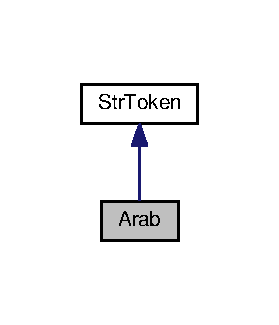
\includegraphics[width=134pt]{class_arab__inherit__graph}
\end{center}
\end{figure}


Collaboration diagram for Arab\-:\nopagebreak
\begin{figure}[H]
\begin{center}
\leavevmode
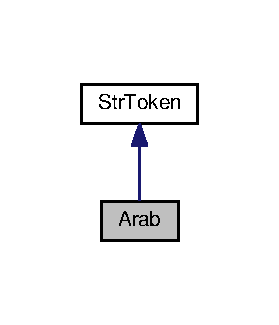
\includegraphics[width=134pt]{class_arab__coll__graph}
\end{center}
\end{figure}
\subsection*{Public Member Functions}
\begin{DoxyCompactItemize}
\item 
virtual bool \hyperlink{class_arab_ab7f0cbcaf9b248b8545b22ccec07a8cd}{can\-Convert} (const std\-::string \&s)
\begin{DoxyCompactList}\small\item\em mengembalikan true bila s dapat dikonversi ke token \end{DoxyCompactList}\item 
virtual std\-::string \hyperlink{class_arab_a097a31788290644f61e76001d7180ec1}{to\-String} (const \hyperlink{class_token}{Token} \&T)
\begin{DoxyCompactList}\small\item\em mengembalikan representasi string dari token T \end{DoxyCompactList}\item 
virtual \hyperlink{class_token}{Token} \hyperlink{class_arab_a107f2bde10c4cd4dfd18a44db5739b4c}{to\-Token} (const std\-::string \&s)
\begin{DoxyCompactList}\small\item\em mengembalikan representasi token dari string s \end{DoxyCompactList}\end{DoxyCompactItemize}


\subsection{Detailed Description}
Responsibility\par
Kelas ini merupakan implementasi kelas \hyperlink{class_str_token}{Str\-Token} dengan konversi sesuai aturan bilangan arab\par
Hubungan dengan kelas lain\par
mengimplementasi \hyperlink{class_str_token}{Str\-Token}\par
Gambaran umum method\par
metodanya adalah implementasi metoda \hyperlink{class_str_token}{Str\-Token}\par


\subsection{Member Function Documentation}
\hypertarget{class_arab_ab7f0cbcaf9b248b8545b22ccec07a8cd}{\index{Arab@{Arab}!can\-Convert@{can\-Convert}}
\index{can\-Convert@{can\-Convert}!Arab@{Arab}}
\subsubsection[{can\-Convert}]{\setlength{\rightskip}{0pt plus 5cm}bool Arab\-::can\-Convert (
\begin{DoxyParamCaption}
\item[{const std\-::string \&}]{s}
\end{DoxyParamCaption}
)\hspace{0.3cm}{\ttfamily [virtual]}}}\label{class_arab_ab7f0cbcaf9b248b8545b22ccec07a8cd}


mengembalikan true bila s dapat dikonversi ke token 



Implements \hyperlink{class_str_token_acd92c843b3b092c21d5a038c5d336957}{Str\-Token}.

\hypertarget{class_arab_a097a31788290644f61e76001d7180ec1}{\index{Arab@{Arab}!to\-String@{to\-String}}
\index{to\-String@{to\-String}!Arab@{Arab}}
\subsubsection[{to\-String}]{\setlength{\rightskip}{0pt plus 5cm}std\-::string Arab\-::to\-String (
\begin{DoxyParamCaption}
\item[{const {\bf Token} \&}]{T}
\end{DoxyParamCaption}
)\hspace{0.3cm}{\ttfamily [virtual]}}}\label{class_arab_a097a31788290644f61e76001d7180ec1}


mengembalikan representasi string dari token T 



Implements \hyperlink{class_str_token_a9562cf6aff9cefa7a223d78573755e8e}{Str\-Token}.

\hypertarget{class_arab_a107f2bde10c4cd4dfd18a44db5739b4c}{\index{Arab@{Arab}!to\-Token@{to\-Token}}
\index{to\-Token@{to\-Token}!Arab@{Arab}}
\subsubsection[{to\-Token}]{\setlength{\rightskip}{0pt plus 5cm}{\bf Token} Arab\-::to\-Token (
\begin{DoxyParamCaption}
\item[{const std\-::string \&}]{s}
\end{DoxyParamCaption}
)\hspace{0.3cm}{\ttfamily [virtual]}}}\label{class_arab_a107f2bde10c4cd4dfd18a44db5739b4c}


mengembalikan representasi token dari string s 



Implements \hyperlink{class_str_token_ae3f06fac8d7030218db0d833fae6f773}{Str\-Token}.



The documentation for this class was generated from the following files\-:\begin{DoxyCompactItemize}
\item 
/home/nim\-\_\-13512501/\-Documents/tubes 1 O\-O\-P/src/token/\hyperlink{_arab_8h}{Arab.\-h}\item 
/home/nim\-\_\-13512501/\-Documents/tubes 1 O\-O\-P/src/token/\hyperlink{_arab_8cpp}{Arab.\-cpp}\end{DoxyCompactItemize}

\hypertarget{class_converter}{\section{Converter Class Reference}
\label{class_converter}\index{Converter@{Converter}}
}


{\ttfamily \#include $<$converter.\-h$>$}

\subsection*{Public Types}
\begin{DoxyCompactItemize}
\item 
enum \hyperlink{class_converter_a1caaefa1f3fba463bd215e8e7f12872f}{Tipe\-Representasi\-Bilangan} \{ \hyperlink{class_converter_a1caaefa1f3fba463bd215e8e7f12872fa42f9bbd983a4ccdf72f2fc2bfe26efe7}{\-\_\-\-Arab}, 
\hyperlink{class_converter_a1caaefa1f3fba463bd215e8e7f12872faab56d50b2561f79548c4fc6e700d7005}{\-\_\-\-Romawi}, 
\hyperlink{class_converter_a1caaefa1f3fba463bd215e8e7f12872fa5688eeb94a505273115a1f2f75d40212}{\-\_\-\-Logika}
 \}
\end{DoxyCompactItemize}
\subsection*{Public Member Functions}
\begin{DoxyCompactItemize}
\item 
std\-::string \hyperlink{class_converter_a8a22c530d91f9b0de64c28cb990dc6bb}{to\-String} (const \hyperlink{class_token}{Token} \&)
\begin{DoxyCompactList}\small\item\em mengkonversi token ke string \end{DoxyCompactList}\item 
\hyperlink{class_token}{Token} \hyperlink{class_converter_aa7b74352c29c5bcf28ed85cf892f3517}{to\-Token} (const std\-::string \&)
\begin{DoxyCompactList}\small\item\em mengkonversi string ke token. melempar exception bila gagal \end{DoxyCompactList}\item 
void \hyperlink{class_converter_a4897e820fd8ab55da965cefda2901fc1}{Set\-Mode} (\hyperlink{class_converter_a1caaefa1f3fba463bd215e8e7f12872f}{Tipe\-Representasi\-Bilangan})
\begin{DoxyCompactList}\small\item\em mengeset apakah converter menggunakan bilangan \-\_\-\-Arab, \-\_\-\-Romawi, atau \-\_\-\-Logika \end{DoxyCompactList}\item 
void \hyperlink{class_converter_a60a0c269a84ec77acf6a7f4ee9ce589e}{Set\-Str\-Operator} (const std\-::string \&, \hyperlink{_token_8h_a29ea73031d51befacf649fa6af865e30}{Tipe\-Token})
\begin{DoxyCompactList}\small\item\em mengeset representasi operator \end{DoxyCompactList}\end{DoxyCompactItemize}
{\bf }\par
\begin{DoxyCompactItemize}
\item 
\hyperlink{class_converter_a1de81f3e06093411e5d27ce882bc010f}{Converter} ()
\item 
\hyperlink{class_converter_a11cf08fca2f84ab67fec9b935badca90}{Converter} (const \hyperlink{class_converter}{Converter} \&C)
\item 
\hyperlink{class_converter_a9ecd05695a52c03158b81e544e13b996}{$\sim$\-Converter} ()
\item 
\hyperlink{class_converter}{Converter} \& \hyperlink{class_converter_addd00b03af5ab50e3586e7889e6d6ce9}{operator=} (const \hyperlink{class_converter}{Converter} \&C)
\end{DoxyCompactItemize}



\subsection{Detailed Description}
Responsibility Kelas ini bertugas mengkonversi seluruh kata yang valid menjadi token, baik operand maupun operator Hubungan dengan kelas lain Ia merupakan agregasi dari \hyperlink{class_str_token}{Str\-Token} dan/atau Turunannya Gambaran umum method metodanya adalah to\-String dan to\-Token. 

\subsection{Member Enumeration Documentation}
\hypertarget{class_converter_a1caaefa1f3fba463bd215e8e7f12872f}{\index{Converter@{Converter}!Tipe\-Representasi\-Bilangan@{Tipe\-Representasi\-Bilangan}}
\index{Tipe\-Representasi\-Bilangan@{Tipe\-Representasi\-Bilangan}!Converter@{Converter}}
\subsubsection[{Tipe\-Representasi\-Bilangan}]{\setlength{\rightskip}{0pt plus 5cm}enum {\bf Converter\-::\-Tipe\-Representasi\-Bilangan}}}\label{class_converter_a1caaefa1f3fba463bd215e8e7f12872f}
\begin{Desc}
\item[Enumerator]\par
\begin{description}
\index{\-\_\-\-Arab@{\-\_\-\-Arab}!Converter@{Converter}}\index{Converter@{Converter}!\-\_\-\-Arab@{\-\_\-\-Arab}}\item[{\em 
\hypertarget{class_converter_a1caaefa1f3fba463bd215e8e7f12872fa42f9bbd983a4ccdf72f2fc2bfe26efe7}{\-\_\-\-Arab}\label{class_converter_a1caaefa1f3fba463bd215e8e7f12872fa42f9bbd983a4ccdf72f2fc2bfe26efe7}
}]\index{\-\_\-\-Romawi@{\-\_\-\-Romawi}!Converter@{Converter}}\index{Converter@{Converter}!\-\_\-\-Romawi@{\-\_\-\-Romawi}}\item[{\em 
\hypertarget{class_converter_a1caaefa1f3fba463bd215e8e7f12872faab56d50b2561f79548c4fc6e700d7005}{\-\_\-\-Romawi}\label{class_converter_a1caaefa1f3fba463bd215e8e7f12872faab56d50b2561f79548c4fc6e700d7005}
}]\index{\-\_\-\-Logika@{\-\_\-\-Logika}!Converter@{Converter}}\index{Converter@{Converter}!\-\_\-\-Logika@{\-\_\-\-Logika}}\item[{\em 
\hypertarget{class_converter_a1caaefa1f3fba463bd215e8e7f12872fa5688eeb94a505273115a1f2f75d40212}{\-\_\-\-Logika}\label{class_converter_a1caaefa1f3fba463bd215e8e7f12872fa5688eeb94a505273115a1f2f75d40212}
}]\end{description}
\end{Desc}


\subsection{Constructor \& Destructor Documentation}
\hypertarget{class_converter_a1de81f3e06093411e5d27ce882bc010f}{\index{Converter@{Converter}!Converter@{Converter}}
\index{Converter@{Converter}!Converter@{Converter}}
\subsubsection[{Converter}]{\setlength{\rightskip}{0pt plus 5cm}Converter\-::\-Converter (
\begin{DoxyParamCaption}
{}
\end{DoxyParamCaption}
)}}\label{class_converter_a1de81f3e06093411e5d27ce882bc010f}
cctor,ctor,dtor

default\-: operator default dan bilangan arab \hypertarget{class_converter_a11cf08fca2f84ab67fec9b935badca90}{\index{Converter@{Converter}!Converter@{Converter}}
\index{Converter@{Converter}!Converter@{Converter}}
\subsubsection[{Converter}]{\setlength{\rightskip}{0pt plus 5cm}Converter\-::\-Converter (
\begin{DoxyParamCaption}
\item[{const {\bf Converter} \&}]{C}
\end{DoxyParamCaption}
)}}\label{class_converter_a11cf08fca2f84ab67fec9b935badca90}
\hypertarget{class_converter_a9ecd05695a52c03158b81e544e13b996}{\index{Converter@{Converter}!$\sim$\-Converter@{$\sim$\-Converter}}
\index{$\sim$\-Converter@{$\sim$\-Converter}!Converter@{Converter}}
\subsubsection[{$\sim$\-Converter}]{\setlength{\rightskip}{0pt plus 5cm}Converter\-::$\sim$\-Converter (
\begin{DoxyParamCaption}
{}
\end{DoxyParamCaption}
)}}\label{class_converter_a9ecd05695a52c03158b81e544e13b996}


\subsection{Member Function Documentation}
\hypertarget{class_converter_addd00b03af5ab50e3586e7889e6d6ce9}{\index{Converter@{Converter}!operator=@{operator=}}
\index{operator=@{operator=}!Converter@{Converter}}
\subsubsection[{operator=}]{\setlength{\rightskip}{0pt plus 5cm}{\bf Converter} \& Converter\-::operator= (
\begin{DoxyParamCaption}
\item[{const {\bf Converter} \&}]{C}
\end{DoxyParamCaption}
)}}\label{class_converter_addd00b03af5ab50e3586e7889e6d6ce9}
\hypertarget{class_converter_a4897e820fd8ab55da965cefda2901fc1}{\index{Converter@{Converter}!Set\-Mode@{Set\-Mode}}
\index{Set\-Mode@{Set\-Mode}!Converter@{Converter}}
\subsubsection[{Set\-Mode}]{\setlength{\rightskip}{0pt plus 5cm}void Converter\-::\-Set\-Mode (
\begin{DoxyParamCaption}
\item[{{\bf Tipe\-Representasi\-Bilangan}}]{T\-R\-B}
\end{DoxyParamCaption}
)}}\label{class_converter_a4897e820fd8ab55da965cefda2901fc1}


mengeset apakah converter menggunakan bilangan \-\_\-\-Arab, \-\_\-\-Romawi, atau \-\_\-\-Logika 

\hypertarget{class_converter_a60a0c269a84ec77acf6a7f4ee9ce589e}{\index{Converter@{Converter}!Set\-Str\-Operator@{Set\-Str\-Operator}}
\index{Set\-Str\-Operator@{Set\-Str\-Operator}!Converter@{Converter}}
\subsubsection[{Set\-Str\-Operator}]{\setlength{\rightskip}{0pt plus 5cm}void Converter\-::\-Set\-Str\-Operator (
\begin{DoxyParamCaption}
\item[{const std\-::string \&}]{s, }
\item[{{\bf Tipe\-Token}}]{tt}
\end{DoxyParamCaption}
)}}\label{class_converter_a60a0c269a84ec77acf6a7f4ee9ce589e}


mengeset representasi operator 

\hypertarget{class_converter_a8a22c530d91f9b0de64c28cb990dc6bb}{\index{Converter@{Converter}!to\-String@{to\-String}}
\index{to\-String@{to\-String}!Converter@{Converter}}
\subsubsection[{to\-String}]{\setlength{\rightskip}{0pt plus 5cm}std\-::string Converter\-::to\-String (
\begin{DoxyParamCaption}
\item[{const {\bf Token} \&}]{T}
\end{DoxyParamCaption}
)}}\label{class_converter_a8a22c530d91f9b0de64c28cb990dc6bb}


mengkonversi token ke string 

\hypertarget{class_converter_aa7b74352c29c5bcf28ed85cf892f3517}{\index{Converter@{Converter}!to\-Token@{to\-Token}}
\index{to\-Token@{to\-Token}!Converter@{Converter}}
\subsubsection[{to\-Token}]{\setlength{\rightskip}{0pt plus 5cm}{\bf Token} Converter\-::to\-Token (
\begin{DoxyParamCaption}
\item[{const std\-::string \&}]{s}
\end{DoxyParamCaption}
)}}\label{class_converter_aa7b74352c29c5bcf28ed85cf892f3517}


mengkonversi string ke token. melempar exception bila gagal 



The documentation for this class was generated from the following files\-:\begin{DoxyCompactItemize}
\item 
/home/nim\-\_\-13512501/\-Documents/tubes 1 O\-O\-P/src/token/\hyperlink{converter_8h}{converter.\-h}\item 
/home/nim\-\_\-13512501/\-Documents/tubes 1 O\-O\-P/src/token/\hyperlink{converter_8cpp}{converter.\-cpp}\end{DoxyCompactItemize}

\hypertarget{class_converter_exception}{\section{Converter\-Exception Class Reference}
\label{class_converter_exception}\index{Converter\-Exception@{Converter\-Exception}}
}


{\ttfamily \#include $<$converter.\-h$>$}



Inheritance diagram for Converter\-Exception\-:\nopagebreak
\begin{figure}[H]
\begin{center}
\leavevmode
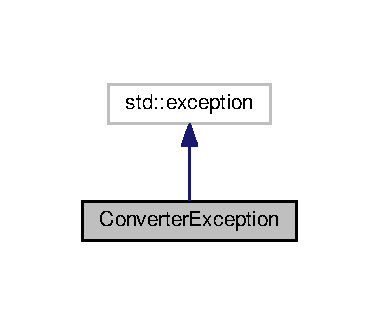
\includegraphics[width=182pt]{class_converter_exception__inherit__graph}
\end{center}
\end{figure}


Collaboration diagram for Converter\-Exception\-:\nopagebreak
\begin{figure}[H]
\begin{center}
\leavevmode
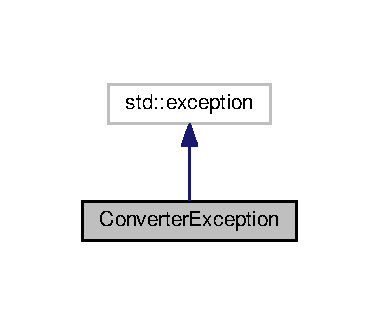
\includegraphics[width=182pt]{class_converter_exception__coll__graph}
\end{center}
\end{figure}
\subsection*{Public Member Functions}
\begin{DoxyCompactItemize}
\item 
\hyperlink{class_converter_exception_ae452451034ab567d0d9e3c876b528017}{Converter\-Exception} ()
\item 
\hyperlink{class_converter_exception_aedf2569f75ffeb9334a0a9e100c2e765}{Converter\-Exception} (const char $\ast$\-\_\-msg)
\item 
virtual const char $\ast$ \hyperlink{class_converter_exception_a8cc1a60f8224cff62ac68d58fec565f3}{what} () const   throw ()
\end{DoxyCompactItemize}
\subsection*{Static Public Attributes}
\begin{DoxyCompactItemize}
\item 
static const int \hyperlink{class_converter_exception_aa85a77630be23abdc85b783083ac7380}{msg\-\_\-maxlength}
\end{DoxyCompactItemize}


\subsection{Detailed Description}
kelas exception yang dilempar kelas converter 

\subsection{Constructor \& Destructor Documentation}
\hypertarget{class_converter_exception_ae452451034ab567d0d9e3c876b528017}{\index{Converter\-Exception@{Converter\-Exception}!Converter\-Exception@{Converter\-Exception}}
\index{Converter\-Exception@{Converter\-Exception}!ConverterException@{Converter\-Exception}}
\subsubsection[{Converter\-Exception}]{\setlength{\rightskip}{0pt plus 5cm}Converter\-Exception\-::\-Converter\-Exception (
\begin{DoxyParamCaption}
{}
\end{DoxyParamCaption}
)\hspace{0.3cm}{\ttfamily [inline]}}}\label{class_converter_exception_ae452451034ab567d0d9e3c876b528017}
\hypertarget{class_converter_exception_aedf2569f75ffeb9334a0a9e100c2e765}{\index{Converter\-Exception@{Converter\-Exception}!Converter\-Exception@{Converter\-Exception}}
\index{Converter\-Exception@{Converter\-Exception}!ConverterException@{Converter\-Exception}}
\subsubsection[{Converter\-Exception}]{\setlength{\rightskip}{0pt plus 5cm}Converter\-Exception\-::\-Converter\-Exception (
\begin{DoxyParamCaption}
\item[{const char $\ast$}]{\-\_\-msg}
\end{DoxyParamCaption}
)\hspace{0.3cm}{\ttfamily [inline]}}}\label{class_converter_exception_aedf2569f75ffeb9334a0a9e100c2e765}


\subsection{Member Function Documentation}
\hypertarget{class_converter_exception_a8cc1a60f8224cff62ac68d58fec565f3}{\index{Converter\-Exception@{Converter\-Exception}!what@{what}}
\index{what@{what}!ConverterException@{Converter\-Exception}}
\subsubsection[{what}]{\setlength{\rightskip}{0pt plus 5cm}virtual const char$\ast$ Converter\-Exception\-::what (
\begin{DoxyParamCaption}
{}
\end{DoxyParamCaption}
) const throw  ) \hspace{0.3cm}{\ttfamily [inline]}, {\ttfamily [virtual]}}}\label{class_converter_exception_a8cc1a60f8224cff62ac68d58fec565f3}


\subsection{Member Data Documentation}
\hypertarget{class_converter_exception_aa85a77630be23abdc85b783083ac7380}{\index{Converter\-Exception@{Converter\-Exception}!msg\-\_\-maxlength@{msg\-\_\-maxlength}}
\index{msg\-\_\-maxlength@{msg\-\_\-maxlength}!ConverterException@{Converter\-Exception}}
\subsubsection[{msg\-\_\-maxlength}]{\setlength{\rightskip}{0pt plus 5cm}const int Converter\-Exception\-::msg\-\_\-maxlength\hspace{0.3cm}{\ttfamily [static]}}}\label{class_converter_exception_aa85a77630be23abdc85b783083ac7380}


The documentation for this class was generated from the following file\-:\begin{DoxyCompactItemize}
\item 
/home/nim\-\_\-13512501/\-Documents/tubes 1 O\-O\-P/src/token/\hyperlink{converter_8h}{converter.\-h}\end{DoxyCompactItemize}

\hypertarget{class_evaluator}{\section{Evaluator Class Reference}
\label{class_evaluator}\index{Evaluator@{Evaluator}}
}


{\ttfamily \#include $<$Evaluator.\-h$>$}

\subsection*{Public Member Functions}
\begin{DoxyCompactItemize}
\item 
\hyperlink{class_evaluator_ab0fae467aa1c3870f9cfb0c8368710be}{Evaluator} ()
\item 
string \hyperlink{class_evaluator_a2b676b6f20467704c56df20b31cff5b3}{Do\-Cmd} (string, bool add\-To\-History=true)
\begin{DoxyCompactList}\small\item\em melakukan perintah \end{DoxyCompactList}\item 
string \hyperlink{class_evaluator_afcc41151e1e6ad0d07bbb4224dd74629}{Redo} (int)
\begin{DoxyCompactList}\small\item\em mengulang n buah perintah \end{DoxyCompactList}\item 
string \hyperlink{class_evaluator_ab2c3addba566d6259b99def095bbbc5d}{Mem\-All} ()
\begin{DoxyCompactList}\small\item\em menampilkan semua perintah \end{DoxyCompactList}\item 
string \hyperlink{class_evaluator_a4ceb00f94149585a46cc35ef41928899}{Mem} (int)
\begin{DoxyCompactList}\small\item\em menampilkan n buah perintah \end{DoxyCompactList}\item 
string \hyperlink{class_evaluator_ad82d60da69a7c7a1189778e0032c4a73}{Undo} (int)
\begin{DoxyCompactList}\small\item\em menghapus n buah perintah \end{DoxyCompactList}\item 
string \hyperlink{class_evaluator_aeb82037e6e511050a4e7511b765e990a}{Compute\-Expr} (string)
\begin{DoxyCompactList}\small\item\em menghitung ekspresi, menggunakan mesin token dan stack \end{DoxyCompactList}\item 
string \hyperlink{class_evaluator_aa62da9339a78c89f246dbe827951515a}{Compute\-Expr\-Prefix} (string)
\begin{DoxyCompactList}\small\item\em menghitung ekspresi prefix \end{DoxyCompactList}\item 
string \hyperlink{class_evaluator_a7672b370d77902ad183223846820b212}{Compute\-Expr\-Infix} (string)
\begin{DoxyCompactList}\small\item\em menghitung ekspresi infix \end{DoxyCompactList}\item 
string \hyperlink{class_evaluator_a72f837e9d38d47d599a43f3c4e60aef5}{Compute\-Expr\-Postfix} (string)
\begin{DoxyCompactList}\small\item\em menghitung ekspresi postfix \end{DoxyCompactList}\item 
string \hyperlink{class_evaluator_a3fe98d459400fd7a458456cd6f5e2d91}{Save} ()
\begin{DoxyCompactList}\small\item\em menyimpan histori \end{DoxyCompactList}\item 
string \hyperlink{class_evaluator_a09afbb85d94fe5dd7107676b1ec6bc4b}{Set} (string s)
\begin{DoxyCompactList}\small\item\em melakukan setting \end{DoxyCompactList}\item 
void \hyperlink{class_evaluator_aef032056072f0d51c7e126857653de5b}{Quit} ()
\begin{DoxyCompactList}\small\item\em keluar \end{DoxyCompactList}\end{DoxyCompactItemize}


\subsection{Constructor \& Destructor Documentation}
\hypertarget{class_evaluator_ab0fae467aa1c3870f9cfb0c8368710be}{\index{Evaluator@{Evaluator}!Evaluator@{Evaluator}}
\index{Evaluator@{Evaluator}!Evaluator@{Evaluator}}
\subsubsection[{Evaluator}]{\setlength{\rightskip}{0pt plus 5cm}Evaluator\-::\-Evaluator (
\begin{DoxyParamCaption}
{}
\end{DoxyParamCaption}
)\hspace{0.3cm}{\ttfamily [inline]}}}\label{class_evaluator_ab0fae467aa1c3870f9cfb0c8368710be}
ctor default\-: 

\subsection{Member Function Documentation}
\hypertarget{class_evaluator_aeb82037e6e511050a4e7511b765e990a}{\index{Evaluator@{Evaluator}!Compute\-Expr@{Compute\-Expr}}
\index{Compute\-Expr@{Compute\-Expr}!Evaluator@{Evaluator}}
\subsubsection[{Compute\-Expr}]{\setlength{\rightskip}{0pt plus 5cm}string Evaluator\-::\-Compute\-Expr (
\begin{DoxyParamCaption}
\item[{string}]{s}
\end{DoxyParamCaption}
)}}\label{class_evaluator_aeb82037e6e511050a4e7511b765e990a}


menghitung ekspresi, menggunakan mesin token dan stack 

\hypertarget{class_evaluator_a7672b370d77902ad183223846820b212}{\index{Evaluator@{Evaluator}!Compute\-Expr\-Infix@{Compute\-Expr\-Infix}}
\index{Compute\-Expr\-Infix@{Compute\-Expr\-Infix}!Evaluator@{Evaluator}}
\subsubsection[{Compute\-Expr\-Infix}]{\setlength{\rightskip}{0pt plus 5cm}string Evaluator\-::\-Compute\-Expr\-Infix (
\begin{DoxyParamCaption}
\item[{string}]{s}
\end{DoxyParamCaption}
)}}\label{class_evaluator_a7672b370d77902ad183223846820b212}


menghitung ekspresi infix 

\hypertarget{class_evaluator_a72f837e9d38d47d599a43f3c4e60aef5}{\index{Evaluator@{Evaluator}!Compute\-Expr\-Postfix@{Compute\-Expr\-Postfix}}
\index{Compute\-Expr\-Postfix@{Compute\-Expr\-Postfix}!Evaluator@{Evaluator}}
\subsubsection[{Compute\-Expr\-Postfix}]{\setlength{\rightskip}{0pt plus 5cm}string Evaluator\-::\-Compute\-Expr\-Postfix (
\begin{DoxyParamCaption}
\item[{string}]{s}
\end{DoxyParamCaption}
)}}\label{class_evaluator_a72f837e9d38d47d599a43f3c4e60aef5}


menghitung ekspresi postfix 

\hypertarget{class_evaluator_aa62da9339a78c89f246dbe827951515a}{\index{Evaluator@{Evaluator}!Compute\-Expr\-Prefix@{Compute\-Expr\-Prefix}}
\index{Compute\-Expr\-Prefix@{Compute\-Expr\-Prefix}!Evaluator@{Evaluator}}
\subsubsection[{Compute\-Expr\-Prefix}]{\setlength{\rightskip}{0pt plus 5cm}string Evaluator\-::\-Compute\-Expr\-Prefix (
\begin{DoxyParamCaption}
\item[{string}]{s}
\end{DoxyParamCaption}
)}}\label{class_evaluator_aa62da9339a78c89f246dbe827951515a}


menghitung ekspresi prefix 

\hypertarget{class_evaluator_a2b676b6f20467704c56df20b31cff5b3}{\index{Evaluator@{Evaluator}!Do\-Cmd@{Do\-Cmd}}
\index{Do\-Cmd@{Do\-Cmd}!Evaluator@{Evaluator}}
\subsubsection[{Do\-Cmd}]{\setlength{\rightskip}{0pt plus 5cm}string Evaluator\-::\-Do\-Cmd (
\begin{DoxyParamCaption}
\item[{string}]{s, }
\item[{bool}]{add\-To\-History = {\ttfamily true}}
\end{DoxyParamCaption}
)}}\label{class_evaluator_a2b676b6f20467704c56df20b31cff5b3}


melakukan perintah 

\hypertarget{class_evaluator_a4ceb00f94149585a46cc35ef41928899}{\index{Evaluator@{Evaluator}!Mem@{Mem}}
\index{Mem@{Mem}!Evaluator@{Evaluator}}
\subsubsection[{Mem}]{\setlength{\rightskip}{0pt plus 5cm}string Evaluator\-::\-Mem (
\begin{DoxyParamCaption}
\item[{int}]{n}
\end{DoxyParamCaption}
)}}\label{class_evaluator_a4ceb00f94149585a46cc35ef41928899}


menampilkan n buah perintah 

\hypertarget{class_evaluator_ab2c3addba566d6259b99def095bbbc5d}{\index{Evaluator@{Evaluator}!Mem\-All@{Mem\-All}}
\index{Mem\-All@{Mem\-All}!Evaluator@{Evaluator}}
\subsubsection[{Mem\-All}]{\setlength{\rightskip}{0pt plus 5cm}string Evaluator\-::\-Mem\-All (
\begin{DoxyParamCaption}
{}
\end{DoxyParamCaption}
)}}\label{class_evaluator_ab2c3addba566d6259b99def095bbbc5d}


menampilkan semua perintah 

\hypertarget{class_evaluator_aef032056072f0d51c7e126857653de5b}{\index{Evaluator@{Evaluator}!Quit@{Quit}}
\index{Quit@{Quit}!Evaluator@{Evaluator}}
\subsubsection[{Quit}]{\setlength{\rightskip}{0pt plus 5cm}void Evaluator\-::\-Quit (
\begin{DoxyParamCaption}
{}
\end{DoxyParamCaption}
)}}\label{class_evaluator_aef032056072f0d51c7e126857653de5b}


keluar 

\hypertarget{class_evaluator_afcc41151e1e6ad0d07bbb4224dd74629}{\index{Evaluator@{Evaluator}!Redo@{Redo}}
\index{Redo@{Redo}!Evaluator@{Evaluator}}
\subsubsection[{Redo}]{\setlength{\rightskip}{0pt plus 5cm}string Evaluator\-::\-Redo (
\begin{DoxyParamCaption}
\item[{int}]{n}
\end{DoxyParamCaption}
)}}\label{class_evaluator_afcc41151e1e6ad0d07bbb4224dd74629}


mengulang n buah perintah 

\hypertarget{class_evaluator_a3fe98d459400fd7a458456cd6f5e2d91}{\index{Evaluator@{Evaluator}!Save@{Save}}
\index{Save@{Save}!Evaluator@{Evaluator}}
\subsubsection[{Save}]{\setlength{\rightskip}{0pt plus 5cm}string Evaluator\-::\-Save (
\begin{DoxyParamCaption}
{}
\end{DoxyParamCaption}
)}}\label{class_evaluator_a3fe98d459400fd7a458456cd6f5e2d91}


menyimpan histori 

\hypertarget{class_evaluator_a09afbb85d94fe5dd7107676b1ec6bc4b}{\index{Evaluator@{Evaluator}!Set@{Set}}
\index{Set@{Set}!Evaluator@{Evaluator}}
\subsubsection[{Set}]{\setlength{\rightskip}{0pt plus 5cm}string Evaluator\-::\-Set (
\begin{DoxyParamCaption}
\item[{string}]{s}
\end{DoxyParamCaption}
)}}\label{class_evaluator_a09afbb85d94fe5dd7107676b1ec6bc4b}


melakukan setting 

sebuah finite state machine untuk mengubah pengaturan \hypertarget{class_evaluator_ad82d60da69a7c7a1189778e0032c4a73}{\index{Evaluator@{Evaluator}!Undo@{Undo}}
\index{Undo@{Undo}!Evaluator@{Evaluator}}
\subsubsection[{Undo}]{\setlength{\rightskip}{0pt plus 5cm}string Evaluator\-::\-Undo (
\begin{DoxyParamCaption}
\item[{int}]{n}
\end{DoxyParamCaption}
)}}\label{class_evaluator_ad82d60da69a7c7a1189778e0032c4a73}


menghapus n buah perintah 



The documentation for this class was generated from the following files\-:\begin{DoxyCompactItemize}
\item 
/home/nim\-\_\-13512501/\-Documents/tubes 1 O\-O\-P/src/\hyperlink{_evaluator_8h}{Evaluator.\-h}\item 
/home/nim\-\_\-13512501/\-Documents/tubes 1 O\-O\-P/src/\hyperlink{_evaluator_8cpp}{Evaluator.\-cpp}\end{DoxyCompactItemize}

\hypertarget{class_file_manager}{\section{File\-Manager Class Reference}
\label{class_file_manager}\index{File\-Manager@{File\-Manager}}
}


{\ttfamily \#include $<$File\-Manager.\-h$>$}

\subsection*{Public Member Functions}
\begin{DoxyCompactItemize}
\item 
void \hyperlink{class_file_manager_a32b54e894a1ec6af3a33a00c6c6b3d29}{Save} (\hyperlink{class_history}{History} H)
\begin{DoxyCompactList}\small\item\em menyimpan ke berkas dengan tambahan informasi tanggal dan jam \end{DoxyCompactList}\end{DoxyCompactItemize}


\subsection{Detailed Description}
Responsibility\par
kelas ini bertugas menyimpan histori ke berkas\par
Hubungan dengan kelas lain\par
kelas ini menggunakan kelas Histori pada salah satu metodanya\par
Gambaran umum method\par
kelas ini memiliki metoda Save\par


\subsection{Member Function Documentation}
\hypertarget{class_file_manager_a32b54e894a1ec6af3a33a00c6c6b3d29}{\index{File\-Manager@{File\-Manager}!Save@{Save}}
\index{Save@{Save}!FileManager@{File\-Manager}}
\subsubsection[{Save}]{\setlength{\rightskip}{0pt plus 5cm}void File\-Manager\-::\-Save (
\begin{DoxyParamCaption}
\item[{{\bf History}}]{H}
\end{DoxyParamCaption}
)}}\label{class_file_manager_a32b54e894a1ec6af3a33a00c6c6b3d29}


menyimpan ke berkas dengan tambahan informasi tanggal dan jam 



The documentation for this class was generated from the following files\-:\begin{DoxyCompactItemize}
\item 
/home/nim\-\_\-13512501/\-Documents/tubes 1 O\-O\-P/src/\hyperlink{_file_manager_8h}{File\-Manager.\-h}\item 
/home/nim\-\_\-13512501/\-Documents/tubes 1 O\-O\-P/src/\hyperlink{_file_manager_8cpp}{File\-Manager.\-cpp}\end{DoxyCompactItemize}

\hypertarget{class_file_manager_exception}{\section{File\-Manager\-Exception Class Reference}
\label{class_file_manager_exception}\index{File\-Manager\-Exception@{File\-Manager\-Exception}}
}


exception yang dilempar oleh \hyperlink{class_file_manager}{File\-Manager}  




{\ttfamily \#include $<$File\-Manager.\-h$>$}



Inheritance diagram for File\-Manager\-Exception\-:\nopagebreak
\begin{figure}[H]
\begin{center}
\leavevmode
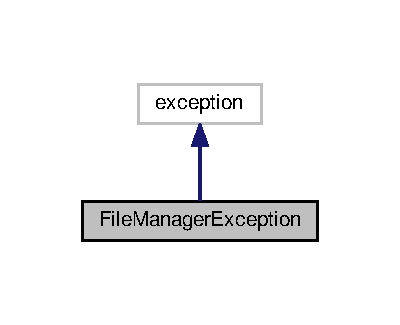
\includegraphics[width=192pt]{class_file_manager_exception__inherit__graph}
\end{center}
\end{figure}


Collaboration diagram for File\-Manager\-Exception\-:\nopagebreak
\begin{figure}[H]
\begin{center}
\leavevmode
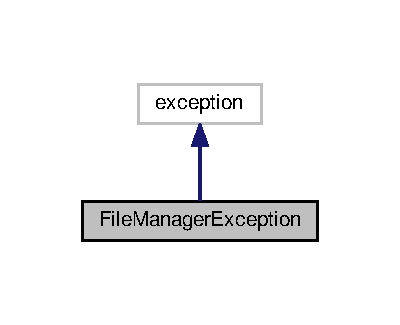
\includegraphics[width=192pt]{class_file_manager_exception__coll__graph}
\end{center}
\end{figure}
\subsection*{Public Member Functions}
\begin{DoxyCompactItemize}
\item 
virtual const char $\ast$ \hyperlink{class_file_manager_exception_a4d2ded04871dadef8fae6978517fa6e2}{what} () const   throw ()
\end{DoxyCompactItemize}


\subsection{Detailed Description}
exception yang dilempar oleh \hyperlink{class_file_manager}{File\-Manager} 

\subsection{Member Function Documentation}
\hypertarget{class_file_manager_exception_a4d2ded04871dadef8fae6978517fa6e2}{\index{File\-Manager\-Exception@{File\-Manager\-Exception}!what@{what}}
\index{what@{what}!FileManagerException@{File\-Manager\-Exception}}
\subsubsection[{what}]{\setlength{\rightskip}{0pt plus 5cm}virtual const char$\ast$ File\-Manager\-Exception\-::what (
\begin{DoxyParamCaption}
{}
\end{DoxyParamCaption}
) const throw  ) \hspace{0.3cm}{\ttfamily [inline]}, {\ttfamily [virtual]}}}\label{class_file_manager_exception_a4d2ded04871dadef8fae6978517fa6e2}


The documentation for this class was generated from the following file\-:\begin{DoxyCompactItemize}
\item 
/home/nim\-\_\-13512501/\-Documents/tubes 1 O\-O\-P/src/\hyperlink{_file_manager_8h}{File\-Manager.\-h}\end{DoxyCompactItemize}

\hypertarget{class_history}{\section{History Class Reference}
\label{class_history}\index{History@{History}}
}


{\ttfamily \#include $<$history.\-h$>$}

\subsection*{Public Member Functions}
\begin{DoxyCompactItemize}
\item 
\hyperlink{class_history_afba1384643f419d079e78adb1497f741}{History} ()
\begin{DoxyCompactList}\small\item\em ctor \end{DoxyCompactList}\item 
\hyperlink{class_history_af05bd873be46b17f9c95e51241aa90b6}{History} (string s, string r)
\item 
\hyperlink{class_history_a1bcdcf0c6384ac7c3ecff90078aa3176}{History} (const \hyperlink{class_history}{History} \&H)
\begin{DoxyCompactList}\small\item\em cctor \end{DoxyCompactList}\item 
\hyperlink{class_history_a5b00b64a1ddee04e60d5a3b517fd6d4c}{$\sim$\-History} ()
\begin{DoxyCompactList}\small\item\em dtor \end{DoxyCompactList}\item 
string \hyperlink{class_history_ac5080f105417eafd73205340db2c9559}{Get\-All\-Both} ()
\begin{DoxyCompactList}\small\item\em predikat \end{DoxyCompactList}\item 
string \hyperlink{class_history_aaca3ead3b1339bbac0d0c2db3d326ef1}{Get\-All\-Cmd} ()
\begin{DoxyCompactList}\small\item\em mengeluarkan seluruh history \end{DoxyCompactList}\item 
string \hyperlink{class_history_a9180b02255bf0e5aa08613a9c0aa2c02}{Get\-Both} (int n)
\begin{DoxyCompactList}\small\item\em mengeluarkan perintah yang pernah dieksekusi \end{DoxyCompactList}\item 
string \hyperlink{class_history_aed23a7f23c25cc960b90f73e678bdd85}{Get\-Cmd} (int n)
\begin{DoxyCompactList}\small\item\em mengeluarkan n buah history terakhir \end{DoxyCompactList}\item 
void \hyperlink{class_history_ae031575124e4d464973c563ab642954d}{Add} (string cmd, string res=\char`\"{}\char`\"{})
\item 
void \hyperlink{class_history_a6b9c6e312f05fb1a076af99117ff73ca}{Delete} (int n)
\end{DoxyCompactItemize}


\subsection{Constructor \& Destructor Documentation}
\hypertarget{class_history_afba1384643f419d079e78adb1497f741}{\index{History@{History}!History@{History}}
\index{History@{History}!History@{History}}
\subsubsection[{History}]{\setlength{\rightskip}{0pt plus 5cm}History\-::\-History (
\begin{DoxyParamCaption}
{}
\end{DoxyParamCaption}
)}}\label{class_history_afba1384643f419d079e78adb1497f741}


ctor 

\hypertarget{class_history_af05bd873be46b17f9c95e51241aa90b6}{\index{History@{History}!History@{History}}
\index{History@{History}!History@{History}}
\subsubsection[{History}]{\setlength{\rightskip}{0pt plus 5cm}History\-::\-History (
\begin{DoxyParamCaption}
\item[{string}]{s, }
\item[{string}]{r}
\end{DoxyParamCaption}
)}}\label{class_history_af05bd873be46b17f9c95e51241aa90b6}
\hypertarget{class_history_a1bcdcf0c6384ac7c3ecff90078aa3176}{\index{History@{History}!History@{History}}
\index{History@{History}!History@{History}}
\subsubsection[{History}]{\setlength{\rightskip}{0pt plus 5cm}History\-::\-History (
\begin{DoxyParamCaption}
\item[{const {\bf History} \&}]{H}
\end{DoxyParamCaption}
)}}\label{class_history_a1bcdcf0c6384ac7c3ecff90078aa3176}


cctor 

\hypertarget{class_history_a5b00b64a1ddee04e60d5a3b517fd6d4c}{\index{History@{History}!$\sim$\-History@{$\sim$\-History}}
\index{$\sim$\-History@{$\sim$\-History}!History@{History}}
\subsubsection[{$\sim$\-History}]{\setlength{\rightskip}{0pt plus 5cm}History\-::$\sim$\-History (
\begin{DoxyParamCaption}
{}
\end{DoxyParamCaption}
)}}\label{class_history_a5b00b64a1ddee04e60d5a3b517fd6d4c}


dtor 



\subsection{Member Function Documentation}
\hypertarget{class_history_ae031575124e4d464973c563ab642954d}{\index{History@{History}!Add@{Add}}
\index{Add@{Add}!History@{History}}
\subsubsection[{Add}]{\setlength{\rightskip}{0pt plus 5cm}void History\-::\-Add (
\begin{DoxyParamCaption}
\item[{string}]{cmd, }
\item[{string}]{res = {\ttfamily \char`\"{}\char`\"{}}}
\end{DoxyParamCaption}
)}}\label{class_history_ae031575124e4d464973c563ab642954d}
\hypertarget{class_history_a6b9c6e312f05fb1a076af99117ff73ca}{\index{History@{History}!Delete@{Delete}}
\index{Delete@{Delete}!History@{History}}
\subsubsection[{Delete}]{\setlength{\rightskip}{0pt plus 5cm}void History\-::\-Delete (
\begin{DoxyParamCaption}
\item[{int}]{n}
\end{DoxyParamCaption}
)}}\label{class_history_a6b9c6e312f05fb1a076af99117ff73ca}
menambahkan perintah cmd dan hasil res I.\-S \hyperlink{class_history}{History} sudah terdefinisi F.\-S cmd dan res sudah ditambah ke dalam history \hypertarget{class_history_ac5080f105417eafd73205340db2c9559}{\index{History@{History}!Get\-All\-Both@{Get\-All\-Both}}
\index{Get\-All\-Both@{Get\-All\-Both}!History@{History}}
\subsubsection[{Get\-All\-Both}]{\setlength{\rightskip}{0pt plus 5cm}string History\-::\-Get\-All\-Both (
\begin{DoxyParamCaption}
{}
\end{DoxyParamCaption}
)}}\label{class_history_ac5080f105417eafd73205340db2c9559}


predikat 

mengeluarkan seluruh history \hypertarget{class_history_aaca3ead3b1339bbac0d0c2db3d326ef1}{\index{History@{History}!Get\-All\-Cmd@{Get\-All\-Cmd}}
\index{Get\-All\-Cmd@{Get\-All\-Cmd}!History@{History}}
\subsubsection[{Get\-All\-Cmd}]{\setlength{\rightskip}{0pt plus 5cm}string History\-::\-Get\-All\-Cmd (
\begin{DoxyParamCaption}
{}
\end{DoxyParamCaption}
)}}\label{class_history_aaca3ead3b1339bbac0d0c2db3d326ef1}


mengeluarkan seluruh history 

mengeluarkan perintah yang pernah dieksekusi \hypertarget{class_history_a9180b02255bf0e5aa08613a9c0aa2c02}{\index{History@{History}!Get\-Both@{Get\-Both}}
\index{Get\-Both@{Get\-Both}!History@{History}}
\subsubsection[{Get\-Both}]{\setlength{\rightskip}{0pt plus 5cm}string History\-::\-Get\-Both (
\begin{DoxyParamCaption}
\item[{int}]{n}
\end{DoxyParamCaption}
)}}\label{class_history_a9180b02255bf0e5aa08613a9c0aa2c02}


mengeluarkan perintah yang pernah dieksekusi 

mengeluarkan n buah history terakhir \hypertarget{class_history_aed23a7f23c25cc960b90f73e678bdd85}{\index{History@{History}!Get\-Cmd@{Get\-Cmd}}
\index{Get\-Cmd@{Get\-Cmd}!History@{History}}
\subsubsection[{Get\-Cmd}]{\setlength{\rightskip}{0pt plus 5cm}string History\-::\-Get\-Cmd (
\begin{DoxyParamCaption}
\item[{int}]{n}
\end{DoxyParamCaption}
)}}\label{class_history_aed23a7f23c25cc960b90f73e678bdd85}


mengeluarkan n buah history terakhir 

mengeluarkan n buah perintah terakhir 

The documentation for this class was generated from the following files\-:\begin{DoxyCompactItemize}
\item 
/home/nim\-\_\-13512501/\-Documents/tubes 1 O\-O\-P/src/\hyperlink{history_8h}{history.\-h}\item 
/home/nim\-\_\-13512501/\-Documents/tubes 1 O\-O\-P/src/\hyperlink{history_8cpp}{history.\-cpp}\end{DoxyCompactItemize}

\hypertarget{class_logika}{\section{Logika Class Reference}
\label{class_logika}\index{Logika@{Logika}}
}


{\ttfamily \#include $<$Logika.\-h$>$}



Inheritance diagram for Logika\-:\nopagebreak
\begin{figure}[H]
\begin{center}
\leavevmode
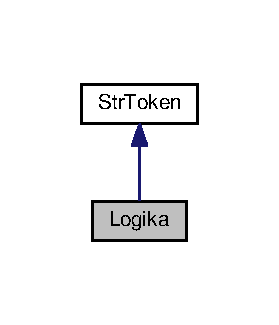
\includegraphics[width=134pt]{class_logika__inherit__graph}
\end{center}
\end{figure}


Collaboration diagram for Logika\-:\nopagebreak
\begin{figure}[H]
\begin{center}
\leavevmode
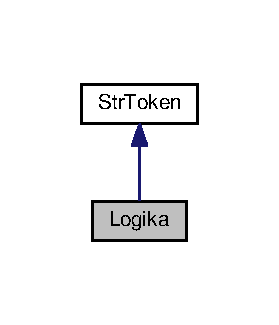
\includegraphics[width=134pt]{class_logika__coll__graph}
\end{center}
\end{figure}
\subsection*{Public Member Functions}
\begin{DoxyCompactItemize}
\item 
virtual bool \hyperlink{class_logika_acb038237bab7f8557b4da5e75eb0ce61}{can\-Convert} (const std\-::string \&s)
\begin{DoxyCompactList}\small\item\em mengembalikan true bila s dapat dikonversi ke token \end{DoxyCompactList}\item 
virtual std\-::string \hyperlink{class_logika_accacd24a0d83e98146edd43ab46c789a}{to\-String} (const \hyperlink{class_token}{Token} \&T)
\begin{DoxyCompactList}\small\item\em mengembalikan representasi string dari token T \end{DoxyCompactList}\item 
virtual \hyperlink{class_token}{Token} \hyperlink{class_logika_af52abd9fefcea94bedc313ce61987b3e}{to\-Token} (const std\-::string \&s)
\begin{DoxyCompactList}\small\item\em mengembalikan representasi token dari string s \end{DoxyCompactList}\end{DoxyCompactItemize}


\subsection{Detailed Description}
Responsibility\par
Kelas ini merupakan implementasi kelas \hyperlink{class_str_token}{Str\-Token} dengan konversi sesuai aturan bilangan \hyperlink{class_logika}{Logika}\par
Hubungan dengan kelas lain\par
mengimplementasi \hyperlink{class_str_token}{Str\-Token}\par
Gambaran umum method\par
metodanya adalah implementasi metoda \hyperlink{class_str_token}{Str\-Token}\par


\subsection{Member Function Documentation}
\hypertarget{class_logika_acb038237bab7f8557b4da5e75eb0ce61}{\index{Logika@{Logika}!can\-Convert@{can\-Convert}}
\index{can\-Convert@{can\-Convert}!Logika@{Logika}}
\subsubsection[{can\-Convert}]{\setlength{\rightskip}{0pt plus 5cm}bool Logika\-::can\-Convert (
\begin{DoxyParamCaption}
\item[{const std\-::string \&}]{s}
\end{DoxyParamCaption}
)\hspace{0.3cm}{\ttfamily [virtual]}}}\label{class_logika_acb038237bab7f8557b4da5e75eb0ce61}


mengembalikan true bila s dapat dikonversi ke token 



Implements \hyperlink{class_str_token_acd92c843b3b092c21d5a038c5d336957}{Str\-Token}.

\hypertarget{class_logika_accacd24a0d83e98146edd43ab46c789a}{\index{Logika@{Logika}!to\-String@{to\-String}}
\index{to\-String@{to\-String}!Logika@{Logika}}
\subsubsection[{to\-String}]{\setlength{\rightskip}{0pt plus 5cm}std\-::string Logika\-::to\-String (
\begin{DoxyParamCaption}
\item[{const {\bf Token} \&}]{T}
\end{DoxyParamCaption}
)\hspace{0.3cm}{\ttfamily [virtual]}}}\label{class_logika_accacd24a0d83e98146edd43ab46c789a}


mengembalikan representasi string dari token T 



Implements \hyperlink{class_str_token_a9562cf6aff9cefa7a223d78573755e8e}{Str\-Token}.

\hypertarget{class_logika_af52abd9fefcea94bedc313ce61987b3e}{\index{Logika@{Logika}!to\-Token@{to\-Token}}
\index{to\-Token@{to\-Token}!Logika@{Logika}}
\subsubsection[{to\-Token}]{\setlength{\rightskip}{0pt plus 5cm}{\bf Token} Logika\-::to\-Token (
\begin{DoxyParamCaption}
\item[{const std\-::string \&}]{s}
\end{DoxyParamCaption}
)\hspace{0.3cm}{\ttfamily [virtual]}}}\label{class_logika_af52abd9fefcea94bedc313ce61987b3e}


mengembalikan representasi token dari string s 



Implements \hyperlink{class_str_token_ae3f06fac8d7030218db0d833fae6f773}{Str\-Token}.



The documentation for this class was generated from the following files\-:\begin{DoxyCompactItemize}
\item 
/home/nim\-\_\-13512501/\-Documents/tubes 1 O\-O\-P/src/token/\hyperlink{_logika_8h}{Logika.\-h}\item 
/home/nim\-\_\-13512501/\-Documents/tubes 1 O\-O\-P/src/token/\hyperlink{_logika_8cpp}{Logika.\-cpp}\end{DoxyCompactItemize}

\hypertarget{classmesinkar}{\section{mesinkar Class Reference}
\label{classmesinkar}\index{mesinkar@{mesinkar}}
}


{\ttfamily \#include $<$mesinkar.\-h$>$}

\subsection*{Public Member Functions}
\begin{DoxyCompactItemize}
\item 
\hyperlink{classmesinkar_a78f0d2bd02734f1fa5ab25f4d5020f53}{mesinkar} ()
\item 
\hyperlink{classmesinkar_a4ed0550ddb17cb7d52ef298b40a25419}{mesinkar} (const std\-::string \&\-\_\-pitakar)
\item 
\hyperlink{classmesinkar_a853e6f4d155a8a1fee72d8542cea262e}{mesinkar} (const \hyperlink{classmesinkar}{mesinkar} \&m)
\item 
\hyperlink{classmesinkar}{mesinkar} \& \hyperlink{classmesinkar_a7d077059792a15951f6c4afdf028b4e0}{operator=} (const \hyperlink{classmesinkar}{mesinkar} \&m)
\item 
\hyperlink{classmesinkar_a5313524822accd8318c051b161261826}{$\sim$mesinkar} ()
\item 
char \hyperlink{classmesinkar_a9e9b6399d071ea89537fc7ce299687a2}{Get\-C\-C} () const 
\begin{DoxyCompactList}\small\item\em Getter. \end{DoxyCompactList}\item 
bool \hyperlink{classmesinkar_a1752c93e058211953708fb680aa089ff}{Get\-End} () const 
\item 
const std\-::string \& \hyperlink{classmesinkar_abc734d4a2b8a18ba3f7b5ece60934491}{Get\-Pita\-Karakter} () const 
\item 
int \hyperlink{classmesinkar_ae5e1dcbafbb96c115f78e7348b423824}{Get\-Idx\-Char} () const 
\item 
void \hyperlink{classmesinkar_a8a1896878a983aa61e339b8fc1307881}{Set\-C\-C} (char C\-T)
\begin{DoxyCompactList}\small\item\em Setter. \end{DoxyCompactList}\item 
void \hyperlink{classmesinkar_a9524ec9a172858d70cd4634522c209a3}{Set\-End} (bool E\-T)
\item 
void \hyperlink{classmesinkar_acee0c156b405890e71683621117e3d9a}{Set\-Pita\-Karakter} (const std\-::string \&S\-T)
\item 
void \hyperlink{classmesinkar_a30305750c7833ce3a17f7565093a2374}{Set\-Idx\-Char} (int i)
\item 
void \hyperlink{classmesinkar_a26a3a11395e4f34fb1d73f10af8ef2dd}{S\-T\-A\-R\-T} ()
\begin{DoxyCompactList}\small\item\em Fungsi. \end{DoxyCompactList}\item 
void \hyperlink{classmesinkar_a1a958d5650b913058f5e52694f8e8b22}{A\-D\-V} ()
\item 
bool \hyperlink{classmesinkar_ad767adfdba8d027504095b74d993747d}{E\-O\-P} () const 
\item 
\hyperlink{classmesinkar_a78f0d2bd02734f1fa5ab25f4d5020f53}{mesinkar} ()
\item 
\hyperlink{classmesinkar_a4ed0550ddb17cb7d52ef298b40a25419}{mesinkar} (const std\-::string \&\-\_\-pitakar)
\item 
\hyperlink{classmesinkar_a853e6f4d155a8a1fee72d8542cea262e}{mesinkar} (const \hyperlink{classmesinkar}{mesinkar} \&m)
\item 
\hyperlink{classmesinkar}{mesinkar} \& \hyperlink{classmesinkar_aa8a9fc8c20900d51f5c36a968d9941d0}{operator=} (const \hyperlink{classmesinkar}{mesinkar} \&m)
\item 
\hyperlink{classmesinkar_a5313524822accd8318c051b161261826}{$\sim$mesinkar} ()
\item 
char \hyperlink{classmesinkar_a9e9b6399d071ea89537fc7ce299687a2}{Get\-C\-C} () const 
\begin{DoxyCompactList}\small\item\em Getter. \end{DoxyCompactList}\item 
bool \hyperlink{classmesinkar_a1752c93e058211953708fb680aa089ff}{Get\-End} () const 
\item 
const std\-::string \& \hyperlink{classmesinkar_ac543d480f801887a24990f6adb70cf39}{Get\-Pita\-Karakter} () const 
\item 
int \hyperlink{classmesinkar_ae5e1dcbafbb96c115f78e7348b423824}{Get\-Idx\-Char} () const 
\item 
void \hyperlink{classmesinkar_a8a1896878a983aa61e339b8fc1307881}{Set\-C\-C} (char C\-T)
\begin{DoxyCompactList}\small\item\em Setter. \end{DoxyCompactList}\item 
void \hyperlink{classmesinkar_a9524ec9a172858d70cd4634522c209a3}{Set\-End} (bool E\-T)
\item 
void \hyperlink{classmesinkar_acee0c156b405890e71683621117e3d9a}{Set\-Pita\-Karakter} (const std\-::string \&S\-T)
\item 
void \hyperlink{classmesinkar_a30305750c7833ce3a17f7565093a2374}{Set\-Idx\-Char} (int i)
\item 
void \hyperlink{classmesinkar_a26a3a11395e4f34fb1d73f10af8ef2dd}{S\-T\-A\-R\-T} ()
\begin{DoxyCompactList}\small\item\em Fungsi. \end{DoxyCompactList}\item 
void \hyperlink{classmesinkar_a1a958d5650b913058f5e52694f8e8b22}{A\-D\-V} ()
\item 
bool \hyperlink{classmesinkar_ad767adfdba8d027504095b74d993747d}{E\-O\-P} () const 
\end{DoxyCompactItemize}


\subsection{Constructor \& Destructor Documentation}
\hypertarget{classmesinkar_a78f0d2bd02734f1fa5ab25f4d5020f53}{\index{mesinkar@{mesinkar}!mesinkar@{mesinkar}}
\index{mesinkar@{mesinkar}!mesinkar@{mesinkar}}
\subsubsection[{mesinkar}]{\setlength{\rightskip}{0pt plus 5cm}mesinkar\-::mesinkar (
\begin{DoxyParamCaption}
{}
\end{DoxyParamCaption}
)}}\label{classmesinkar_a78f0d2bd02734f1fa5ab25f4d5020f53}
Kelas mesinkar berguna untuk membaca string input satu per satu tidak ada ketergantungan kelas \hypertarget{classmesinkar_a4ed0550ddb17cb7d52ef298b40a25419}{\index{mesinkar@{mesinkar}!mesinkar@{mesinkar}}
\index{mesinkar@{mesinkar}!mesinkar@{mesinkar}}
\subsubsection[{mesinkar}]{\setlength{\rightskip}{0pt plus 5cm}mesinkar\-::mesinkar (
\begin{DoxyParamCaption}
\item[{const std\-::string \&}]{\-\_\-pitakar}
\end{DoxyParamCaption}
)}}\label{classmesinkar_a4ed0550ddb17cb7d52ef298b40a25419}
konstruktor \hypertarget{classmesinkar_a853e6f4d155a8a1fee72d8542cea262e}{\index{mesinkar@{mesinkar}!mesinkar@{mesinkar}}
\index{mesinkar@{mesinkar}!mesinkar@{mesinkar}}
\subsubsection[{mesinkar}]{\setlength{\rightskip}{0pt plus 5cm}mesinkar\-::mesinkar (
\begin{DoxyParamCaption}
\item[{const {\bf mesinkar} \&}]{m}
\end{DoxyParamCaption}
)}}\label{classmesinkar_a853e6f4d155a8a1fee72d8542cea262e}
konstruktor dengan paramater \hypertarget{classmesinkar_a5313524822accd8318c051b161261826}{\index{mesinkar@{mesinkar}!$\sim$mesinkar@{$\sim$mesinkar}}
\index{$\sim$mesinkar@{$\sim$mesinkar}!mesinkar@{mesinkar}}
\subsubsection[{$\sim$mesinkar}]{\setlength{\rightskip}{0pt plus 5cm}mesinkar\-::$\sim$mesinkar (
\begin{DoxyParamCaption}
{}
\end{DoxyParamCaption}
)}}\label{classmesinkar_a5313524822accd8318c051b161261826}
operator assignment \hypertarget{classmesinkar_a78f0d2bd02734f1fa5ab25f4d5020f53}{\index{mesinkar@{mesinkar}!mesinkar@{mesinkar}}
\index{mesinkar@{mesinkar}!mesinkar@{mesinkar}}
\subsubsection[{mesinkar}]{\setlength{\rightskip}{0pt plus 5cm}mesinkar\-::mesinkar (
\begin{DoxyParamCaption}
{}
\end{DoxyParamCaption}
)}}\label{classmesinkar_a78f0d2bd02734f1fa5ab25f4d5020f53}
Kelas mesinkar berguna untuk membaca string input satu per satu tidak ada ketergantungan kelas \hypertarget{classmesinkar_a4ed0550ddb17cb7d52ef298b40a25419}{\index{mesinkar@{mesinkar}!mesinkar@{mesinkar}}
\index{mesinkar@{mesinkar}!mesinkar@{mesinkar}}
\subsubsection[{mesinkar}]{\setlength{\rightskip}{0pt plus 5cm}mesinkar\-::mesinkar (
\begin{DoxyParamCaption}
\item[{const std\-::string \&}]{\-\_\-pitakar}
\end{DoxyParamCaption}
)}}\label{classmesinkar_a4ed0550ddb17cb7d52ef298b40a25419}
konstruktor \hypertarget{classmesinkar_a853e6f4d155a8a1fee72d8542cea262e}{\index{mesinkar@{mesinkar}!mesinkar@{mesinkar}}
\index{mesinkar@{mesinkar}!mesinkar@{mesinkar}}
\subsubsection[{mesinkar}]{\setlength{\rightskip}{0pt plus 5cm}mesinkar\-::mesinkar (
\begin{DoxyParamCaption}
\item[{const {\bf mesinkar} \&}]{m}
\end{DoxyParamCaption}
)}}\label{classmesinkar_a853e6f4d155a8a1fee72d8542cea262e}
konstruktor dengan paramater \hypertarget{classmesinkar_a5313524822accd8318c051b161261826}{\index{mesinkar@{mesinkar}!$\sim$mesinkar@{$\sim$mesinkar}}
\index{$\sim$mesinkar@{$\sim$mesinkar}!mesinkar@{mesinkar}}
\subsubsection[{$\sim$mesinkar}]{\setlength{\rightskip}{0pt plus 5cm}mesinkar\-::$\sim$mesinkar (
\begin{DoxyParamCaption}
{}
\end{DoxyParamCaption}
)}}\label{classmesinkar_a5313524822accd8318c051b161261826}
operator assignment 

\subsection{Member Function Documentation}
\hypertarget{classmesinkar_a1a958d5650b913058f5e52694f8e8b22}{\index{mesinkar@{mesinkar}!A\-D\-V@{A\-D\-V}}
\index{A\-D\-V@{A\-D\-V}!mesinkar@{mesinkar}}
\subsubsection[{A\-D\-V}]{\setlength{\rightskip}{0pt plus 5cm}void mesinkar\-::\-A\-D\-V (
\begin{DoxyParamCaption}
{}
\end{DoxyParamCaption}
)}}\label{classmesinkar_a1a958d5650b913058f5e52694f8e8b22}
I.\-S \-: Sembarang F.\-S L idx\-Char = 0, C\-C = char Pita\-Karakter pada idx\-Char, End = false \hypertarget{classmesinkar_a1a958d5650b913058f5e52694f8e8b22}{\index{mesinkar@{mesinkar}!A\-D\-V@{A\-D\-V}}
\index{A\-D\-V@{A\-D\-V}!mesinkar@{mesinkar}}
\subsubsection[{A\-D\-V}]{\setlength{\rightskip}{0pt plus 5cm}void mesinkar\-::\-A\-D\-V (
\begin{DoxyParamCaption}
{}
\end{DoxyParamCaption}
)}}\label{classmesinkar_a1a958d5650b913058f5e52694f8e8b22}
I.\-S \-: Sembarang F.\-S L idx\-Char = 0, C\-C = char Pita\-Karakter pada idx\-Char, End = false \hypertarget{classmesinkar_ad767adfdba8d027504095b74d993747d}{\index{mesinkar@{mesinkar}!E\-O\-P@{E\-O\-P}}
\index{E\-O\-P@{E\-O\-P}!mesinkar@{mesinkar}}
\subsubsection[{E\-O\-P}]{\setlength{\rightskip}{0pt plus 5cm}bool mesinkar\-::\-E\-O\-P (
\begin{DoxyParamCaption}
{}
\end{DoxyParamCaption}
) const}}\label{classmesinkar_ad767adfdba8d027504095b74d993747d}
I.\-S \-: \hyperlink{classmesinkar_a26a3a11395e4f34fb1d73f10af8ef2dd}{S\-T\-A\-R\-T()} sudah dipanggil F.\-S \-: idx\-Char +=1, C\-C = char Pita\-Karakter pada idx\-Char, End = true jika E\-O\-P / false jika belum E\-O\-P \hypertarget{classmesinkar_ad767adfdba8d027504095b74d993747d}{\index{mesinkar@{mesinkar}!E\-O\-P@{E\-O\-P}}
\index{E\-O\-P@{E\-O\-P}!mesinkar@{mesinkar}}
\subsubsection[{E\-O\-P}]{\setlength{\rightskip}{0pt plus 5cm}bool mesinkar\-::\-E\-O\-P (
\begin{DoxyParamCaption}
{}
\end{DoxyParamCaption}
) const}}\label{classmesinkar_ad767adfdba8d027504095b74d993747d}
I.\-S \-: \hyperlink{classmesinkar_a26a3a11395e4f34fb1d73f10af8ef2dd}{S\-T\-A\-R\-T()} sudah dipanggil F.\-S \-: idx\-Char +=1, C\-C = char Pita\-Karakter pada idx\-Char, End = true jika E\-O\-P / false jika belum E\-O\-P \hypertarget{classmesinkar_a9e9b6399d071ea89537fc7ce299687a2}{\index{mesinkar@{mesinkar}!Get\-C\-C@{Get\-C\-C}}
\index{Get\-C\-C@{Get\-C\-C}!mesinkar@{mesinkar}}
\subsubsection[{Get\-C\-C}]{\setlength{\rightskip}{0pt plus 5cm}char mesinkar\-::\-Get\-C\-C (
\begin{DoxyParamCaption}
{}
\end{DoxyParamCaption}
) const}}\label{classmesinkar_a9e9b6399d071ea89537fc7ce299687a2}


Getter. 

destruktor \hypertarget{classmesinkar_a9e9b6399d071ea89537fc7ce299687a2}{\index{mesinkar@{mesinkar}!Get\-C\-C@{Get\-C\-C}}
\index{Get\-C\-C@{Get\-C\-C}!mesinkar@{mesinkar}}
\subsubsection[{Get\-C\-C}]{\setlength{\rightskip}{0pt plus 5cm}char mesinkar\-::\-Get\-C\-C (
\begin{DoxyParamCaption}
{}
\end{DoxyParamCaption}
) const}}\label{classmesinkar_a9e9b6399d071ea89537fc7ce299687a2}


Getter. 

destruktor \hypertarget{classmesinkar_a1752c93e058211953708fb680aa089ff}{\index{mesinkar@{mesinkar}!Get\-End@{Get\-End}}
\index{Get\-End@{Get\-End}!mesinkar@{mesinkar}}
\subsubsection[{Get\-End}]{\setlength{\rightskip}{0pt plus 5cm}bool mesinkar\-::\-Get\-End (
\begin{DoxyParamCaption}
{}
\end{DoxyParamCaption}
) const}}\label{classmesinkar_a1752c93e058211953708fb680aa089ff}
mengembalikan character yang terakhir dibaca \hypertarget{classmesinkar_a1752c93e058211953708fb680aa089ff}{\index{mesinkar@{mesinkar}!Get\-End@{Get\-End}}
\index{Get\-End@{Get\-End}!mesinkar@{mesinkar}}
\subsubsection[{Get\-End}]{\setlength{\rightskip}{0pt plus 5cm}bool mesinkar\-::\-Get\-End (
\begin{DoxyParamCaption}
{}
\end{DoxyParamCaption}
) const}}\label{classmesinkar_a1752c93e058211953708fb680aa089ff}
mengembalikan character yang terakhir dibaca \hypertarget{classmesinkar_ae5e1dcbafbb96c115f78e7348b423824}{\index{mesinkar@{mesinkar}!Get\-Idx\-Char@{Get\-Idx\-Char}}
\index{Get\-Idx\-Char@{Get\-Idx\-Char}!mesinkar@{mesinkar}}
\subsubsection[{Get\-Idx\-Char}]{\setlength{\rightskip}{0pt plus 5cm}int mesinkar\-::\-Get\-Idx\-Char (
\begin{DoxyParamCaption}
{}
\end{DoxyParamCaption}
) const}}\label{classmesinkar_ae5e1dcbafbb96c115f78e7348b423824}
mengembalikan string yang sedang dibaca \hypertarget{classmesinkar_ae5e1dcbafbb96c115f78e7348b423824}{\index{mesinkar@{mesinkar}!Get\-Idx\-Char@{Get\-Idx\-Char}}
\index{Get\-Idx\-Char@{Get\-Idx\-Char}!mesinkar@{mesinkar}}
\subsubsection[{Get\-Idx\-Char}]{\setlength{\rightskip}{0pt plus 5cm}int mesinkar\-::\-Get\-Idx\-Char (
\begin{DoxyParamCaption}
{}
\end{DoxyParamCaption}
) const}}\label{classmesinkar_ae5e1dcbafbb96c115f78e7348b423824}
mengembalikan string yang sedang dibaca \hypertarget{classmesinkar_ac543d480f801887a24990f6adb70cf39}{\index{mesinkar@{mesinkar}!Get\-Pita\-Karakter@{Get\-Pita\-Karakter}}
\index{Get\-Pita\-Karakter@{Get\-Pita\-Karakter}!mesinkar@{mesinkar}}
\subsubsection[{Get\-Pita\-Karakter}]{\setlength{\rightskip}{0pt plus 5cm}const std\-::string\& mesinkar\-::\-Get\-Pita\-Karakter (
\begin{DoxyParamCaption}
{}
\end{DoxyParamCaption}
) const}}\label{classmesinkar_ac543d480f801887a24990f6adb70cf39}
mengembalikan apakah pembacaan string sudah selesai \hypertarget{classmesinkar_abc734d4a2b8a18ba3f7b5ece60934491}{\index{mesinkar@{mesinkar}!Get\-Pita\-Karakter@{Get\-Pita\-Karakter}}
\index{Get\-Pita\-Karakter@{Get\-Pita\-Karakter}!mesinkar@{mesinkar}}
\subsubsection[{Get\-Pita\-Karakter}]{\setlength{\rightskip}{0pt plus 5cm}const std\-::string \& mesinkar\-::\-Get\-Pita\-Karakter (
\begin{DoxyParamCaption}
{}
\end{DoxyParamCaption}
) const}}\label{classmesinkar_abc734d4a2b8a18ba3f7b5ece60934491}
mengembalikan apakah pembacaan string sudah selesai \hypertarget{classmesinkar_a7d077059792a15951f6c4afdf028b4e0}{\index{mesinkar@{mesinkar}!operator=@{operator=}}
\index{operator=@{operator=}!mesinkar@{mesinkar}}
\subsubsection[{operator=}]{\setlength{\rightskip}{0pt plus 5cm}{\bf mesinkar} \& mesinkar\-::operator= (
\begin{DoxyParamCaption}
\item[{const {\bf mesinkar} \&}]{m}
\end{DoxyParamCaption}
)}}\label{classmesinkar_a7d077059792a15951f6c4afdf028b4e0}
copy constructor \hypertarget{classmesinkar_aa8a9fc8c20900d51f5c36a968d9941d0}{\index{mesinkar@{mesinkar}!operator=@{operator=}}
\index{operator=@{operator=}!mesinkar@{mesinkar}}
\subsubsection[{operator=}]{\setlength{\rightskip}{0pt plus 5cm}{\bf mesinkar}\& mesinkar\-::operator= (
\begin{DoxyParamCaption}
\item[{const {\bf mesinkar} \&}]{m}
\end{DoxyParamCaption}
)}}\label{classmesinkar_aa8a9fc8c20900d51f5c36a968d9941d0}
copy constructor \hypertarget{classmesinkar_a8a1896878a983aa61e339b8fc1307881}{\index{mesinkar@{mesinkar}!Set\-C\-C@{Set\-C\-C}}
\index{Set\-C\-C@{Set\-C\-C}!mesinkar@{mesinkar}}
\subsubsection[{Set\-C\-C}]{\setlength{\rightskip}{0pt plus 5cm}void mesinkar\-::\-Set\-C\-C (
\begin{DoxyParamCaption}
\item[{char}]{C\-T}
\end{DoxyParamCaption}
)}}\label{classmesinkar_a8a1896878a983aa61e339b8fc1307881}


Setter. 

mengembalikan indeks karakter dalam string yang terakhir dibaca \hypertarget{classmesinkar_a8a1896878a983aa61e339b8fc1307881}{\index{mesinkar@{mesinkar}!Set\-C\-C@{Set\-C\-C}}
\index{Set\-C\-C@{Set\-C\-C}!mesinkar@{mesinkar}}
\subsubsection[{Set\-C\-C}]{\setlength{\rightskip}{0pt plus 5cm}void mesinkar\-::\-Set\-C\-C (
\begin{DoxyParamCaption}
\item[{char}]{C\-T}
\end{DoxyParamCaption}
)}}\label{classmesinkar_a8a1896878a983aa61e339b8fc1307881}


Setter. 

mengembalikan indeks karakter dalam string yang terakhir dibaca \hypertarget{classmesinkar_a9524ec9a172858d70cd4634522c209a3}{\index{mesinkar@{mesinkar}!Set\-End@{Set\-End}}
\index{Set\-End@{Set\-End}!mesinkar@{mesinkar}}
\subsubsection[{Set\-End}]{\setlength{\rightskip}{0pt plus 5cm}void mesinkar\-::\-Set\-End (
\begin{DoxyParamCaption}
\item[{bool}]{E\-T}
\end{DoxyParamCaption}
)}}\label{classmesinkar_a9524ec9a172858d70cd4634522c209a3}
I.\-S \-: Sembarang F.\-S \-: C\-C = C\-T \hypertarget{classmesinkar_a9524ec9a172858d70cd4634522c209a3}{\index{mesinkar@{mesinkar}!Set\-End@{Set\-End}}
\index{Set\-End@{Set\-End}!mesinkar@{mesinkar}}
\subsubsection[{Set\-End}]{\setlength{\rightskip}{0pt plus 5cm}void mesinkar\-::\-Set\-End (
\begin{DoxyParamCaption}
\item[{bool}]{E\-T}
\end{DoxyParamCaption}
)}}\label{classmesinkar_a9524ec9a172858d70cd4634522c209a3}
I.\-S \-: Sembarang F.\-S \-: C\-C = C\-T \hypertarget{classmesinkar_a30305750c7833ce3a17f7565093a2374}{\index{mesinkar@{mesinkar}!Set\-Idx\-Char@{Set\-Idx\-Char}}
\index{Set\-Idx\-Char@{Set\-Idx\-Char}!mesinkar@{mesinkar}}
\subsubsection[{Set\-Idx\-Char}]{\setlength{\rightskip}{0pt plus 5cm}void mesinkar\-::\-Set\-Idx\-Char (
\begin{DoxyParamCaption}
\item[{int}]{i}
\end{DoxyParamCaption}
)}}\label{classmesinkar_a30305750c7833ce3a17f7565093a2374}
I.\-S \-: String tidak kosong F.\-S Pita\-Karakter = S\-T \hypertarget{classmesinkar_a30305750c7833ce3a17f7565093a2374}{\index{mesinkar@{mesinkar}!Set\-Idx\-Char@{Set\-Idx\-Char}}
\index{Set\-Idx\-Char@{Set\-Idx\-Char}!mesinkar@{mesinkar}}
\subsubsection[{Set\-Idx\-Char}]{\setlength{\rightskip}{0pt plus 5cm}void mesinkar\-::\-Set\-Idx\-Char (
\begin{DoxyParamCaption}
\item[{int}]{i}
\end{DoxyParamCaption}
)}}\label{classmesinkar_a30305750c7833ce3a17f7565093a2374}
I.\-S \-: String tidak kosong F.\-S Pita\-Karakter = S\-T \hypertarget{classmesinkar_acee0c156b405890e71683621117e3d9a}{\index{mesinkar@{mesinkar}!Set\-Pita\-Karakter@{Set\-Pita\-Karakter}}
\index{Set\-Pita\-Karakter@{Set\-Pita\-Karakter}!mesinkar@{mesinkar}}
\subsubsection[{Set\-Pita\-Karakter}]{\setlength{\rightskip}{0pt plus 5cm}void mesinkar\-::\-Set\-Pita\-Karakter (
\begin{DoxyParamCaption}
\item[{const std\-::string \&}]{S\-T}
\end{DoxyParamCaption}
)}}\label{classmesinkar_acee0c156b405890e71683621117e3d9a}
I.\-S \-: Sembarang F.\-S \-: End = E\-T \hypertarget{classmesinkar_acee0c156b405890e71683621117e3d9a}{\index{mesinkar@{mesinkar}!Set\-Pita\-Karakter@{Set\-Pita\-Karakter}}
\index{Set\-Pita\-Karakter@{Set\-Pita\-Karakter}!mesinkar@{mesinkar}}
\subsubsection[{Set\-Pita\-Karakter}]{\setlength{\rightskip}{0pt plus 5cm}void mesinkar\-::\-Set\-Pita\-Karakter (
\begin{DoxyParamCaption}
\item[{const std\-::string \&}]{S\-T}
\end{DoxyParamCaption}
)}}\label{classmesinkar_acee0c156b405890e71683621117e3d9a}
I.\-S \-: Sembarang F.\-S \-: End = E\-T \hypertarget{classmesinkar_a26a3a11395e4f34fb1d73f10af8ef2dd}{\index{mesinkar@{mesinkar}!S\-T\-A\-R\-T@{S\-T\-A\-R\-T}}
\index{S\-T\-A\-R\-T@{S\-T\-A\-R\-T}!mesinkar@{mesinkar}}
\subsubsection[{S\-T\-A\-R\-T}]{\setlength{\rightskip}{0pt plus 5cm}void mesinkar\-::\-S\-T\-A\-R\-T (
\begin{DoxyParamCaption}
{}
\end{DoxyParamCaption}
)}}\label{classmesinkar_a26a3a11395e4f34fb1d73f10af8ef2dd}


Fungsi. 

I.\-S \-: Sembarang; F.\-S \-: idx\-Char = i \hypertarget{classmesinkar_a26a3a11395e4f34fb1d73f10af8ef2dd}{\index{mesinkar@{mesinkar}!S\-T\-A\-R\-T@{S\-T\-A\-R\-T}}
\index{S\-T\-A\-R\-T@{S\-T\-A\-R\-T}!mesinkar@{mesinkar}}
\subsubsection[{S\-T\-A\-R\-T}]{\setlength{\rightskip}{0pt plus 5cm}void mesinkar\-::\-S\-T\-A\-R\-T (
\begin{DoxyParamCaption}
{}
\end{DoxyParamCaption}
)}}\label{classmesinkar_a26a3a11395e4f34fb1d73f10af8ef2dd}


Fungsi. 

I.\-S \-: Sembarang; F.\-S \-: idx\-Char = i 

The documentation for this class was generated from the following files\-:\begin{DoxyCompactItemize}
\item 
/home/nim\-\_\-13512501/\-Documents/tubes 1 O\-O\-P/src/katakr/\hyperlink{katakr_2mesinkar_8h}{mesinkar.\-h}\item 
/home/nim\-\_\-13512501/\-Documents/tubes 1 O\-O\-P/src/katakr/\hyperlink{mesinkar_8cpp}{mesinkar.\-cpp}\end{DoxyCompactItemize}

\hypertarget{classmesinkata}{\section{mesinkata Class Reference}
\label{classmesinkata}\index{mesinkata@{mesinkata}}
}


kelas mesin kata, cara menggunakan\-: konstruksi, set pita karakter, lalu for(start();!\-End();\hyperlink{classmesinkata_aa9d334f1b013d6e2f23f791346561e76}{A\-D\-V()})  




{\ttfamily \#include $<$mesinkata.\-h$>$}



Inheritance diagram for mesinkata\-:\nopagebreak
\begin{figure}[H]
\begin{center}
\leavevmode
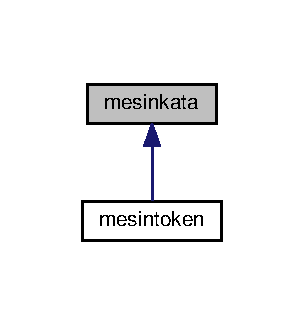
\includegraphics[width=146pt]{classmesinkata__inherit__graph}
\end{center}
\end{figure}
\subsection*{Public Member Functions}
\begin{DoxyCompactItemize}
\item 
\hyperlink{classmesinkata_a0ecf4ed898251dd6a05e11744090881e}{mesinkata} ()
\item 
\hyperlink{classmesinkata_a7cedc728dcc5bf339066dd2aae1c9f58}{mesinkata} (const std\-::string \&\-\_\-pitakar)
\item 
\hyperlink{classmesinkata_a0d221316d72f1bdfcdf4bd8eb11a5d91}{mesinkata} (const \hyperlink{classmesinkata}{mesinkata} \&m)
\item 
\hyperlink{classmesinkata_ad37a3e30b664e6092c0273c66148bf7d}{$\sim$mesinkata} ()
\item 
\hyperlink{classmesinkata}{mesinkata} \& \hyperlink{classmesinkata_a7bcafd23d907196725a133342ca7c99d}{operator=} (const \hyperlink{classmesinkata}{mesinkata} \&m)
\item 
std\-::string \hyperlink{classmesinkata_aa87c5d5fd7f0c45cce2244e3d80492e9}{Get\-Kata} () const 
\item 
bool \hyperlink{classmesinkata_a608feb73de0532ebcd4f3a079054b87d}{Get\-End} () const 
\item 
void \hyperlink{classmesinkata_ac09172015c4a048cb429198988a95472}{Set\-Pita\-Karakter} (const std\-::string \&\-\_\-pitakar)
\item 
void \hyperlink{classmesinkata_ab0628c8aa28428f280ddddc3fbbb5625}{Set\-Kata} (const std\-::string \&S\-T)
\item 
void \hyperlink{classmesinkata_ade4e0c75e5844ea47e8530a2b8ecacb9}{Set\-End} (bool End)
\item 
void \hyperlink{classmesinkata_a016945f311dfbb8c049dd5f9f6b0c852}{Ignore\-\_\-\-Blank} ()
\item 
void \hyperlink{classmesinkata_a9ce4e2f76886ae5674bdd02c395ad9c4}{S\-T\-A\-R\-T} ()
\item 
void \hyperlink{classmesinkata_aa9d334f1b013d6e2f23f791346561e76}{A\-D\-V} ()
\begin{DoxyCompactList}\small\item\em memulai pembacaan \end{DoxyCompactList}\item 
void \hyperlink{classmesinkata_a59ea3cc863b68a69bd728715242fef55}{Salin\-Kata} ()
\begin{DoxyCompactList}\small\item\em maju satu kata. prekondisi\-: !\-End() \end{DoxyCompactList}\item 
\hyperlink{classmesinkata_a0ecf4ed898251dd6a05e11744090881e}{mesinkata} ()
\item 
\hyperlink{classmesinkata_a7cedc728dcc5bf339066dd2aae1c9f58}{mesinkata} (const std\-::string \&\-\_\-pitakar)
\item 
\hyperlink{classmesinkata_a0d221316d72f1bdfcdf4bd8eb11a5d91}{mesinkata} (const \hyperlink{classmesinkata}{mesinkata} \&m)
\item 
\hyperlink{classmesinkata_ad37a3e30b664e6092c0273c66148bf7d}{$\sim$mesinkata} ()
\item 
\hyperlink{classmesinkata}{mesinkata} \& \hyperlink{classmesinkata_ad9dd839515c249890f5209c6223a71b6}{operator=} (const \hyperlink{classmesinkata}{mesinkata} \&m)
\item 
std\-::string \hyperlink{classmesinkata_aa87c5d5fd7f0c45cce2244e3d80492e9}{Get\-Kata} () const 
\item 
bool \hyperlink{classmesinkata_a608feb73de0532ebcd4f3a079054b87d}{Get\-End} () const 
\item 
void \hyperlink{classmesinkata_ac09172015c4a048cb429198988a95472}{Set\-Pita\-Karakter} (const std\-::string \&\-\_\-pitakar)
\item 
void \hyperlink{classmesinkata_ab0628c8aa28428f280ddddc3fbbb5625}{Set\-Kata} (const std\-::string \&S\-T)
\item 
void \hyperlink{classmesinkata_ade4e0c75e5844ea47e8530a2b8ecacb9}{Set\-End} (bool End)
\item 
void \hyperlink{classmesinkata_a016945f311dfbb8c049dd5f9f6b0c852}{Ignore\-\_\-\-Blank} ()
\item 
void \hyperlink{classmesinkata_a9ce4e2f76886ae5674bdd02c395ad9c4}{S\-T\-A\-R\-T} ()
\item 
void \hyperlink{classmesinkata_aa9d334f1b013d6e2f23f791346561e76}{A\-D\-V} ()
\begin{DoxyCompactList}\small\item\em memulai pembacaan \end{DoxyCompactList}\item 
void \hyperlink{classmesinkata_a59ea3cc863b68a69bd728715242fef55}{Salin\-Kata} ()
\begin{DoxyCompactList}\small\item\em maju satu kata. prekondisi\-: !\-End() \end{DoxyCompactList}\end{DoxyCompactItemize}


\subsection{Detailed Description}
kelas mesin kata, cara menggunakan\-: konstruksi, set pita karakter, lalu for(start();!\-End();\hyperlink{classmesinkata_aa9d334f1b013d6e2f23f791346561e76}{A\-D\-V()}) 

\subsection{Constructor \& Destructor Documentation}
\hypertarget{classmesinkata_a0ecf4ed898251dd6a05e11744090881e}{\index{mesinkata@{mesinkata}!mesinkata@{mesinkata}}
\index{mesinkata@{mesinkata}!mesinkata@{mesinkata}}
\subsubsection[{mesinkata}]{\setlength{\rightskip}{0pt plus 5cm}mesinkata\-::mesinkata (
\begin{DoxyParamCaption}
{}
\end{DoxyParamCaption}
)}}\label{classmesinkata_a0ecf4ed898251dd6a05e11744090881e}
\hypertarget{classmesinkata_a7cedc728dcc5bf339066dd2aae1c9f58}{\index{mesinkata@{mesinkata}!mesinkata@{mesinkata}}
\index{mesinkata@{mesinkata}!mesinkata@{mesinkata}}
\subsubsection[{mesinkata}]{\setlength{\rightskip}{0pt plus 5cm}mesinkata\-::mesinkata (
\begin{DoxyParamCaption}
\item[{const std\-::string \&}]{\-\_\-pitakar}
\end{DoxyParamCaption}
)}}\label{classmesinkata_a7cedc728dcc5bf339066dd2aae1c9f58}
\hypertarget{classmesinkata_a0d221316d72f1bdfcdf4bd8eb11a5d91}{\index{mesinkata@{mesinkata}!mesinkata@{mesinkata}}
\index{mesinkata@{mesinkata}!mesinkata@{mesinkata}}
\subsubsection[{mesinkata}]{\setlength{\rightskip}{0pt plus 5cm}mesinkata\-::mesinkata (
\begin{DoxyParamCaption}
\item[{const {\bf mesinkata} \&}]{m}
\end{DoxyParamCaption}
)}}\label{classmesinkata_a0d221316d72f1bdfcdf4bd8eb11a5d91}
\hypertarget{classmesinkata_ad37a3e30b664e6092c0273c66148bf7d}{\index{mesinkata@{mesinkata}!$\sim$mesinkata@{$\sim$mesinkata}}
\index{$\sim$mesinkata@{$\sim$mesinkata}!mesinkata@{mesinkata}}
\subsubsection[{$\sim$mesinkata}]{\setlength{\rightskip}{0pt plus 5cm}mesinkata\-::$\sim$mesinkata (
\begin{DoxyParamCaption}
{}
\end{DoxyParamCaption}
)}}\label{classmesinkata_ad37a3e30b664e6092c0273c66148bf7d}
\hypertarget{classmesinkata_a0ecf4ed898251dd6a05e11744090881e}{\index{mesinkata@{mesinkata}!mesinkata@{mesinkata}}
\index{mesinkata@{mesinkata}!mesinkata@{mesinkata}}
\subsubsection[{mesinkata}]{\setlength{\rightskip}{0pt plus 5cm}mesinkata\-::mesinkata (
\begin{DoxyParamCaption}
{}
\end{DoxyParamCaption}
)}}\label{classmesinkata_a0ecf4ed898251dd6a05e11744090881e}
\hypertarget{classmesinkata_a7cedc728dcc5bf339066dd2aae1c9f58}{\index{mesinkata@{mesinkata}!mesinkata@{mesinkata}}
\index{mesinkata@{mesinkata}!mesinkata@{mesinkata}}
\subsubsection[{mesinkata}]{\setlength{\rightskip}{0pt plus 5cm}mesinkata\-::mesinkata (
\begin{DoxyParamCaption}
\item[{const std\-::string \&}]{\-\_\-pitakar}
\end{DoxyParamCaption}
)}}\label{classmesinkata_a7cedc728dcc5bf339066dd2aae1c9f58}
\hypertarget{classmesinkata_a0d221316d72f1bdfcdf4bd8eb11a5d91}{\index{mesinkata@{mesinkata}!mesinkata@{mesinkata}}
\index{mesinkata@{mesinkata}!mesinkata@{mesinkata}}
\subsubsection[{mesinkata}]{\setlength{\rightskip}{0pt plus 5cm}mesinkata\-::mesinkata (
\begin{DoxyParamCaption}
\item[{const {\bf mesinkata} \&}]{m}
\end{DoxyParamCaption}
)}}\label{classmesinkata_a0d221316d72f1bdfcdf4bd8eb11a5d91}
\hypertarget{classmesinkata_ad37a3e30b664e6092c0273c66148bf7d}{\index{mesinkata@{mesinkata}!$\sim$mesinkata@{$\sim$mesinkata}}
\index{$\sim$mesinkata@{$\sim$mesinkata}!mesinkata@{mesinkata}}
\subsubsection[{$\sim$mesinkata}]{\setlength{\rightskip}{0pt plus 5cm}mesinkata\-::$\sim$mesinkata (
\begin{DoxyParamCaption}
{}
\end{DoxyParamCaption}
)}}\label{classmesinkata_ad37a3e30b664e6092c0273c66148bf7d}


\subsection{Member Function Documentation}
\hypertarget{classmesinkata_aa9d334f1b013d6e2f23f791346561e76}{\index{mesinkata@{mesinkata}!A\-D\-V@{A\-D\-V}}
\index{A\-D\-V@{A\-D\-V}!mesinkata@{mesinkata}}
\subsubsection[{A\-D\-V}]{\setlength{\rightskip}{0pt plus 5cm}void mesinkata\-::\-A\-D\-V (
\begin{DoxyParamCaption}
{}
\end{DoxyParamCaption}
)}}\label{classmesinkata_aa9d334f1b013d6e2f23f791346561e76}


memulai pembacaan 

\hypertarget{classmesinkata_aa9d334f1b013d6e2f23f791346561e76}{\index{mesinkata@{mesinkata}!A\-D\-V@{A\-D\-V}}
\index{A\-D\-V@{A\-D\-V}!mesinkata@{mesinkata}}
\subsubsection[{A\-D\-V}]{\setlength{\rightskip}{0pt plus 5cm}void mesinkata\-::\-A\-D\-V (
\begin{DoxyParamCaption}
{}
\end{DoxyParamCaption}
)}}\label{classmesinkata_aa9d334f1b013d6e2f23f791346561e76}


memulai pembacaan 

\hypertarget{classmesinkata_a608feb73de0532ebcd4f3a079054b87d}{\index{mesinkata@{mesinkata}!Get\-End@{Get\-End}}
\index{Get\-End@{Get\-End}!mesinkata@{mesinkata}}
\subsubsection[{Get\-End}]{\setlength{\rightskip}{0pt plus 5cm}bool mesinkata\-::\-Get\-End (
\begin{DoxyParamCaption}
{}
\end{DoxyParamCaption}
) const}}\label{classmesinkata_a608feb73de0532ebcd4f3a079054b87d}
\hypertarget{classmesinkata_a608feb73de0532ebcd4f3a079054b87d}{\index{mesinkata@{mesinkata}!Get\-End@{Get\-End}}
\index{Get\-End@{Get\-End}!mesinkata@{mesinkata}}
\subsubsection[{Get\-End}]{\setlength{\rightskip}{0pt plus 5cm}bool mesinkata\-::\-Get\-End (
\begin{DoxyParamCaption}
{}
\end{DoxyParamCaption}
) const}}\label{classmesinkata_a608feb73de0532ebcd4f3a079054b87d}
\hypertarget{classmesinkata_aa87c5d5fd7f0c45cce2244e3d80492e9}{\index{mesinkata@{mesinkata}!Get\-Kata@{Get\-Kata}}
\index{Get\-Kata@{Get\-Kata}!mesinkata@{mesinkata}}
\subsubsection[{Get\-Kata}]{\setlength{\rightskip}{0pt plus 5cm}std\-::string mesinkata\-::\-Get\-Kata (
\begin{DoxyParamCaption}
{}
\end{DoxyParamCaption}
) const}}\label{classmesinkata_aa87c5d5fd7f0c45cce2244e3d80492e9}
\hypertarget{classmesinkata_aa87c5d5fd7f0c45cce2244e3d80492e9}{\index{mesinkata@{mesinkata}!Get\-Kata@{Get\-Kata}}
\index{Get\-Kata@{Get\-Kata}!mesinkata@{mesinkata}}
\subsubsection[{Get\-Kata}]{\setlength{\rightskip}{0pt plus 5cm}std\-::string mesinkata\-::\-Get\-Kata (
\begin{DoxyParamCaption}
{}
\end{DoxyParamCaption}
) const}}\label{classmesinkata_aa87c5d5fd7f0c45cce2244e3d80492e9}
\hypertarget{classmesinkata_a016945f311dfbb8c049dd5f9f6b0c852}{\index{mesinkata@{mesinkata}!Ignore\-\_\-\-Blank@{Ignore\-\_\-\-Blank}}
\index{Ignore\-\_\-\-Blank@{Ignore\-\_\-\-Blank}!mesinkata@{mesinkata}}
\subsubsection[{Ignore\-\_\-\-Blank}]{\setlength{\rightskip}{0pt plus 5cm}void mesinkata\-::\-Ignore\-\_\-\-Blank (
\begin{DoxyParamCaption}
{}
\end{DoxyParamCaption}
)}}\label{classmesinkata_a016945f311dfbb8c049dd5f9f6b0c852}
\hypertarget{classmesinkata_a016945f311dfbb8c049dd5f9f6b0c852}{\index{mesinkata@{mesinkata}!Ignore\-\_\-\-Blank@{Ignore\-\_\-\-Blank}}
\index{Ignore\-\_\-\-Blank@{Ignore\-\_\-\-Blank}!mesinkata@{mesinkata}}
\subsubsection[{Ignore\-\_\-\-Blank}]{\setlength{\rightskip}{0pt plus 5cm}void mesinkata\-::\-Ignore\-\_\-\-Blank (
\begin{DoxyParamCaption}
{}
\end{DoxyParamCaption}
)}}\label{classmesinkata_a016945f311dfbb8c049dd5f9f6b0c852}
\hypertarget{classmesinkata_a7bcafd23d907196725a133342ca7c99d}{\index{mesinkata@{mesinkata}!operator=@{operator=}}
\index{operator=@{operator=}!mesinkata@{mesinkata}}
\subsubsection[{operator=}]{\setlength{\rightskip}{0pt plus 5cm}{\bf mesinkata} \& mesinkata\-::operator= (
\begin{DoxyParamCaption}
\item[{const {\bf mesinkata} \&}]{m}
\end{DoxyParamCaption}
)}}\label{classmesinkata_a7bcafd23d907196725a133342ca7c99d}
\hypertarget{classmesinkata_ad9dd839515c249890f5209c6223a71b6}{\index{mesinkata@{mesinkata}!operator=@{operator=}}
\index{operator=@{operator=}!mesinkata@{mesinkata}}
\subsubsection[{operator=}]{\setlength{\rightskip}{0pt plus 5cm}{\bf mesinkata}\& mesinkata\-::operator= (
\begin{DoxyParamCaption}
\item[{const {\bf mesinkata} \&}]{m}
\end{DoxyParamCaption}
)}}\label{classmesinkata_ad9dd839515c249890f5209c6223a71b6}
\hypertarget{classmesinkata_a59ea3cc863b68a69bd728715242fef55}{\index{mesinkata@{mesinkata}!Salin\-Kata@{Salin\-Kata}}
\index{Salin\-Kata@{Salin\-Kata}!mesinkata@{mesinkata}}
\subsubsection[{Salin\-Kata}]{\setlength{\rightskip}{0pt plus 5cm}void mesinkata\-::\-Salin\-Kata (
\begin{DoxyParamCaption}
{}
\end{DoxyParamCaption}
)}}\label{classmesinkata_a59ea3cc863b68a69bd728715242fef55}


maju satu kata. prekondisi\-: !\-End() 

\hypertarget{classmesinkata_a59ea3cc863b68a69bd728715242fef55}{\index{mesinkata@{mesinkata}!Salin\-Kata@{Salin\-Kata}}
\index{Salin\-Kata@{Salin\-Kata}!mesinkata@{mesinkata}}
\subsubsection[{Salin\-Kata}]{\setlength{\rightskip}{0pt plus 5cm}void mesinkata\-::\-Salin\-Kata (
\begin{DoxyParamCaption}
{}
\end{DoxyParamCaption}
)}}\label{classmesinkata_a59ea3cc863b68a69bd728715242fef55}


maju satu kata. prekondisi\-: !\-End() 

\hypertarget{classmesinkata_ade4e0c75e5844ea47e8530a2b8ecacb9}{\index{mesinkata@{mesinkata}!Set\-End@{Set\-End}}
\index{Set\-End@{Set\-End}!mesinkata@{mesinkata}}
\subsubsection[{Set\-End}]{\setlength{\rightskip}{0pt plus 5cm}void mesinkata\-::\-Set\-End (
\begin{DoxyParamCaption}
\item[{bool}]{End}
\end{DoxyParamCaption}
)}}\label{classmesinkata_ade4e0c75e5844ea47e8530a2b8ecacb9}
\hypertarget{classmesinkata_ade4e0c75e5844ea47e8530a2b8ecacb9}{\index{mesinkata@{mesinkata}!Set\-End@{Set\-End}}
\index{Set\-End@{Set\-End}!mesinkata@{mesinkata}}
\subsubsection[{Set\-End}]{\setlength{\rightskip}{0pt plus 5cm}void mesinkata\-::\-Set\-End (
\begin{DoxyParamCaption}
\item[{bool}]{End}
\end{DoxyParamCaption}
)}}\label{classmesinkata_ade4e0c75e5844ea47e8530a2b8ecacb9}
\hypertarget{classmesinkata_ab0628c8aa28428f280ddddc3fbbb5625}{\index{mesinkata@{mesinkata}!Set\-Kata@{Set\-Kata}}
\index{Set\-Kata@{Set\-Kata}!mesinkata@{mesinkata}}
\subsubsection[{Set\-Kata}]{\setlength{\rightskip}{0pt plus 5cm}void mesinkata\-::\-Set\-Kata (
\begin{DoxyParamCaption}
\item[{const std\-::string \&}]{S\-T}
\end{DoxyParamCaption}
)}}\label{classmesinkata_ab0628c8aa28428f280ddddc3fbbb5625}
\hypertarget{classmesinkata_ab0628c8aa28428f280ddddc3fbbb5625}{\index{mesinkata@{mesinkata}!Set\-Kata@{Set\-Kata}}
\index{Set\-Kata@{Set\-Kata}!mesinkata@{mesinkata}}
\subsubsection[{Set\-Kata}]{\setlength{\rightskip}{0pt plus 5cm}void mesinkata\-::\-Set\-Kata (
\begin{DoxyParamCaption}
\item[{const std\-::string \&}]{S\-T}
\end{DoxyParamCaption}
)}}\label{classmesinkata_ab0628c8aa28428f280ddddc3fbbb5625}
\hypertarget{classmesinkata_ac09172015c4a048cb429198988a95472}{\index{mesinkata@{mesinkata}!Set\-Pita\-Karakter@{Set\-Pita\-Karakter}}
\index{Set\-Pita\-Karakter@{Set\-Pita\-Karakter}!mesinkata@{mesinkata}}
\subsubsection[{Set\-Pita\-Karakter}]{\setlength{\rightskip}{0pt plus 5cm}void mesinkata\-::\-Set\-Pita\-Karakter (
\begin{DoxyParamCaption}
\item[{const std\-::string \&}]{\-\_\-pitakar}
\end{DoxyParamCaption}
)}}\label{classmesinkata_ac09172015c4a048cb429198988a95472}
\hypertarget{classmesinkata_ac09172015c4a048cb429198988a95472}{\index{mesinkata@{mesinkata}!Set\-Pita\-Karakter@{Set\-Pita\-Karakter}}
\index{Set\-Pita\-Karakter@{Set\-Pita\-Karakter}!mesinkata@{mesinkata}}
\subsubsection[{Set\-Pita\-Karakter}]{\setlength{\rightskip}{0pt plus 5cm}void mesinkata\-::\-Set\-Pita\-Karakter (
\begin{DoxyParamCaption}
\item[{const std\-::string \&}]{\-\_\-pitakar}
\end{DoxyParamCaption}
)}}\label{classmesinkata_ac09172015c4a048cb429198988a95472}
\hypertarget{classmesinkata_a9ce4e2f76886ae5674bdd02c395ad9c4}{\index{mesinkata@{mesinkata}!S\-T\-A\-R\-T@{S\-T\-A\-R\-T}}
\index{S\-T\-A\-R\-T@{S\-T\-A\-R\-T}!mesinkata@{mesinkata}}
\subsubsection[{S\-T\-A\-R\-T}]{\setlength{\rightskip}{0pt plus 5cm}void mesinkata\-::\-S\-T\-A\-R\-T (
\begin{DoxyParamCaption}
{}
\end{DoxyParamCaption}
)}}\label{classmesinkata_a9ce4e2f76886ae5674bdd02c395ad9c4}
\hypertarget{classmesinkata_a9ce4e2f76886ae5674bdd02c395ad9c4}{\index{mesinkata@{mesinkata}!S\-T\-A\-R\-T@{S\-T\-A\-R\-T}}
\index{S\-T\-A\-R\-T@{S\-T\-A\-R\-T}!mesinkata@{mesinkata}}
\subsubsection[{S\-T\-A\-R\-T}]{\setlength{\rightskip}{0pt plus 5cm}void mesinkata\-::\-S\-T\-A\-R\-T (
\begin{DoxyParamCaption}
{}
\end{DoxyParamCaption}
)}}\label{classmesinkata_a9ce4e2f76886ae5674bdd02c395ad9c4}


The documentation for this class was generated from the following files\-:\begin{DoxyCompactItemize}
\item 
/home/nim\-\_\-13512501/\-Documents/tubes 1 O\-O\-P/src/katakr/\hyperlink{katakr_2mesinkata_8h}{mesinkata.\-h}\item 
/home/nim\-\_\-13512501/\-Documents/tubes 1 O\-O\-P/src/katakr/\hyperlink{mesinkata_8cpp}{mesinkata.\-cpp}\end{DoxyCompactItemize}

\hypertarget{classmesintoken}{\section{mesintoken Class Reference}
\label{classmesintoken}\index{mesintoken@{mesintoken}}
}


{\ttfamily \#include $<$mesintoken.\-h$>$}



Inheritance diagram for mesintoken\-:\nopagebreak
\begin{figure}[H]
\begin{center}
\leavevmode
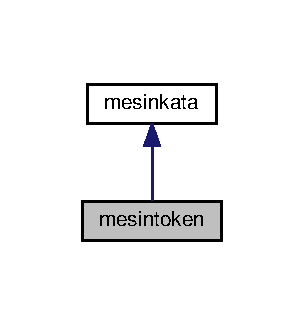
\includegraphics[width=146pt]{classmesintoken__inherit__graph}
\end{center}
\end{figure}


Collaboration diagram for mesintoken\-:\nopagebreak
\begin{figure}[H]
\begin{center}
\leavevmode
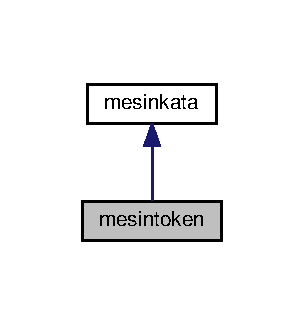
\includegraphics[width=146pt]{classmesintoken__coll__graph}
\end{center}
\end{figure}
\subsection*{Public Member Functions}
\begin{DoxyCompactItemize}
\item 
\hyperlink{classmesintoken_aecc28dabdb54b87985b0ccd62f119f8f}{mesintoken} (const std\-::string \&S\-T)
\begin{DoxyCompactList}\small\item\em membentuk mesin token dengan pita karakter S\-T \end{DoxyCompactList}\item 
\hyperlink{classmesintoken_a36904a5bfe632c649790f47626ecd6cb}{mesintoken} (const std\-::string \&S\-T, const \hyperlink{class_converter}{Converter} \&\-\_\-cvt)
\begin{DoxyCompactList}\small\item\em membentuk mesin token dengan pita karakter S\-T dan converter cvt \end{DoxyCompactList}\end{DoxyCompactItemize}
{\bf }\par
\begin{DoxyCompactItemize}
\item 
\hyperlink{class_token}{Token} \hyperlink{classmesintoken_a996213e867abc8a7f20a06630df9ab89}{Get\-C\-Token} () const 
\end{DoxyCompactItemize}

\begin{Indent}{\bf override\textbackslash{}n}\par
{\em method-\/method ini mengoverride dengan menambahkan konversi ke token dan disimpan di C\-Token

prekondisi pita karakter tidak kosong }\begin{DoxyCompactItemize}
\item 
void \hyperlink{classmesintoken_a1a5b2f1c7ddd5f763a8f94d8e1c7a37c}{S\-T\-A\-R\-T} ()
\item 
void \hyperlink{classmesintoken_affa342e1600ea0fa9e6d6f40cd76919e}{A\-D\-V} ()
\begin{DoxyCompactList}\small\item\em prekondisi\-: !\-Get\-End() \end{DoxyCompactList}\end{DoxyCompactItemize}
\end{Indent}


\subsection{Detailed Description}
tidak bisa untuk polymorphism\par
virtual destruktor belum diimplementasi (tidak dibutuhkan untuk proyek ini)\par
Responsibility\par
Membaca ekspresi token per token\par
Kelas ini menggunakan std\-::string. Kelas ini mewarisi Mesin Kata. Kelas ini mengandung kelas converter.\par
Method kelas ini meliputi konstruktor yang menerima string pita karakter, \hyperlink{classmesintoken_a1a5b2f1c7ddd5f763a8f94d8e1c7a37c}{S\-T\-A\-R\-T()}, \hyperlink{classmesintoken_affa342e1600ea0fa9e6d6f40cd76919e}{A\-D\-V()}, \hyperlink{classmesintoken_a996213e867abc8a7f20a06630df9ab89}{Get\-C\-Token()}. Start memulai mesin, A\-D\-V memajukan satu token, dan \hyperlink{classmesintoken_a996213e867abc8a7f20a06630df9ab89}{Get\-C\-Token()} mengakses token yang sedang dibaca.\par
 

\subsection{Constructor \& Destructor Documentation}
\hypertarget{classmesintoken_aecc28dabdb54b87985b0ccd62f119f8f}{\index{mesintoken@{mesintoken}!mesintoken@{mesintoken}}
\index{mesintoken@{mesintoken}!mesintoken@{mesintoken}}
\subsubsection[{mesintoken}]{\setlength{\rightskip}{0pt plus 5cm}mesintoken\-::mesintoken (
\begin{DoxyParamCaption}
\item[{const std\-::string \&}]{S\-T}
\end{DoxyParamCaption}
)}}\label{classmesintoken_aecc28dabdb54b87985b0ccd62f119f8f}


membentuk mesin token dengan pita karakter S\-T 

\hypertarget{classmesintoken_a36904a5bfe632c649790f47626ecd6cb}{\index{mesintoken@{mesintoken}!mesintoken@{mesintoken}}
\index{mesintoken@{mesintoken}!mesintoken@{mesintoken}}
\subsubsection[{mesintoken}]{\setlength{\rightskip}{0pt plus 5cm}mesintoken\-::mesintoken (
\begin{DoxyParamCaption}
\item[{const std\-::string \&}]{S\-T, }
\item[{const {\bf Converter} \&}]{\-\_\-cvt}
\end{DoxyParamCaption}
)}}\label{classmesintoken_a36904a5bfe632c649790f47626ecd6cb}


membentuk mesin token dengan pita karakter S\-T dan converter cvt 



\subsection{Member Function Documentation}
\hypertarget{classmesintoken_affa342e1600ea0fa9e6d6f40cd76919e}{\index{mesintoken@{mesintoken}!A\-D\-V@{A\-D\-V}}
\index{A\-D\-V@{A\-D\-V}!mesintoken@{mesintoken}}
\subsubsection[{A\-D\-V}]{\setlength{\rightskip}{0pt plus 5cm}void mesintoken\-::\-A\-D\-V (
\begin{DoxyParamCaption}
{}
\end{DoxyParamCaption}
)}}\label{classmesintoken_affa342e1600ea0fa9e6d6f40cd76919e}


prekondisi\-: !\-Get\-End() 

\hypertarget{classmesintoken_a996213e867abc8a7f20a06630df9ab89}{\index{mesintoken@{mesintoken}!Get\-C\-Token@{Get\-C\-Token}}
\index{Get\-C\-Token@{Get\-C\-Token}!mesintoken@{mesintoken}}
\subsubsection[{Get\-C\-Token}]{\setlength{\rightskip}{0pt plus 5cm}{\bf Token} mesintoken\-::\-Get\-C\-Token (
\begin{DoxyParamCaption}
{}
\end{DoxyParamCaption}
) const}}\label{classmesintoken_a996213e867abc8a7f20a06630df9ab89}
Getter prekondisi\-: !\-Get\-End() \hypertarget{classmesintoken_a1a5b2f1c7ddd5f763a8f94d8e1c7a37c}{\index{mesintoken@{mesintoken}!S\-T\-A\-R\-T@{S\-T\-A\-R\-T}}
\index{S\-T\-A\-R\-T@{S\-T\-A\-R\-T}!mesintoken@{mesintoken}}
\subsubsection[{S\-T\-A\-R\-T}]{\setlength{\rightskip}{0pt plus 5cm}void mesintoken\-::\-S\-T\-A\-R\-T (
\begin{DoxyParamCaption}
{}
\end{DoxyParamCaption}
)}}\label{classmesintoken_a1a5b2f1c7ddd5f763a8f94d8e1c7a37c}


The documentation for this class was generated from the following files\-:\begin{DoxyCompactItemize}
\item 
/home/nim\-\_\-13512501/\-Documents/tubes 1 O\-O\-P/src/token/\hyperlink{mesintoken_8h}{mesintoken.\-h}\item 
/home/nim\-\_\-13512501/\-Documents/tubes 1 O\-O\-P/src/token/\hyperlink{mesintoken_8cpp}{mesintoken.\-cpp}\end{DoxyCompactItemize}

\hypertarget{class_operator}{\section{Operator Class Reference}
\label{class_operator}\index{Operator@{Operator}}
}


{\ttfamily \#include $<$Operator.\-h$>$}



Inheritance diagram for Operator\-:\nopagebreak
\begin{figure}[H]
\begin{center}
\leavevmode
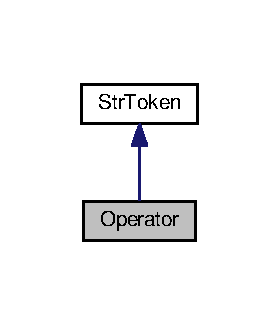
\includegraphics[width=134pt]{class_operator__inherit__graph}
\end{center}
\end{figure}


Collaboration diagram for Operator\-:\nopagebreak
\begin{figure}[H]
\begin{center}
\leavevmode
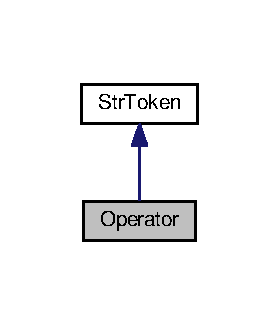
\includegraphics[width=134pt]{class_operator__coll__graph}
\end{center}
\end{figure}
\subsection*{Public Member Functions}
\begin{DoxyCompactItemize}
\item 
\hyperlink{class_operator_acf2514c5e9f48b0a988c955a7d41c486}{Operator} ()
\item 
bool \hyperlink{class_operator_a1b88904a14779cfc05d2337fb2104ab7}{Str\-Rep\-Complies} (const std\-::string \&s)
\begin{DoxyCompactList}\small\item\em mengembalikan true bila s dapat digunakan sebagai representasi operator \end{DoxyCompactList}\item 
void \hyperlink{class_operator_a74ea7dd97fd540327028b19fd84badc9}{Set\-String} (\hyperlink{_token_8h_a29ea73031d51befacf649fa6af865e30}{Tipe\-Token} \-\_\-tkn, const std\-::string \&s)
\item 
std\-::string \hyperlink{class_operator_aad8b367d21ec5508d0ae10ca59adca73}{Get\-String} (\hyperlink{_token_8h_a29ea73031d51befacf649fa6af865e30}{Tipe\-Token} \-\_\-tkn)
\item 
virtual bool \hyperlink{class_operator_a45e663ede5c21432e883db8504b81f86}{can\-Convert} (const std\-::string \&s)
\begin{DoxyCompactList}\small\item\em mengembalikan true bila s dapat dikonversi ke token \end{DoxyCompactList}\item 
virtual std\-::string \hyperlink{class_operator_a1e41cc6d646b1703c7858282cbcf350f}{to\-String} (const \hyperlink{class_token}{Token} \&T)
\begin{DoxyCompactList}\small\item\em mengembalikan representasi string dari token T \end{DoxyCompactList}\item 
virtual \hyperlink{class_token}{Token} \hyperlink{class_operator_a7059095d7977dbdda3068f506b6ed70a}{to\-Token} (const std\-::string \&s)
\begin{DoxyCompactList}\small\item\em mengembalikan representasi token dari string s \end{DoxyCompactList}\end{DoxyCompactItemize}


\subsection{Detailed Description}
kelas implementasi\par
Kelas ini merupakan implementasi kelas \hyperlink{class_str_token}{Str\-Token} dengan konversi sesuai aturan penulisan operator. 

\subsection{Constructor \& Destructor Documentation}
\hypertarget{class_operator_acf2514c5e9f48b0a988c955a7d41c486}{\index{Operator@{Operator}!Operator@{Operator}}
\index{Operator@{Operator}!Operator@{Operator}}
\subsubsection[{Operator}]{\setlength{\rightskip}{0pt plus 5cm}Operator\-::\-Operator (
\begin{DoxyParamCaption}
{}
\end{DoxyParamCaption}
)}}\label{class_operator_acf2514c5e9f48b0a988c955a7d41c486}


\subsection{Member Function Documentation}
\hypertarget{class_operator_a45e663ede5c21432e883db8504b81f86}{\index{Operator@{Operator}!can\-Convert@{can\-Convert}}
\index{can\-Convert@{can\-Convert}!Operator@{Operator}}
\subsubsection[{can\-Convert}]{\setlength{\rightskip}{0pt plus 5cm}bool Operator\-::can\-Convert (
\begin{DoxyParamCaption}
\item[{const std\-::string \&}]{s}
\end{DoxyParamCaption}
)\hspace{0.3cm}{\ttfamily [virtual]}}}\label{class_operator_a45e663ede5c21432e883db8504b81f86}


mengembalikan true bila s dapat dikonversi ke token 



Implements \hyperlink{class_str_token_acd92c843b3b092c21d5a038c5d336957}{Str\-Token}.

\hypertarget{class_operator_aad8b367d21ec5508d0ae10ca59adca73}{\index{Operator@{Operator}!Get\-String@{Get\-String}}
\index{Get\-String@{Get\-String}!Operator@{Operator}}
\subsubsection[{Get\-String}]{\setlength{\rightskip}{0pt plus 5cm}std\-::string Operator\-::\-Get\-String (
\begin{DoxyParamCaption}
\item[{{\bf Tipe\-Token}}]{\-\_\-tkn}
\end{DoxyParamCaption}
)}}\label{class_operator_aad8b367d21ec5508d0ae10ca59adca73}
mengembalikan Opr\mbox{[}\-\_\-tkn\mbox{]} prekondisi\-: 0$<$=\-\_\-tkn$<$T\-I\-P\-E\-T\-O\-K\-E\-N\-\_\-\-C\-O\-U\-N\-T \hypertarget{class_operator_a74ea7dd97fd540327028b19fd84badc9}{\index{Operator@{Operator}!Set\-String@{Set\-String}}
\index{Set\-String@{Set\-String}!Operator@{Operator}}
\subsubsection[{Set\-String}]{\setlength{\rightskip}{0pt plus 5cm}void Operator\-::\-Set\-String (
\begin{DoxyParamCaption}
\item[{{\bf Tipe\-Token}}]{\-\_\-tkn, }
\item[{const std\-::string \&}]{s}
\end{DoxyParamCaption}
)}}\label{class_operator_a74ea7dd97fd540327028b19fd84badc9}
I.\-S.\-: 0$<$= (int) \-\_\-tkn $<$T\-I\-P\-E\-T\-O\-K\-E\-N\-\_\-\-C\-O\-U\-N\-T s tidak dapat dikonversi oleh \hyperlink{class_arab}{Arab}, \hyperlink{class_romawi}{Romawi}, maupun \hyperlink{class_logika}{Logika} \hypertarget{class_operator_a1b88904a14779cfc05d2337fb2104ab7}{\index{Operator@{Operator}!Str\-Rep\-Complies@{Str\-Rep\-Complies}}
\index{Str\-Rep\-Complies@{Str\-Rep\-Complies}!Operator@{Operator}}
\subsubsection[{Str\-Rep\-Complies}]{\setlength{\rightskip}{0pt plus 5cm}bool Operator\-::\-Str\-Rep\-Complies (
\begin{DoxyParamCaption}
\item[{const std\-::string \&}]{s}
\end{DoxyParamCaption}
)}}\label{class_operator_a1b88904a14779cfc05d2337fb2104ab7}


mengembalikan true bila s dapat digunakan sebagai representasi operator 

\hypertarget{class_operator_a1e41cc6d646b1703c7858282cbcf350f}{\index{Operator@{Operator}!to\-String@{to\-String}}
\index{to\-String@{to\-String}!Operator@{Operator}}
\subsubsection[{to\-String}]{\setlength{\rightskip}{0pt plus 5cm}std\-::string Operator\-::to\-String (
\begin{DoxyParamCaption}
\item[{const {\bf Token} \&}]{T}
\end{DoxyParamCaption}
)\hspace{0.3cm}{\ttfamily [virtual]}}}\label{class_operator_a1e41cc6d646b1703c7858282cbcf350f}


mengembalikan representasi string dari token T 



Implements \hyperlink{class_str_token_a9562cf6aff9cefa7a223d78573755e8e}{Str\-Token}.

\hypertarget{class_operator_a7059095d7977dbdda3068f506b6ed70a}{\index{Operator@{Operator}!to\-Token@{to\-Token}}
\index{to\-Token@{to\-Token}!Operator@{Operator}}
\subsubsection[{to\-Token}]{\setlength{\rightskip}{0pt plus 5cm}{\bf Token} Operator\-::to\-Token (
\begin{DoxyParamCaption}
\item[{const std\-::string \&}]{s}
\end{DoxyParamCaption}
)\hspace{0.3cm}{\ttfamily [virtual]}}}\label{class_operator_a7059095d7977dbdda3068f506b6ed70a}


mengembalikan representasi token dari string s 



Implements \hyperlink{class_str_token_ae3f06fac8d7030218db0d833fae6f773}{Str\-Token}.



The documentation for this class was generated from the following files\-:\begin{DoxyCompactItemize}
\item 
/home/nim\-\_\-13512501/\-Documents/tubes 1 O\-O\-P/src/token/\hyperlink{_operator_8h}{Operator.\-h}\item 
/home/nim\-\_\-13512501/\-Documents/tubes 1 O\-O\-P/src/token/\hyperlink{_operator_8cpp}{Operator.\-cpp}\end{DoxyCompactItemize}

\hypertarget{class_romawi}{\section{Romawi Class Reference}
\label{class_romawi}\index{Romawi@{Romawi}}
}


kelas implementasi \hyperlink{class_str_token}{Str\-Token} dengan aturan representasi bilangan romawi  




{\ttfamily \#include $<$Romawi.\-h$>$}



Inheritance diagram for Romawi\-:\nopagebreak
\begin{figure}[H]
\begin{center}
\leavevmode
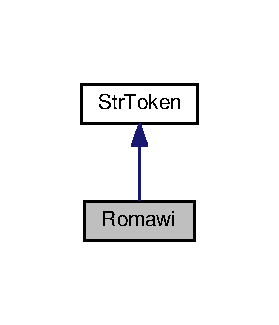
\includegraphics[width=134pt]{class_romawi__inherit__graph}
\end{center}
\end{figure}


Collaboration diagram for Romawi\-:\nopagebreak
\begin{figure}[H]
\begin{center}
\leavevmode
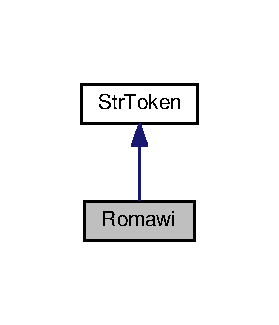
\includegraphics[width=134pt]{class_romawi__coll__graph}
\end{center}
\end{figure}
\subsection*{Public Member Functions}
\begin{DoxyCompactItemize}
\item 
virtual bool \hyperlink{class_romawi_ac99f5ba3d8695bf49d01074bb3afcda3}{can\-Convert} (const std\-::string \&s)
\begin{DoxyCompactList}\small\item\em mengembalikan true bila s dapat dikonversi ke token \end{DoxyCompactList}\item 
virtual std\-::string \hyperlink{class_romawi_ace7c4a68a29912199d4984c71d7f858c}{to\-String} (const \hyperlink{class_token}{Token} \&T)
\begin{DoxyCompactList}\small\item\em mengembalikan representasi string dari token T. \end{DoxyCompactList}\item 
virtual \hyperlink{class_token}{Token} \hyperlink{class_romawi_aacb2db408231ac236b1378f44c501508}{to\-Token} (const std\-::string \&s)
\begin{DoxyCompactList}\small\item\em mengembalikan representasi token dari string s \end{DoxyCompactList}\end{DoxyCompactItemize}


\subsection{Detailed Description}
kelas implementasi \hyperlink{class_str_token}{Str\-Token} dengan aturan representasi bilangan romawi 

\subsection{Member Function Documentation}
\hypertarget{class_romawi_ac99f5ba3d8695bf49d01074bb3afcda3}{\index{Romawi@{Romawi}!can\-Convert@{can\-Convert}}
\index{can\-Convert@{can\-Convert}!Romawi@{Romawi}}
\subsubsection[{can\-Convert}]{\setlength{\rightskip}{0pt plus 5cm}bool Romawi\-::can\-Convert (
\begin{DoxyParamCaption}
\item[{const std\-::string \&}]{s}
\end{DoxyParamCaption}
)\hspace{0.3cm}{\ttfamily [virtual]}}}\label{class_romawi_ac99f5ba3d8695bf49d01074bb3afcda3}


mengembalikan true bila s dapat dikonversi ke token 



Implements \hyperlink{class_str_token_acd92c843b3b092c21d5a038c5d336957}{Str\-Token}.

\hypertarget{class_romawi_ace7c4a68a29912199d4984c71d7f858c}{\index{Romawi@{Romawi}!to\-String@{to\-String}}
\index{to\-String@{to\-String}!Romawi@{Romawi}}
\subsubsection[{to\-String}]{\setlength{\rightskip}{0pt plus 5cm}std\-::string Romawi\-::to\-String (
\begin{DoxyParamCaption}
\item[{const {\bf Token} \&}]{T}
\end{DoxyParamCaption}
)\hspace{0.3cm}{\ttfamily [virtual]}}}\label{class_romawi_ace7c4a68a29912199d4984c71d7f858c}


mengembalikan representasi string dari token T. 



Implements \hyperlink{class_str_token_a9562cf6aff9cefa7a223d78573755e8e}{Str\-Token}.

\hypertarget{class_romawi_aacb2db408231ac236b1378f44c501508}{\index{Romawi@{Romawi}!to\-Token@{to\-Token}}
\index{to\-Token@{to\-Token}!Romawi@{Romawi}}
\subsubsection[{to\-Token}]{\setlength{\rightskip}{0pt plus 5cm}{\bf Token} Romawi\-::to\-Token (
\begin{DoxyParamCaption}
\item[{const std\-::string \&}]{s}
\end{DoxyParamCaption}
)\hspace{0.3cm}{\ttfamily [virtual]}}}\label{class_romawi_aacb2db408231ac236b1378f44c501508}


mengembalikan representasi token dari string s 



Implements \hyperlink{class_str_token_ae3f06fac8d7030218db0d833fae6f773}{Str\-Token}.



The documentation for this class was generated from the following files\-:\begin{DoxyCompactItemize}
\item 
/home/nim\-\_\-13512501/\-Documents/tubes 1 O\-O\-P/src/token/\hyperlink{_romawi_8h}{Romawi.\-h}\item 
/home/nim\-\_\-13512501/\-Documents/tubes 1 O\-O\-P/src/token/\hyperlink{_romawi_8cpp}{Romawi.\-cpp}\end{DoxyCompactItemize}

\hypertarget{class_stack}{\section{Stack$<$ T $>$ Class Template Reference}
\label{class_stack}\index{Stack$<$ T $>$@{Stack$<$ T $>$}}
}


{\ttfamily \#include $<$stack.\-h$>$}

\subsection*{Public Member Functions}
\begin{DoxyCompactItemize}
\item 
\hyperlink{class_stack_aefee698059467258bbd79045aca62a63}{Stack} ()
\begin{DoxyCompactList}\small\item\em Konstruktor. \end{DoxyCompactList}\item 
\hyperlink{class_stack_a8b366aa6e858c1446754e8e39e47bb29}{Stack} (int newsize)
\item 
\hyperlink{class_stack_ac48db567b5a0cbc1b233424584dffaf7}{Stack} (const \hyperlink{class_stack}{Stack} \&S)
\begin{DoxyCompactList}\small\item\em cctor \end{DoxyCompactList}\item 
\hyperlink{class_stack_a9e7a00875aefbdac560ab189b7bc61d1}{$\sim$\-Stack} ()
\item 
\hyperlink{class_stack}{Stack}$<$ T $>$ \& \hyperlink{class_stack_ac9fcee8f3d3c2f444333eb285ced2ad3}{operator=} (const \hyperlink{class_stack}{Stack} \&S)
\begin{DoxyCompactList}\small\item\em assignment \end{DoxyCompactList}\item 
int \hyperlink{class_stack_a536d81ee9a732ad18ab76b84ad5237b2}{Get\-Size} ()
\begin{DoxyCompactList}\small\item\em Getter. \end{DoxyCompactList}\item 
int \hyperlink{class_stack_ad04516610308db3c177b6383d534365f}{Full} ()
\begin{DoxyCompactList}\small\item\em Predikat. \end{DoxyCompactList}\item 
int \hyperlink{class_stack_a30a2b48400dd12a3377dffdaf80024e9}{Empty} ()
\item 
void \hyperlink{class_stack_aacaf0b0e50663caf01f0f6763faa3e10}{Push} (T elemen)
\item 
void \hyperlink{class_stack_ac6535f044f43b47aed7141e2ce502477}{Pop} (T $\ast$elemen)
\end{DoxyCompactItemize}


\subsection{Constructor \& Destructor Documentation}
\hypertarget{class_stack_aefee698059467258bbd79045aca62a63}{\index{Stack@{Stack}!Stack@{Stack}}
\index{Stack@{Stack}!Stack@{Stack}}
\subsubsection[{Stack}]{\setlength{\rightskip}{0pt plus 5cm}template$<$class T $>$ {\bf Stack}$<$ T $>$\-::{\bf Stack} (
\begin{DoxyParamCaption}
{}
\end{DoxyParamCaption}
)}}\label{class_stack_aefee698059467258bbd79045aca62a63}


Konstruktor. 

Implementasi.

Konstruktor \hypertarget{class_stack_a8b366aa6e858c1446754e8e39e47bb29}{\index{Stack@{Stack}!Stack@{Stack}}
\index{Stack@{Stack}!Stack@{Stack}}
\subsubsection[{Stack}]{\setlength{\rightskip}{0pt plus 5cm}template$<$class T $>$ {\bf Stack}$<$ T $>$\-::{\bf Stack} (
\begin{DoxyParamCaption}
\item[{int}]{newsize}
\end{DoxyParamCaption}
)}}\label{class_stack_a8b366aa6e858c1446754e8e39e47bb29}
\hypertarget{class_stack_ac48db567b5a0cbc1b233424584dffaf7}{\index{Stack@{Stack}!Stack@{Stack}}
\index{Stack@{Stack}!Stack@{Stack}}
\subsubsection[{Stack}]{\setlength{\rightskip}{0pt plus 5cm}template$<$class T $>$ {\bf Stack}$<$ T $>$\-::{\bf Stack} (
\begin{DoxyParamCaption}
\item[{const {\bf Stack}$<$ T $>$ \&}]{S}
\end{DoxyParamCaption}
)}}\label{class_stack_ac48db567b5a0cbc1b233424584dffaf7}


cctor 

\hypertarget{class_stack_a9e7a00875aefbdac560ab189b7bc61d1}{\index{Stack@{Stack}!$\sim$\-Stack@{$\sim$\-Stack}}
\index{$\sim$\-Stack@{$\sim$\-Stack}!Stack@{Stack}}
\subsubsection[{$\sim$\-Stack}]{\setlength{\rightskip}{0pt plus 5cm}template$<$class T $>$ {\bf Stack}$<$ T $>$\-::$\sim${\bf Stack} (
\begin{DoxyParamCaption}
{}
\end{DoxyParamCaption}
)}}\label{class_stack_a9e7a00875aefbdac560ab189b7bc61d1}


\subsection{Member Function Documentation}
\hypertarget{class_stack_a30a2b48400dd12a3377dffdaf80024e9}{\index{Stack@{Stack}!Empty@{Empty}}
\index{Empty@{Empty}!Stack@{Stack}}
\subsubsection[{Empty}]{\setlength{\rightskip}{0pt plus 5cm}template$<$class T $>$ int {\bf Stack}$<$ T $>$\-::Empty (
\begin{DoxyParamCaption}
{}
\end{DoxyParamCaption}
)}}\label{class_stack_a30a2b48400dd12a3377dffdaf80024e9}
\hypertarget{class_stack_ad04516610308db3c177b6383d534365f}{\index{Stack@{Stack}!Full@{Full}}
\index{Full@{Full}!Stack@{Stack}}
\subsubsection[{Full}]{\setlength{\rightskip}{0pt plus 5cm}template$<$class T $>$ int {\bf Stack}$<$ T $>$\-::Full (
\begin{DoxyParamCaption}
{}
\end{DoxyParamCaption}
)}}\label{class_stack_ad04516610308db3c177b6383d534365f}


Predikat. 

\hypertarget{class_stack_a536d81ee9a732ad18ab76b84ad5237b2}{\index{Stack@{Stack}!Get\-Size@{Get\-Size}}
\index{Get\-Size@{Get\-Size}!Stack@{Stack}}
\subsubsection[{Get\-Size}]{\setlength{\rightskip}{0pt plus 5cm}template$<$class T $>$ int {\bf Stack}$<$ T $>$\-::Get\-Size (
\begin{DoxyParamCaption}
{}
\end{DoxyParamCaption}
)}}\label{class_stack_a536d81ee9a732ad18ab76b84ad5237b2}


Getter. 

Getter mengembalikan banyaknya elemen yang disimpan di dalam stack \hypertarget{class_stack_ac9fcee8f3d3c2f444333eb285ced2ad3}{\index{Stack@{Stack}!operator=@{operator=}}
\index{operator=@{operator=}!Stack@{Stack}}
\subsubsection[{operator=}]{\setlength{\rightskip}{0pt plus 5cm}template$<$class T $>$ {\bf Stack}$<$ T $>$ \& {\bf Stack}$<$ T $>$\-::operator= (
\begin{DoxyParamCaption}
\item[{const {\bf Stack}$<$ T $>$ \&}]{S}
\end{DoxyParamCaption}
)}}\label{class_stack_ac9fcee8f3d3c2f444333eb285ced2ad3}


assignment 

\hypertarget{class_stack_ac6535f044f43b47aed7141e2ce502477}{\index{Stack@{Stack}!Pop@{Pop}}
\index{Pop@{Pop}!Stack@{Stack}}
\subsubsection[{Pop}]{\setlength{\rightskip}{0pt plus 5cm}template$<$class T$>$ void {\bf Stack}$<$ T $>$\-::Pop (
\begin{DoxyParamCaption}
\item[{T $\ast$}]{elemen}
\end{DoxyParamCaption}
)}}\label{class_stack_ac6535f044f43b47aed7141e2ce502477}
Memasukan elemen ke dalam stack I.\-S \hyperlink{class_stack}{Stack} terdefinisi F.\-S. jika penuh \hyperlink{class_stack}{Stack} akan diresize terlebih dahulu. elemen sudah dimasukan ke dalam stack \hypertarget{class_stack_aacaf0b0e50663caf01f0f6763faa3e10}{\index{Stack@{Stack}!Push@{Push}}
\index{Push@{Push}!Stack@{Stack}}
\subsubsection[{Push}]{\setlength{\rightskip}{0pt plus 5cm}template$<$class T$>$ void {\bf Stack}$<$ T $>$\-::Push (
\begin{DoxyParamCaption}
\item[{T}]{elemen}
\end{DoxyParamCaption}
)}}\label{class_stack_aacaf0b0e50663caf01f0f6763faa3e10}


The documentation for this class was generated from the following file\-:\begin{DoxyCompactItemize}
\item 
/home/nim\-\_\-13512501/\-Documents/tubes 1 O\-O\-P/src/stack/\hyperlink{stack_8h}{stack.\-h}\end{DoxyCompactItemize}

\hypertarget{class_str_token}{\section{Str\-Token Class Reference}
\label{class_str_token}\index{Str\-Token@{Str\-Token}}
}


{\ttfamily \#include $<$Str\-Token.\-h$>$}



Inheritance diagram for Str\-Token\-:\nopagebreak
\begin{figure}[H]
\begin{center}
\leavevmode
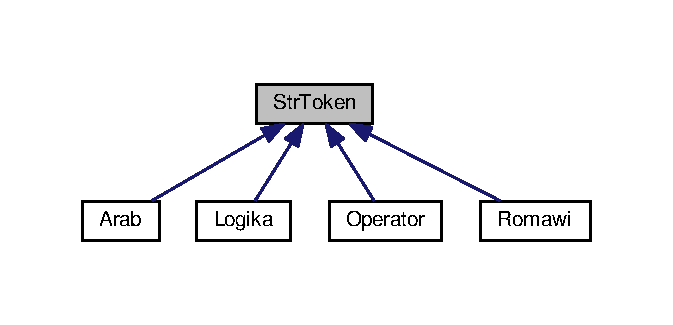
\includegraphics[width=323pt]{class_str_token__inherit__graph}
\end{center}
\end{figure}
\subsection*{Public Member Functions}
\begin{DoxyCompactItemize}
\item 
virtual \hyperlink{class_str_token_a6b1f19d7b05dd697084b743fb1fcf38b}{$\sim$\-Str\-Token} ()
\item 
virtual bool \hyperlink{class_str_token_acd92c843b3b092c21d5a038c5d336957}{can\-Convert} (const std\-::string \&s)=0
\begin{DoxyCompactList}\small\item\em mengembalikan true bila s dapat dikonversi ke token \end{DoxyCompactList}\item 
virtual std\-::string \hyperlink{class_str_token_a9562cf6aff9cefa7a223d78573755e8e}{to\-String} (const \hyperlink{class_token}{Token} \&T)=0
\begin{DoxyCompactList}\small\item\em mengembalikan representasi string dari token T \end{DoxyCompactList}\item 
virtual \hyperlink{class_token}{Token} \hyperlink{class_str_token_ae3f06fac8d7030218db0d833fae6f773}{to\-Token} (const std\-::string \&s)=0
\begin{DoxyCompactList}\small\item\em mengembalikan representasi token dari string s \end{DoxyCompactList}\end{DoxyCompactItemize}


\subsection{Detailed Description}
Responsibility\par
Kelas ini merupakan kelas abstrak. Tanggung jawabnya adalah mengkonversi satu jenis representasi token antara objek string dan token.\par
Hubungan dengan kelas lain\par
kelas ini diimplementasi oleh kelas \hyperlink{class_arab}{Arab}, \hyperlink{class_logika}{Logika}, \hyperlink{class_romawi}{Romawi}, dan \hyperlink{class_operator}{Operator}.\par
Gambaran umum method\par
metodanya adalah mengkonversi dari string ke token dan mengkonversi dari token ke string, serta pengecekan apakah string tertentu dapat dikonversi olehnya\par


\subsection{Constructor \& Destructor Documentation}
\hypertarget{class_str_token_a6b1f19d7b05dd697084b743fb1fcf38b}{\index{Str\-Token@{Str\-Token}!$\sim$\-Str\-Token@{$\sim$\-Str\-Token}}
\index{$\sim$\-Str\-Token@{$\sim$\-Str\-Token}!StrToken@{Str\-Token}}
\subsubsection[{$\sim$\-Str\-Token}]{\setlength{\rightskip}{0pt plus 5cm}virtual Str\-Token\-::$\sim$\-Str\-Token (
\begin{DoxyParamCaption}
{}
\end{DoxyParamCaption}
)\hspace{0.3cm}{\ttfamily [inline]}, {\ttfamily [virtual]}}}\label{class_str_token_a6b1f19d7b05dd697084b743fb1fcf38b}


\subsection{Member Function Documentation}
\hypertarget{class_str_token_acd92c843b3b092c21d5a038c5d336957}{\index{Str\-Token@{Str\-Token}!can\-Convert@{can\-Convert}}
\index{can\-Convert@{can\-Convert}!StrToken@{Str\-Token}}
\subsubsection[{can\-Convert}]{\setlength{\rightskip}{0pt plus 5cm}virtual bool Str\-Token\-::can\-Convert (
\begin{DoxyParamCaption}
\item[{const std\-::string \&}]{s}
\end{DoxyParamCaption}
)\hspace{0.3cm}{\ttfamily [pure virtual]}}}\label{class_str_token_acd92c843b3b092c21d5a038c5d336957}


mengembalikan true bila s dapat dikonversi ke token 



Implemented in \hyperlink{class_operator_a45e663ede5c21432e883db8504b81f86}{Operator}, \hyperlink{class_arab_ab7f0cbcaf9b248b8545b22ccec07a8cd}{Arab}, \hyperlink{class_logika_acb038237bab7f8557b4da5e75eb0ce61}{Logika}, and \hyperlink{class_romawi_ac99f5ba3d8695bf49d01074bb3afcda3}{Romawi}.

\hypertarget{class_str_token_a9562cf6aff9cefa7a223d78573755e8e}{\index{Str\-Token@{Str\-Token}!to\-String@{to\-String}}
\index{to\-String@{to\-String}!StrToken@{Str\-Token}}
\subsubsection[{to\-String}]{\setlength{\rightskip}{0pt plus 5cm}virtual std\-::string Str\-Token\-::to\-String (
\begin{DoxyParamCaption}
\item[{const {\bf Token} \&}]{T}
\end{DoxyParamCaption}
)\hspace{0.3cm}{\ttfamily [pure virtual]}}}\label{class_str_token_a9562cf6aff9cefa7a223d78573755e8e}


mengembalikan representasi string dari token T 



Implemented in \hyperlink{class_operator_a1e41cc6d646b1703c7858282cbcf350f}{Operator}, \hyperlink{class_arab_a097a31788290644f61e76001d7180ec1}{Arab}, \hyperlink{class_logika_accacd24a0d83e98146edd43ab46c789a}{Logika}, and \hyperlink{class_romawi_ace7c4a68a29912199d4984c71d7f858c}{Romawi}.

\hypertarget{class_str_token_ae3f06fac8d7030218db0d833fae6f773}{\index{Str\-Token@{Str\-Token}!to\-Token@{to\-Token}}
\index{to\-Token@{to\-Token}!StrToken@{Str\-Token}}
\subsubsection[{to\-Token}]{\setlength{\rightskip}{0pt plus 5cm}virtual {\bf Token} Str\-Token\-::to\-Token (
\begin{DoxyParamCaption}
\item[{const std\-::string \&}]{s}
\end{DoxyParamCaption}
)\hspace{0.3cm}{\ttfamily [pure virtual]}}}\label{class_str_token_ae3f06fac8d7030218db0d833fae6f773}


mengembalikan representasi token dari string s 



Implemented in \hyperlink{class_operator_a7059095d7977dbdda3068f506b6ed70a}{Operator}, \hyperlink{class_arab_a107f2bde10c4cd4dfd18a44db5739b4c}{Arab}, \hyperlink{class_logika_af52abd9fefcea94bedc313ce61987b3e}{Logika}, and \hyperlink{class_romawi_aacb2db408231ac236b1378f44c501508}{Romawi}.



The documentation for this class was generated from the following file\-:\begin{DoxyCompactItemize}
\item 
/home/nim\-\_\-13512501/\-Documents/tubes 1 O\-O\-P/src/token/\hyperlink{_str_token_8h}{Str\-Token.\-h}\end{DoxyCompactItemize}

\hypertarget{class_token}{\section{Token Class Reference}
\label{class_token}\index{Token@{Token}}
}


{\ttfamily \#include $<$Token.\-h$>$}

\subsection*{Public Member Functions}
\begin{DoxyCompactItemize}
\item 
\hyperlink{class_token_aa3c5868ba4115f3189df6b2ac5b36f39}{Token} ()
\begin{DoxyCompactList}\small\item\em ctor \end{DoxyCompactList}\item 
std\-::string \hyperlink{class_token_aae7b73d9d7cdeaa0a05cc51fbf752e14}{To\-Str} ()
\end{DoxyCompactItemize}
\begin{Indent}{\bf getter}\par
{\em tidak mengubah status token }\begin{DoxyCompactItemize}
\item 
\hyperlink{_token_8h_a29ea73031d51befacf649fa6af865e30}{Tipe\-Token} \hyperlink{class_token_a735a4c2ae32ddce6c8ade6d8ab06f02b}{get\-Tkn} () const 
\begin{DoxyCompactList}\small\item\em mengembalikan tipe token tersebut \end{DoxyCompactList}\item 
\hyperlink{_token_8h_a074bf6c0d33845f3d36e457b9243dcfb}{Tipe} \hyperlink{class_token_af25c1d47e7bf11aa08b1c32aa4920769}{get\-Tipe\-Bilangan} () const 
\begin{DoxyCompactList}\small\item\em prekondisi\-: \hyperlink{class_token_a735a4c2ae32ddce6c8ade6d8ab06f02b}{get\-Tkn()}==Bilangan \end{DoxyCompactList}\item 
int \hyperlink{class_token_aeced03b265a97a1b8cfd557f4613192a}{get\-Bilangan\-Int} () const 
\begin{DoxyCompactList}\small\item\em prekondisi\-: \hyperlink{class_token_af25c1d47e7bf11aa08b1c32aa4920769}{get\-Tipe\-Bilangan()}==\-\_\-int \end{DoxyCompactList}\item 
float \hyperlink{class_token_a32f0323896e15112a72b49bed901cd2e}{get\-Bilangan\-Float} () const 
\begin{DoxyCompactList}\small\item\em prekondisi\-: \hyperlink{class_token_af25c1d47e7bf11aa08b1c32aa4920769}{get\-Tipe\-Bilangan()}==\-\_\-float \end{DoxyCompactList}\item 
bool \hyperlink{class_token_a6ff4b84802344ed9336e27590d7d4b51}{get\-Bilangan\-Bool} () const 
\begin{DoxyCompactList}\small\item\em prekondisi\-: \hyperlink{class_token_af25c1d47e7bf11aa08b1c32aa4920769}{get\-Tipe\-Bilangan()}==\-\_\-bool \end{DoxyCompactList}\end{DoxyCompactItemize}
\end{Indent}
\begin{Indent}{\bf setter}\par
{\em status token. Akan digunakan oleh yang membangun dan mengubah token, seperti converter dan sebagainya }\begin{DoxyCompactItemize}
\item 
void \hyperlink{class_token_ae785baf319454717be06d9ffb11ffd4c}{Set\-Tkn} (\hyperlink{_token_8h_a29ea73031d51befacf649fa6af865e30}{Tipe\-Token} \-\_\-\-Tkn)
\begin{DoxyCompactList}\small\item\em mengeset token \end{DoxyCompactList}\item 
void \hyperlink{class_token_aee9cf292baf9525d39d01edf5d9d7797}{Set\-Bilangan} (float f)
\begin{DoxyCompactList}\small\item\em mengeset bilangan sekaligus tipe token menjadi bilangan dan tipe bilangan menjadi float dan isinya f \end{DoxyCompactList}\item 
void \hyperlink{class_token_ab36a4340c125fc641e319c5261ab13f7}{Set\-Bilangan} (int i)
\begin{DoxyCompactList}\small\item\em mengeset bilangan sekaligus tipe token menjadi bilangan dan tipe bilangan menjadi int dan isinya i \end{DoxyCompactList}\item 
void \hyperlink{class_token_afe10550438e63b07c82f1ab9fac4fd98}{Set\-Bilangan} (bool l)
\begin{DoxyCompactList}\small\item\em mengeset bilangan sekaligus tipe token menjadi bilangan dan tipe bilangan menjadi logika dan isinya l \end{DoxyCompactList}\end{DoxyCompactItemize}
\end{Indent}
\begin{Indent}{\bf predikat}\par
{\em boolean, true false. tidak mengubah status token }\begin{DoxyCompactItemize}
\item 
bool \hyperlink{class_token_a8a15bf44ca4622994dfce8e43f78d76c}{is\-Punctuator} () const 
\begin{DoxyCompactList}\small\item\em mengembalikan true bila ( atau ) \end{DoxyCompactList}\item 
bool \hyperlink{class_token_a08c5aa25effd9d4b7dd5e2dda0f72058}{is\-Opr\-Uner} () const 
\begin{DoxyCompactList}\small\item\em mengembalikan true bila ia operator uner \end{DoxyCompactList}\item 
bool \hyperlink{class_token_aa601738aa08b5ad132d038b0c806fab9}{is\-Opr\-Biner} () const 
\begin{DoxyCompactList}\small\item\em mengembalikan true bila ia operator uner \end{DoxyCompactList}\item 
bool \hyperlink{class_token_a3db1e9f877edcdc5f12fdea1496e7526}{is\-Bilangan} () const 
\begin{DoxyCompactList}\small\item\em mengembalikan true bila token merupakan bilangan \end{DoxyCompactList}\item 
bool \hyperlink{class_token_a40f66005d5df3d37c679258f2c9ab796}{is\-Smaller\-Precedence\-Than} (const \hyperlink{class_token}{Token} \&T)
\end{DoxyCompactItemize}
\end{Indent}
\begin{Indent}{\bf method lain}\par
{\em untuk digunakan oleh kalkulator atau evaluator\par
saat dioperasikan, tipe bilangan dapat berubah\par
}\begin{DoxyCompactItemize}
\item 
\hyperlink{class_token}{Token} \hyperlink{class_token_a7e04e49806d087cbc8062bafe848e471}{Operasikan} (const \hyperlink{class_token}{Token} \&lhs, const \hyperlink{class_token}{Token} \&rhs) const 
\item 
\hyperlink{class_token}{Token} \hyperlink{class_token_ace8d206103c7cd6bda80c9f2beea462b}{Operasikan} (const \hyperlink{class_token}{Token} \&rhs) const 
\end{DoxyCompactItemize}
\end{Indent}


\subsection{Detailed Description}
Kelas token bertanggung jawab sebagai objek yang dapat dimengerti oleh evaluator. Kelas token bertanggung jawab atas jenis-\/jenis bilangan dan operator serta perilakunya perilaku operator yaitu presedensi serta bagaimana operator tersebut mengoperasikan operand 

\subsection{Constructor \& Destructor Documentation}
\hypertarget{class_token_aa3c5868ba4115f3189df6b2ac5b36f39}{\index{Token@{Token}!Token@{Token}}
\index{Token@{Token}!Token@{Token}}
\subsubsection[{Token}]{\setlength{\rightskip}{0pt plus 5cm}Token\-::\-Token (
\begin{DoxyParamCaption}
{}
\end{DoxyParamCaption}
)}}\label{class_token_aa3c5868ba4115f3189df6b2ac5b36f39}


ctor 



\subsection{Member Function Documentation}
\hypertarget{class_token_a6ff4b84802344ed9336e27590d7d4b51}{\index{Token@{Token}!get\-Bilangan\-Bool@{get\-Bilangan\-Bool}}
\index{get\-Bilangan\-Bool@{get\-Bilangan\-Bool}!Token@{Token}}
\subsubsection[{get\-Bilangan\-Bool}]{\setlength{\rightskip}{0pt plus 5cm}bool Token\-::get\-Bilangan\-Bool (
\begin{DoxyParamCaption}
{}
\end{DoxyParamCaption}
) const}}\label{class_token_a6ff4b84802344ed9336e27590d7d4b51}


prekondisi\-: \hyperlink{class_token_af25c1d47e7bf11aa08b1c32aa4920769}{get\-Tipe\-Bilangan()}==\-\_\-bool 

\hypertarget{class_token_a32f0323896e15112a72b49bed901cd2e}{\index{Token@{Token}!get\-Bilangan\-Float@{get\-Bilangan\-Float}}
\index{get\-Bilangan\-Float@{get\-Bilangan\-Float}!Token@{Token}}
\subsubsection[{get\-Bilangan\-Float}]{\setlength{\rightskip}{0pt plus 5cm}float Token\-::get\-Bilangan\-Float (
\begin{DoxyParamCaption}
{}
\end{DoxyParamCaption}
) const}}\label{class_token_a32f0323896e15112a72b49bed901cd2e}


prekondisi\-: \hyperlink{class_token_af25c1d47e7bf11aa08b1c32aa4920769}{get\-Tipe\-Bilangan()}==\-\_\-float 

\hypertarget{class_token_aeced03b265a97a1b8cfd557f4613192a}{\index{Token@{Token}!get\-Bilangan\-Int@{get\-Bilangan\-Int}}
\index{get\-Bilangan\-Int@{get\-Bilangan\-Int}!Token@{Token}}
\subsubsection[{get\-Bilangan\-Int}]{\setlength{\rightskip}{0pt plus 5cm}int Token\-::get\-Bilangan\-Int (
\begin{DoxyParamCaption}
{}
\end{DoxyParamCaption}
) const}}\label{class_token_aeced03b265a97a1b8cfd557f4613192a}


prekondisi\-: \hyperlink{class_token_af25c1d47e7bf11aa08b1c32aa4920769}{get\-Tipe\-Bilangan()}==\-\_\-int 

\hypertarget{class_token_af25c1d47e7bf11aa08b1c32aa4920769}{\index{Token@{Token}!get\-Tipe\-Bilangan@{get\-Tipe\-Bilangan}}
\index{get\-Tipe\-Bilangan@{get\-Tipe\-Bilangan}!Token@{Token}}
\subsubsection[{get\-Tipe\-Bilangan}]{\setlength{\rightskip}{0pt plus 5cm}{\bf Tipe} Token\-::get\-Tipe\-Bilangan (
\begin{DoxyParamCaption}
{}
\end{DoxyParamCaption}
) const}}\label{class_token_af25c1d47e7bf11aa08b1c32aa4920769}


prekondisi\-: \hyperlink{class_token_a735a4c2ae32ddce6c8ade6d8ab06f02b}{get\-Tkn()}==Bilangan 

\hypertarget{class_token_a735a4c2ae32ddce6c8ade6d8ab06f02b}{\index{Token@{Token}!get\-Tkn@{get\-Tkn}}
\index{get\-Tkn@{get\-Tkn}!Token@{Token}}
\subsubsection[{get\-Tkn}]{\setlength{\rightskip}{0pt plus 5cm}{\bf Tipe\-Token} Token\-::get\-Tkn (
\begin{DoxyParamCaption}
{}
\end{DoxyParamCaption}
) const}}\label{class_token_a735a4c2ae32ddce6c8ade6d8ab06f02b}


mengembalikan tipe token tersebut 

\hypertarget{class_token_a3db1e9f877edcdc5f12fdea1496e7526}{\index{Token@{Token}!is\-Bilangan@{is\-Bilangan}}
\index{is\-Bilangan@{is\-Bilangan}!Token@{Token}}
\subsubsection[{is\-Bilangan}]{\setlength{\rightskip}{0pt plus 5cm}bool Token\-::is\-Bilangan (
\begin{DoxyParamCaption}
{}
\end{DoxyParamCaption}
) const}}\label{class_token_a3db1e9f877edcdc5f12fdea1496e7526}


mengembalikan true bila token merupakan bilangan 

\hypertarget{class_token_aa601738aa08b5ad132d038b0c806fab9}{\index{Token@{Token}!is\-Opr\-Biner@{is\-Opr\-Biner}}
\index{is\-Opr\-Biner@{is\-Opr\-Biner}!Token@{Token}}
\subsubsection[{is\-Opr\-Biner}]{\setlength{\rightskip}{0pt plus 5cm}bool Token\-::is\-Opr\-Biner (
\begin{DoxyParamCaption}
{}
\end{DoxyParamCaption}
) const}}\label{class_token_aa601738aa08b5ad132d038b0c806fab9}


mengembalikan true bila ia operator uner 

\hypertarget{class_token_a08c5aa25effd9d4b7dd5e2dda0f72058}{\index{Token@{Token}!is\-Opr\-Uner@{is\-Opr\-Uner}}
\index{is\-Opr\-Uner@{is\-Opr\-Uner}!Token@{Token}}
\subsubsection[{is\-Opr\-Uner}]{\setlength{\rightskip}{0pt plus 5cm}bool Token\-::is\-Opr\-Uner (
\begin{DoxyParamCaption}
{}
\end{DoxyParamCaption}
) const}}\label{class_token_a08c5aa25effd9d4b7dd5e2dda0f72058}


mengembalikan true bila ia operator uner 

\hypertarget{class_token_a8a15bf44ca4622994dfce8e43f78d76c}{\index{Token@{Token}!is\-Punctuator@{is\-Punctuator}}
\index{is\-Punctuator@{is\-Punctuator}!Token@{Token}}
\subsubsection[{is\-Punctuator}]{\setlength{\rightskip}{0pt plus 5cm}bool Token\-::is\-Punctuator (
\begin{DoxyParamCaption}
{}
\end{DoxyParamCaption}
) const}}\label{class_token_a8a15bf44ca4622994dfce8e43f78d76c}


mengembalikan true bila ( atau ) 

\hypertarget{class_token_a40f66005d5df3d37c679258f2c9ab796}{\index{Token@{Token}!is\-Smaller\-Precedence\-Than@{is\-Smaller\-Precedence\-Than}}
\index{is\-Smaller\-Precedence\-Than@{is\-Smaller\-Precedence\-Than}!Token@{Token}}
\subsubsection[{is\-Smaller\-Precedence\-Than}]{\setlength{\rightskip}{0pt plus 5cm}bool Token\-::is\-Smaller\-Precedence\-Than (
\begin{DoxyParamCaption}
\item[{const {\bf Token} \&}]{T}
\end{DoxyParamCaption}
)}}\label{class_token_a40f66005d5df3d37c679258f2c9ab796}
prekondisi\-: \hyperlink{class_token_a08c5aa25effd9d4b7dd5e2dda0f72058}{is\-Opr\-Uner()} $\vert$$\vert$ \hyperlink{class_token_aa601738aa08b5ad132d038b0c806fab9}{is\-Opr\-Biner()}\par
mengembalikan true bila this presedensnya kurang dari T\par
presedensi standar\par
 \hypertarget{class_token_a7e04e49806d087cbc8062bafe848e471}{\index{Token@{Token}!Operasikan@{Operasikan}}
\index{Operasikan@{Operasikan}!Token@{Token}}
\subsubsection[{Operasikan}]{\setlength{\rightskip}{0pt plus 5cm}{\bf Token} Token\-::\-Operasikan (
\begin{DoxyParamCaption}
\item[{const {\bf Token} \&}]{lhs, }
\item[{const {\bf Token} \&}]{rhs}
\end{DoxyParamCaption}
) const}}\label{class_token_a7e04e49806d087cbc8062bafe848e471}
prekondisi\-: \hyperlink{class_token_aa601738aa08b5ad132d038b0c806fab9}{is\-Opr\-Biner()} \&\& lhs.\-is\-Bilangan()\&\& rhs.\-is\-Bilangan()\par
mengembalikan $<$lhs$>$ $<$this$>$ $<$rhs$>$\par
 \hypertarget{class_token_ace8d206103c7cd6bda80c9f2beea462b}{\index{Token@{Token}!Operasikan@{Operasikan}}
\index{Operasikan@{Operasikan}!Token@{Token}}
\subsubsection[{Operasikan}]{\setlength{\rightskip}{0pt plus 5cm}{\bf Token} Token\-::\-Operasikan (
\begin{DoxyParamCaption}
\item[{const {\bf Token} \&}]{rhs}
\end{DoxyParamCaption}
) const}}\label{class_token_ace8d206103c7cd6bda80c9f2beea462b}
prekondisi\-: \hyperlink{class_token_a08c5aa25effd9d4b7dd5e2dda0f72058}{is\-Opr\-Uner()} \&\& rhs.\-is\-Bilangan()\par
mengembalikan $<$this$>$ $<$rhs$>$\par
 \hypertarget{class_token_aee9cf292baf9525d39d01edf5d9d7797}{\index{Token@{Token}!Set\-Bilangan@{Set\-Bilangan}}
\index{Set\-Bilangan@{Set\-Bilangan}!Token@{Token}}
\subsubsection[{Set\-Bilangan}]{\setlength{\rightskip}{0pt plus 5cm}void Token\-::\-Set\-Bilangan (
\begin{DoxyParamCaption}
\item[{float}]{f}
\end{DoxyParamCaption}
)}}\label{class_token_aee9cf292baf9525d39d01edf5d9d7797}


mengeset bilangan sekaligus tipe token menjadi bilangan dan tipe bilangan menjadi float dan isinya f 

\hypertarget{class_token_ab36a4340c125fc641e319c5261ab13f7}{\index{Token@{Token}!Set\-Bilangan@{Set\-Bilangan}}
\index{Set\-Bilangan@{Set\-Bilangan}!Token@{Token}}
\subsubsection[{Set\-Bilangan}]{\setlength{\rightskip}{0pt plus 5cm}void Token\-::\-Set\-Bilangan (
\begin{DoxyParamCaption}
\item[{int}]{i}
\end{DoxyParamCaption}
)}}\label{class_token_ab36a4340c125fc641e319c5261ab13f7}


mengeset bilangan sekaligus tipe token menjadi bilangan dan tipe bilangan menjadi int dan isinya i 

\hypertarget{class_token_afe10550438e63b07c82f1ab9fac4fd98}{\index{Token@{Token}!Set\-Bilangan@{Set\-Bilangan}}
\index{Set\-Bilangan@{Set\-Bilangan}!Token@{Token}}
\subsubsection[{Set\-Bilangan}]{\setlength{\rightskip}{0pt plus 5cm}void Token\-::\-Set\-Bilangan (
\begin{DoxyParamCaption}
\item[{bool}]{l}
\end{DoxyParamCaption}
)}}\label{class_token_afe10550438e63b07c82f1ab9fac4fd98}


mengeset bilangan sekaligus tipe token menjadi bilangan dan tipe bilangan menjadi logika dan isinya l 

\hypertarget{class_token_ae785baf319454717be06d9ffb11ffd4c}{\index{Token@{Token}!Set\-Tkn@{Set\-Tkn}}
\index{Set\-Tkn@{Set\-Tkn}!Token@{Token}}
\subsubsection[{Set\-Tkn}]{\setlength{\rightskip}{0pt plus 5cm}void Token\-::\-Set\-Tkn (
\begin{DoxyParamCaption}
\item[{{\bf Tipe\-Token}}]{\-\_\-\-Tkn}
\end{DoxyParamCaption}
)}}\label{class_token_ae785baf319454717be06d9ffb11ffd4c}


mengeset token 

\hypertarget{class_token_aae7b73d9d7cdeaa0a05cc51fbf752e14}{\index{Token@{Token}!To\-Str@{To\-Str}}
\index{To\-Str@{To\-Str}!Token@{Token}}
\subsubsection[{To\-Str}]{\setlength{\rightskip}{0pt plus 5cm}std\-::string Token\-::\-To\-Str (
\begin{DoxyParamCaption}
{}
\end{DoxyParamCaption}
)}}\label{class_token_aae7b73d9d7cdeaa0a05cc51fbf752e14}
mengubah ke string (hanya akan digunakan untuk testing. Untuk penggunaan lebih lanjut, gunakan kelas lain) 

The documentation for this class was generated from the following files\-:\begin{DoxyCompactItemize}
\item 
/home/nim\-\_\-13512501/\-Documents/tubes 1 O\-O\-P/src/token/\hyperlink{_token_8h}{Token.\-h}\item 
/home/nim\-\_\-13512501/\-Documents/tubes 1 O\-O\-P/src/token/\hyperlink{_token_8cpp}{Token.\-cpp}\end{DoxyCompactItemize}

\hypertarget{class_token_exception}{\section{Token\-Exception Class Reference}
\label{class_token_exception}\index{Token\-Exception@{Token\-Exception}}
}


{\ttfamily \#include $<$Token.\-h$>$}



Inheritance diagram for Token\-Exception\-:\nopagebreak
\begin{figure}[H]
\begin{center}
\leavevmode
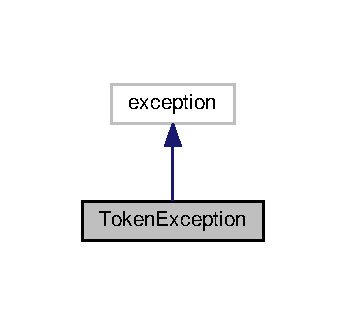
\includegraphics[width=166pt]{class_token_exception__inherit__graph}
\end{center}
\end{figure}


Collaboration diagram for Token\-Exception\-:\nopagebreak
\begin{figure}[H]
\begin{center}
\leavevmode
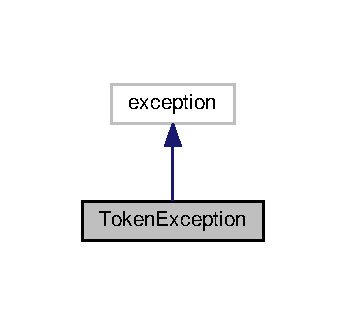
\includegraphics[width=166pt]{class_token_exception__coll__graph}
\end{center}
\end{figure}
\subsection*{Public Member Functions}
\begin{DoxyCompactItemize}
\item 
\hyperlink{class_token_exception_ace36519dfa1cf44875d33d2e3af8016b}{Token\-Exception} ()
\item 
\hyperlink{class_token_exception_a32cbe05a6ccaa1289912d570bb9b8497}{Token\-Exception} (const char $\ast$\-\_\-msg)
\item 
virtual const char $\ast$ \hyperlink{class_token_exception_a595cbd7a585aa6d1ec0c492e285b4897}{what} () const   throw ()
\end{DoxyCompactItemize}
\subsection*{Static Public Attributes}
\begin{DoxyCompactItemize}
\item 
static const int \hyperlink{class_token_exception_a0ffd72404ff477be6728f32775735554}{msg\-\_\-maxlength} = 127
\end{DoxyCompactItemize}


\subsection{Detailed Description}
exception yang dilempar kelas token 

\subsection{Constructor \& Destructor Documentation}
\hypertarget{class_token_exception_ace36519dfa1cf44875d33d2e3af8016b}{\index{Token\-Exception@{Token\-Exception}!Token\-Exception@{Token\-Exception}}
\index{Token\-Exception@{Token\-Exception}!TokenException@{Token\-Exception}}
\subsubsection[{Token\-Exception}]{\setlength{\rightskip}{0pt plus 5cm}Token\-Exception\-::\-Token\-Exception (
\begin{DoxyParamCaption}
{}
\end{DoxyParamCaption}
)\hspace{0.3cm}{\ttfamily [inline]}}}\label{class_token_exception_ace36519dfa1cf44875d33d2e3af8016b}
\hypertarget{class_token_exception_a32cbe05a6ccaa1289912d570bb9b8497}{\index{Token\-Exception@{Token\-Exception}!Token\-Exception@{Token\-Exception}}
\index{Token\-Exception@{Token\-Exception}!TokenException@{Token\-Exception}}
\subsubsection[{Token\-Exception}]{\setlength{\rightskip}{0pt plus 5cm}Token\-Exception\-::\-Token\-Exception (
\begin{DoxyParamCaption}
\item[{const char $\ast$}]{\-\_\-msg}
\end{DoxyParamCaption}
)\hspace{0.3cm}{\ttfamily [inline]}}}\label{class_token_exception_a32cbe05a6ccaa1289912d570bb9b8497}


\subsection{Member Function Documentation}
\hypertarget{class_token_exception_a595cbd7a585aa6d1ec0c492e285b4897}{\index{Token\-Exception@{Token\-Exception}!what@{what}}
\index{what@{what}!TokenException@{Token\-Exception}}
\subsubsection[{what}]{\setlength{\rightskip}{0pt plus 5cm}virtual const char$\ast$ Token\-Exception\-::what (
\begin{DoxyParamCaption}
{}
\end{DoxyParamCaption}
) const throw  ) \hspace{0.3cm}{\ttfamily [inline]}, {\ttfamily [virtual]}}}\label{class_token_exception_a595cbd7a585aa6d1ec0c492e285b4897}


\subsection{Member Data Documentation}
\hypertarget{class_token_exception_a0ffd72404ff477be6728f32775735554}{\index{Token\-Exception@{Token\-Exception}!msg\-\_\-maxlength@{msg\-\_\-maxlength}}
\index{msg\-\_\-maxlength@{msg\-\_\-maxlength}!TokenException@{Token\-Exception}}
\subsubsection[{msg\-\_\-maxlength}]{\setlength{\rightskip}{0pt plus 5cm}const int Token\-Exception\-::msg\-\_\-maxlength = 127\hspace{0.3cm}{\ttfamily [static]}}}\label{class_token_exception_a0ffd72404ff477be6728f32775735554}


The documentation for this class was generated from the following files\-:\begin{DoxyCompactItemize}
\item 
/home/nim\-\_\-13512501/\-Documents/tubes 1 O\-O\-P/src/token/\hyperlink{_token_8h}{Token.\-h}\item 
/home/nim\-\_\-13512501/\-Documents/tubes 1 O\-O\-P/src/token/\hyperlink{_token_8cpp}{Token.\-cpp}\end{DoxyCompactItemize}

\hypertarget{class_u_i}{\section{U\-I Class Reference}
\label{class_u_i}\index{U\-I@{U\-I}}
}


{\ttfamily \#include $<$U\-I.\-h$>$}

\subsection*{Public Member Functions}
\begin{DoxyCompactItemize}
\item 
\hyperlink{class_u_i_a9a3a698a1e40dd0de36466b103b3e0ba}{U\-I} (std\-::istream \&\-\_\-in=std\-::cin, std\-::ostream \&\-\_\-out=std\-::cout)
\item 
std\-::string \hyperlink{class_u_i_a75865c47733611706c39305240774497}{Get\-Next\-Cmd} ()
\begin{DoxyCompactList}\small\item\em mendapatkan perintah. \end{DoxyCompactList}\item 
void \hyperlink{class_u_i_a0f9ea0a04b6425c6aee3d01f269676e9}{Display} (std\-::string dsp)
\begin{DoxyCompactList}\small\item\em menampilkan respon \end{DoxyCompactList}\end{DoxyCompactItemize}


\subsection{Constructor \& Destructor Documentation}
\hypertarget{class_u_i_a9a3a698a1e40dd0de36466b103b3e0ba}{\index{U\-I@{U\-I}!U\-I@{U\-I}}
\index{U\-I@{U\-I}!UI@{U\-I}}
\subsubsection[{U\-I}]{\setlength{\rightskip}{0pt plus 5cm}U\-I\-::\-U\-I (
\begin{DoxyParamCaption}
\item[{std\-::istream \&}]{\-\_\-in = {\ttfamily std\-:\-:cin}, }
\item[{std\-::ostream \&}]{\-\_\-out = {\ttfamily std\-:\-:cout}}
\end{DoxyParamCaption}
)\hspace{0.3cm}{\ttfamily [inline]}}}\label{class_u_i_a9a3a698a1e40dd0de36466b103b3e0ba}


\subsection{Member Function Documentation}
\hypertarget{class_u_i_a0f9ea0a04b6425c6aee3d01f269676e9}{\index{U\-I@{U\-I}!Display@{Display}}
\index{Display@{Display}!UI@{U\-I}}
\subsubsection[{Display}]{\setlength{\rightskip}{0pt plus 5cm}void U\-I\-::\-Display (
\begin{DoxyParamCaption}
\item[{std\-::string}]{dsp}
\end{DoxyParamCaption}
)\hspace{0.3cm}{\ttfamily [inline]}}}\label{class_u_i_a0f9ea0a04b6425c6aee3d01f269676e9}


menampilkan respon 

\hypertarget{class_u_i_a75865c47733611706c39305240774497}{\index{U\-I@{U\-I}!Get\-Next\-Cmd@{Get\-Next\-Cmd}}
\index{Get\-Next\-Cmd@{Get\-Next\-Cmd}!UI@{U\-I}}
\subsubsection[{Get\-Next\-Cmd}]{\setlength{\rightskip}{0pt plus 5cm}std\-::string U\-I\-::\-Get\-Next\-Cmd (
\begin{DoxyParamCaption}
{}
\end{DoxyParamCaption}
)\hspace{0.3cm}{\ttfamily [inline]}}}\label{class_u_i_a75865c47733611706c39305240774497}


mendapatkan perintah. 



The documentation for this class was generated from the following file\-:\begin{DoxyCompactItemize}
\item 
/home/nim\-\_\-13512501/\-Documents/tubes 1 O\-O\-P/src/\hyperlink{_u_i_8h}{U\-I.\-h}\end{DoxyCompactItemize}

\chapter{File Documentation}
\hypertarget{_evaluator_8cpp}{\section{/home/nim\-\_\-13512501/\-Documents/tubes 1 O\-O\-P/src/\-Evaluator.cpp File Reference}
\label{_evaluator_8cpp}\index{/home/nim\-\_\-13512501/\-Documents/tubes 1 O\-O\-P/src/\-Evaluator.\-cpp@{/home/nim\-\_\-13512501/\-Documents/tubes 1 O\-O\-P/src/\-Evaluator.\-cpp}}
}
{\ttfamily \#include \char`\"{}Evaluator.\-h\char`\"{}}\\*
{\ttfamily \#include \char`\"{}stack/stack.\-h\char`\"{}}\\*
{\ttfamily \#include \char`\"{}token/mesintoken.\-h\char`\"{}}\\*
{\ttfamily \#include \char`\"{}File\-Manager.\-h\char`\"{}}\\*
{\ttfamily \#include $<$cassert$>$}\\*
{\ttfamily \#include $<$sstream$>$}\\*
{\ttfamily \#include $<$cstdlib$>$}\\*
{\ttfamily \#include $<$cstring$>$}\\*
Include dependency graph for Evaluator.\-cpp\-:\nopagebreak
\begin{figure}[H]
\begin{center}
\leavevmode
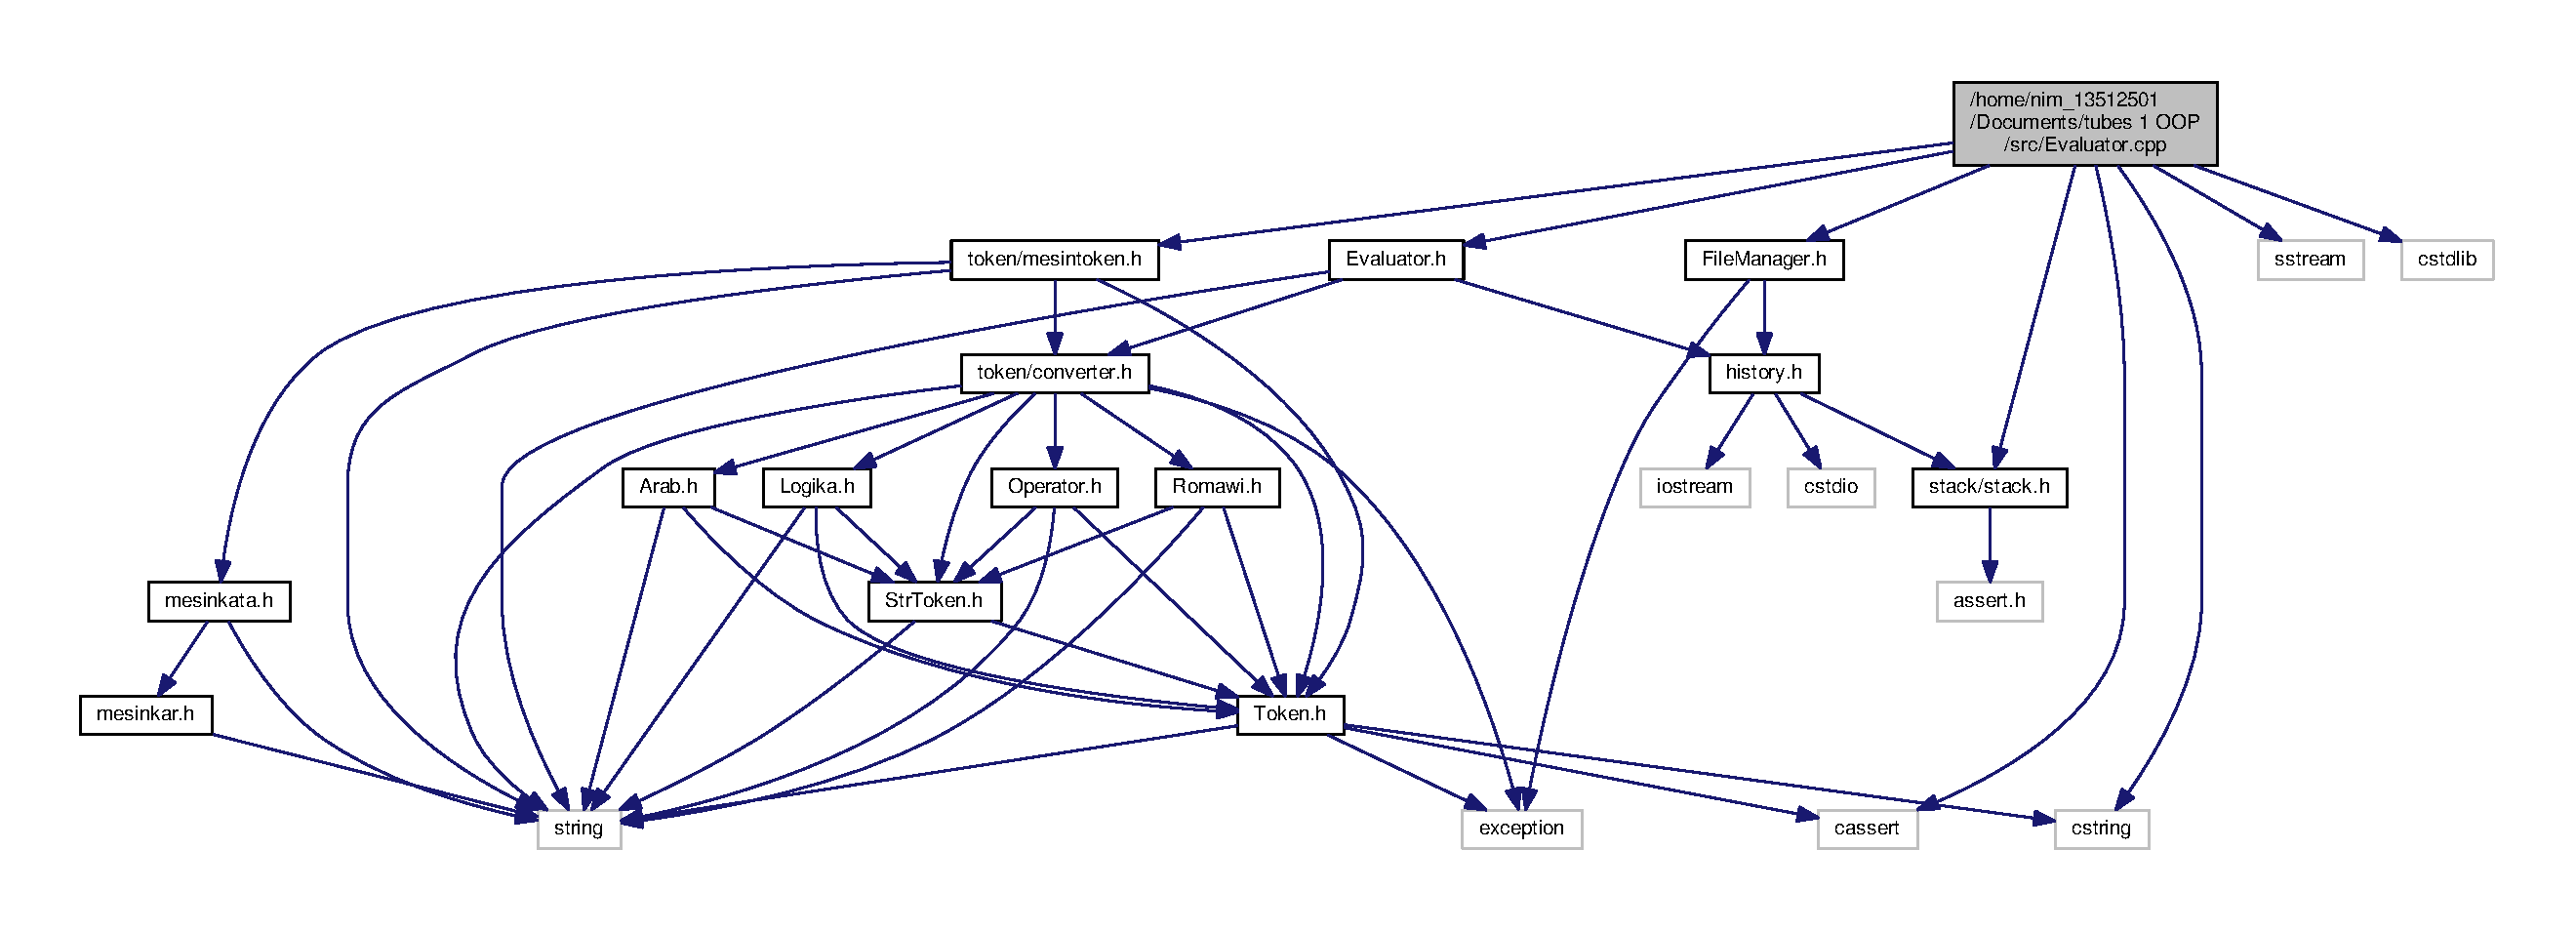
\includegraphics[width=350pt]{_evaluator_8cpp__incl}
\end{center}
\end{figure}

\hypertarget{_evaluator_8h}{\section{/home/nim\-\_\-13512501/\-Documents/tubes 1 O\-O\-P/src/\-Evaluator.h File Reference}
\label{_evaluator_8h}\index{/home/nim\-\_\-13512501/\-Documents/tubes 1 O\-O\-P/src/\-Evaluator.\-h@{/home/nim\-\_\-13512501/\-Documents/tubes 1 O\-O\-P/src/\-Evaluator.\-h}}
}
{\ttfamily \#include \char`\"{}token/converter.\-h\char`\"{}}\\*
{\ttfamily \#include $<$string$>$}\\*
{\ttfamily \#include \char`\"{}history.\-h\char`\"{}}\\*
Include dependency graph for Evaluator.\-h\-:\nopagebreak
\begin{figure}[H]
\begin{center}
\leavevmode
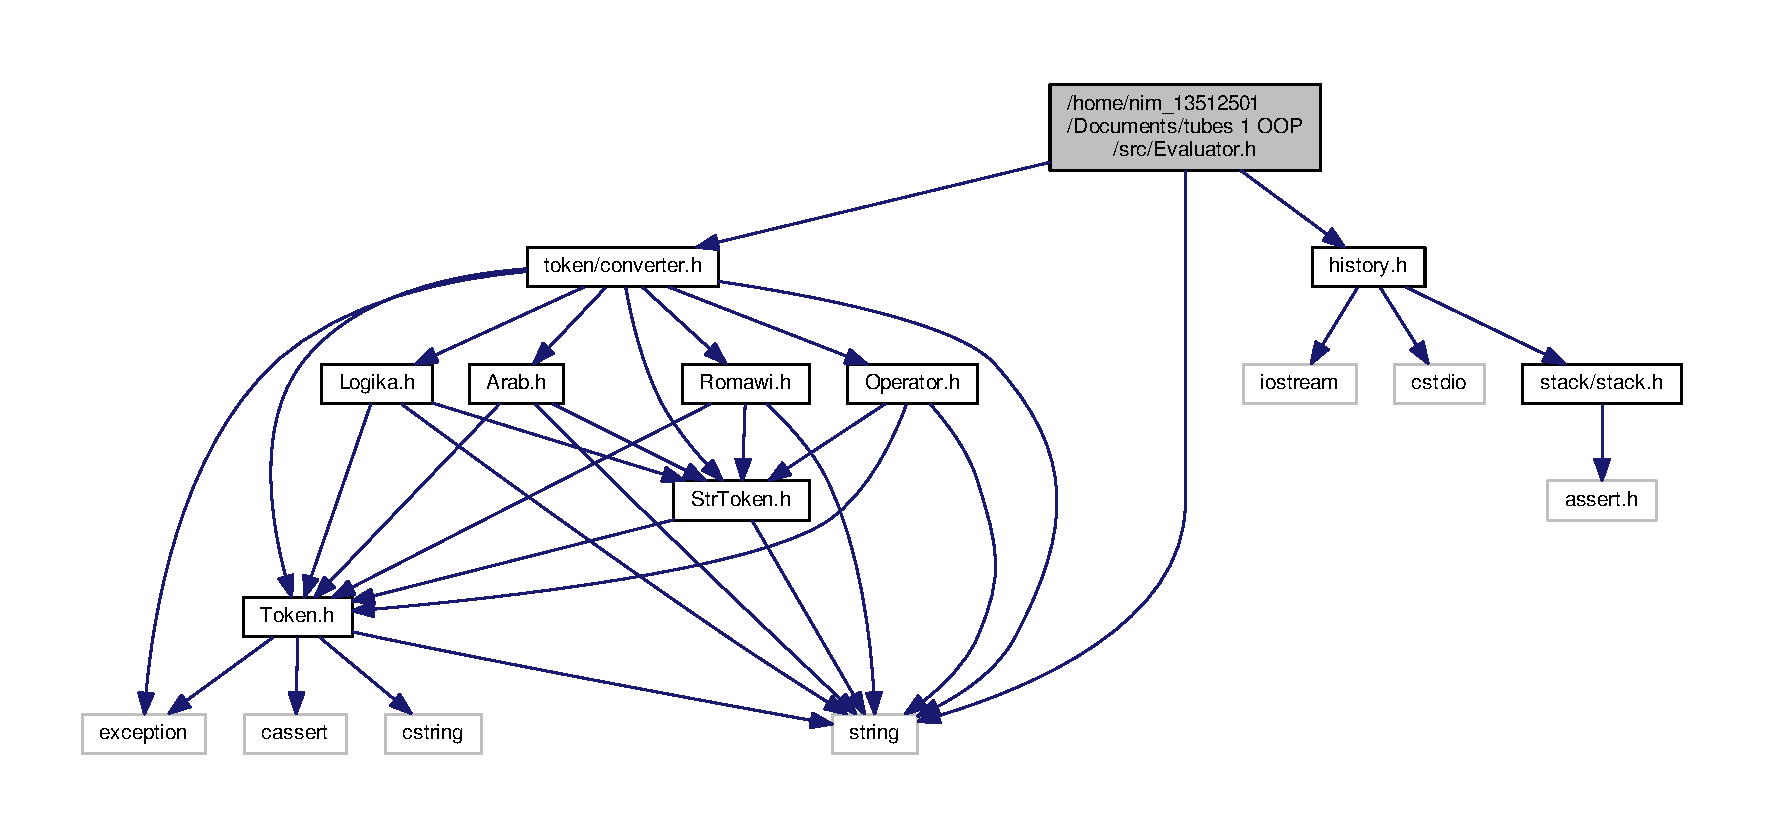
\includegraphics[width=350pt]{_evaluator_8h__incl}
\end{center}
\end{figure}
This graph shows which files directly or indirectly include this file\-:\nopagebreak
\begin{figure}[H]
\begin{center}
\leavevmode
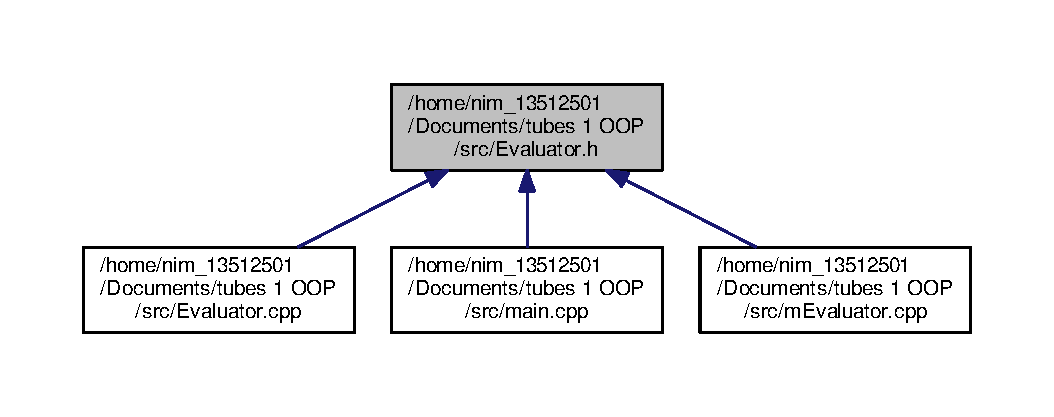
\includegraphics[width=350pt]{_evaluator_8h__dep__incl}
\end{center}
\end{figure}
\subsection*{Classes}
\begin{DoxyCompactItemize}
\item 
class \hyperlink{class_evaluator}{Evaluator}
\end{DoxyCompactItemize}

\hypertarget{_file_manager_8cpp}{\section{/home/nim\-\_\-13512501/\-Documents/tubes 1 O\-O\-P/src/\-File\-Manager.cpp File Reference}
\label{_file_manager_8cpp}\index{/home/nim\-\_\-13512501/\-Documents/tubes 1 O\-O\-P/src/\-File\-Manager.\-cpp@{/home/nim\-\_\-13512501/\-Documents/tubes 1 O\-O\-P/src/\-File\-Manager.\-cpp}}
}
{\ttfamily \#include \char`\"{}File\-Manager.\-h\char`\"{}}\\*
{\ttfamily \#include $<$fstream$>$}\\*
{\ttfamily \#include $<$ctime$>$}\\*
Include dependency graph for File\-Manager.\-cpp\-:\nopagebreak
\begin{figure}[H]
\begin{center}
\leavevmode
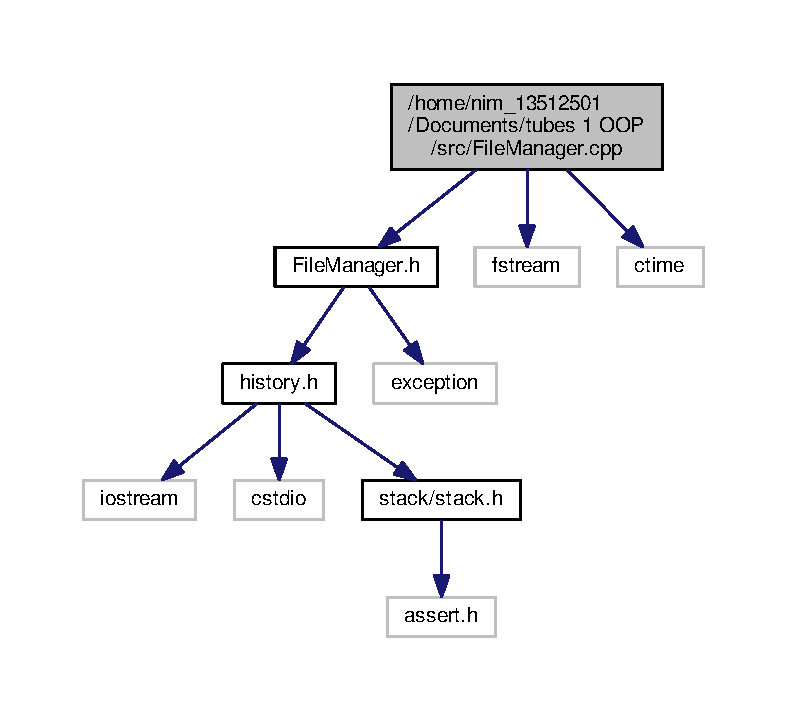
\includegraphics[width=350pt]{_file_manager_8cpp__incl}
\end{center}
\end{figure}

\hypertarget{_file_manager_8h}{\section{/home/nim\-\_\-13512501/\-Documents/tubes 1 O\-O\-P/src/\-File\-Manager.h File Reference}
\label{_file_manager_8h}\index{/home/nim\-\_\-13512501/\-Documents/tubes 1 O\-O\-P/src/\-File\-Manager.\-h@{/home/nim\-\_\-13512501/\-Documents/tubes 1 O\-O\-P/src/\-File\-Manager.\-h}}
}
{\ttfamily \#include \char`\"{}history.\-h\char`\"{}}\\*
{\ttfamily \#include $<$exception$>$}\\*
Include dependency graph for File\-Manager.\-h\-:\nopagebreak
\begin{figure}[H]
\begin{center}
\leavevmode
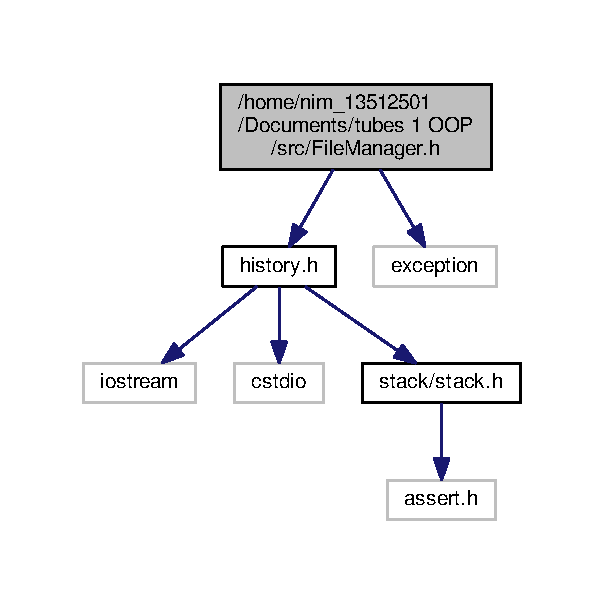
\includegraphics[width=290pt]{_file_manager_8h__incl}
\end{center}
\end{figure}
This graph shows which files directly or indirectly include this file\-:\nopagebreak
\begin{figure}[H]
\begin{center}
\leavevmode
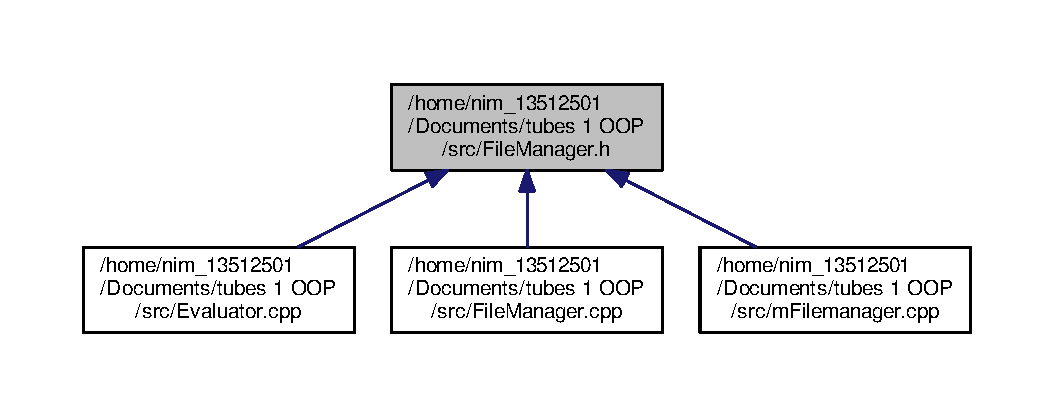
\includegraphics[width=350pt]{_file_manager_8h__dep__incl}
\end{center}
\end{figure}
\subsection*{Classes}
\begin{DoxyCompactItemize}
\item 
class \hyperlink{class_file_manager}{File\-Manager}
\item 
class \hyperlink{class_file_manager_exception}{File\-Manager\-Exception}
\begin{DoxyCompactList}\small\item\em exception yang dilempar oleh \hyperlink{class_file_manager}{File\-Manager} \end{DoxyCompactList}\end{DoxyCompactItemize}

\hypertarget{history_8cpp}{\section{/home/nim\-\_\-13512501/\-Documents/tubes 1 O\-O\-P/src/history.cpp File Reference}
\label{history_8cpp}\index{/home/nim\-\_\-13512501/\-Documents/tubes 1 O\-O\-P/src/history.\-cpp@{/home/nim\-\_\-13512501/\-Documents/tubes 1 O\-O\-P/src/history.\-cpp}}
}
{\ttfamily \#include $<$iostream$>$}\\*
{\ttfamily \#include $<$cstdio$>$}\\*
{\ttfamily \#include \char`\"{}history.\-h\char`\"{}}\\*
Include dependency graph for history.\-cpp\-:\nopagebreak
\begin{figure}[H]
\begin{center}
\leavevmode
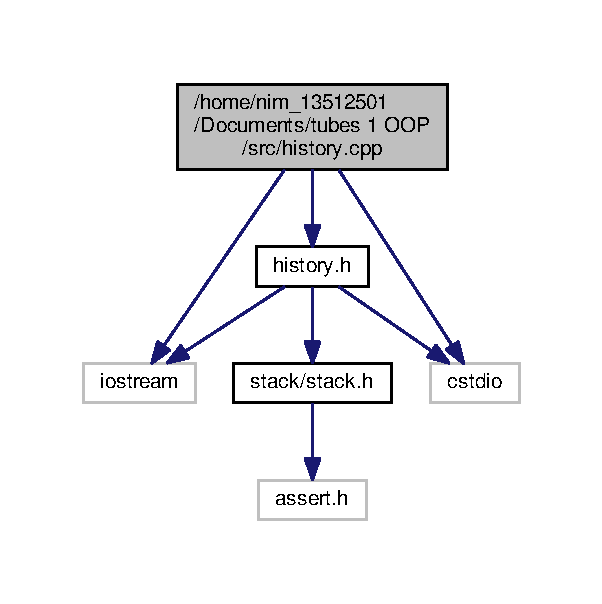
\includegraphics[width=289pt]{history_8cpp__incl}
\end{center}
\end{figure}

\hypertarget{history_8h}{\section{/home/nim\-\_\-13512501/\-Documents/tubes 1 O\-O\-P/src/history.h File Reference}
\label{history_8h}\index{/home/nim\-\_\-13512501/\-Documents/tubes 1 O\-O\-P/src/history.\-h@{/home/nim\-\_\-13512501/\-Documents/tubes 1 O\-O\-P/src/history.\-h}}
}
{\ttfamily \#include $<$iostream$>$}\\*
{\ttfamily \#include $<$cstdio$>$}\\*
{\ttfamily \#include \char`\"{}stack/stack.\-h\char`\"{}}\\*
Include dependency graph for history.\-h\-:\nopagebreak
\begin{figure}[H]
\begin{center}
\leavevmode
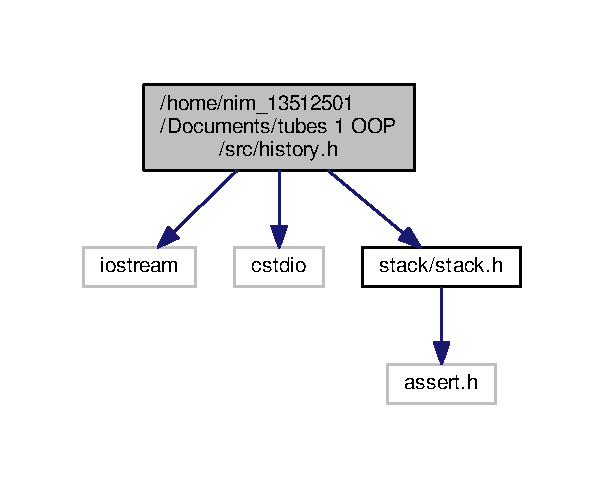
\includegraphics[width=290pt]{history_8h__incl}
\end{center}
\end{figure}
This graph shows which files directly or indirectly include this file\-:\nopagebreak
\begin{figure}[H]
\begin{center}
\leavevmode
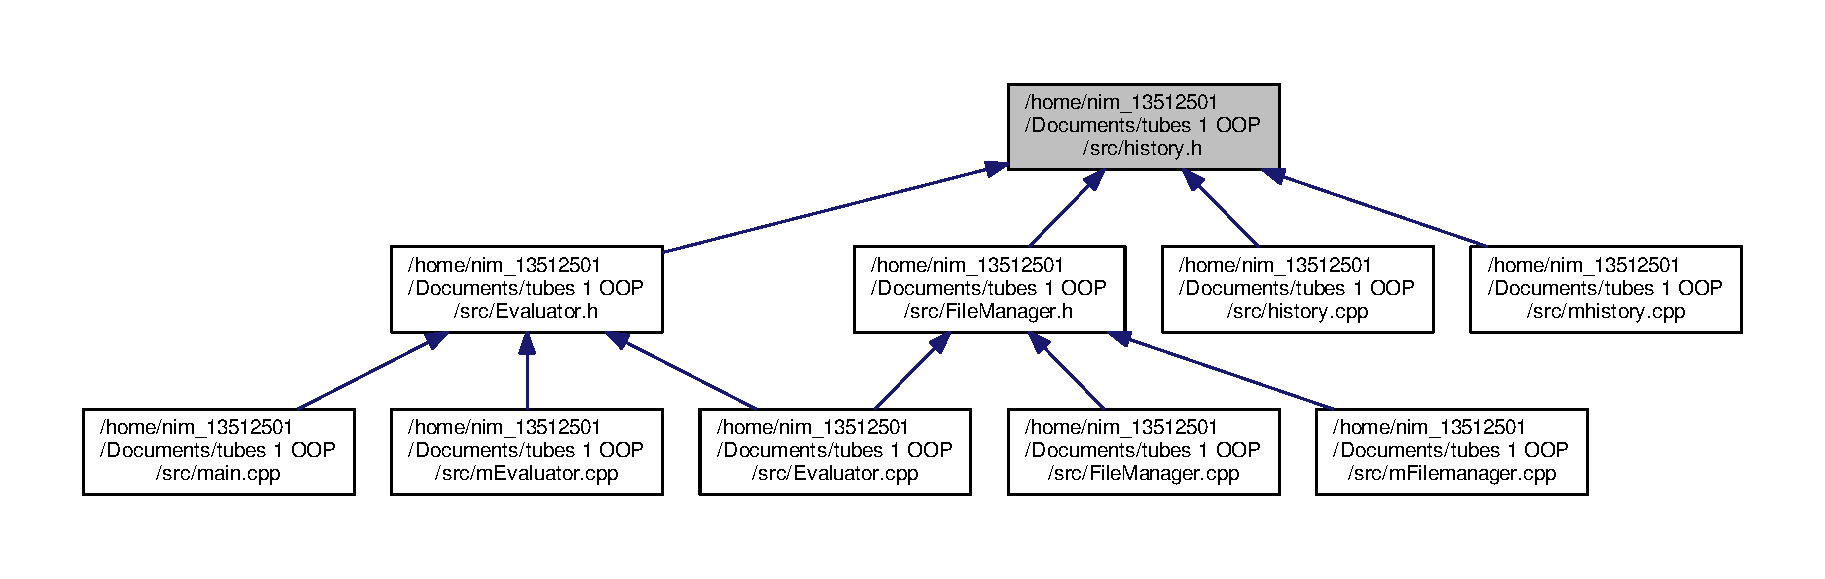
\includegraphics[width=350pt]{history_8h__dep__incl}
\end{center}
\end{figure}
\subsection*{Classes}
\begin{DoxyCompactItemize}
\item 
class \hyperlink{class_history}{History}
\end{DoxyCompactItemize}

\hypertarget{mainkar_8cpp}{\section{/home/nim\-\_\-13512501/\-Documents/tubes 1 O\-O\-P/src/katakr/mainkar.cpp File Reference}
\label{mainkar_8cpp}\index{/home/nim\-\_\-13512501/\-Documents/tubes 1 O\-O\-P/src/katakr/mainkar.\-cpp@{/home/nim\-\_\-13512501/\-Documents/tubes 1 O\-O\-P/src/katakr/mainkar.\-cpp}}
}
{\ttfamily \#include \char`\"{}mesinkar.\-h\char`\"{}}\\*
{\ttfamily \#include $<$iostream$>$}\\*
{\ttfamily \#include $<$cassert$>$}\\*
Include dependency graph for mainkar.\-cpp\-:\nopagebreak
\begin{figure}[H]
\begin{center}
\leavevmode
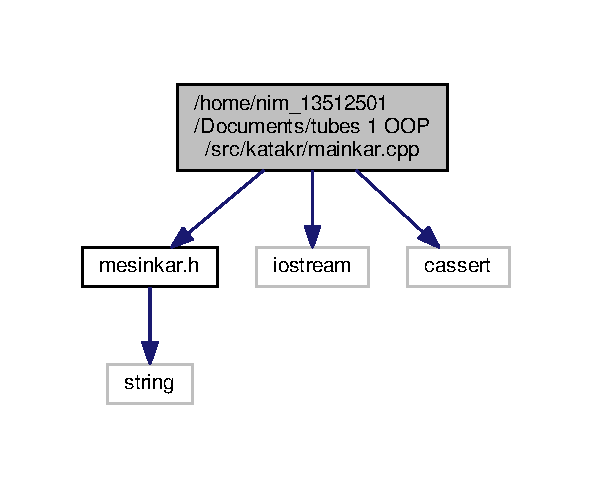
\includegraphics[width=284pt]{mainkar_8cpp__incl}
\end{center}
\end{figure}
\subsection*{Functions}
\begin{DoxyCompactItemize}
\item 
int \hyperlink{mainkar_8cpp_ae66f6b31b5ad750f1fe042a706a4e3d4}{main} ()
\end{DoxyCompactItemize}


\subsection{Function Documentation}
\hypertarget{mainkar_8cpp_ae66f6b31b5ad750f1fe042a706a4e3d4}{\index{mainkar.\-cpp@{mainkar.\-cpp}!main@{main}}
\index{main@{main}!mainkar.cpp@{mainkar.\-cpp}}
\subsubsection[{main}]{\setlength{\rightskip}{0pt plus 5cm}int main (
\begin{DoxyParamCaption}
{}
\end{DoxyParamCaption}
)}}\label{mainkar_8cpp_ae66f6b31b5ad750f1fe042a706a4e3d4}
Driver untuk mengetes kelas mesinkarakter 
\hypertarget{mainkata_8cpp}{\section{/home/nim\-\_\-13512501/\-Documents/tubes 1 O\-O\-P/src/katakr/mainkata.cpp File Reference}
\label{mainkata_8cpp}\index{/home/nim\-\_\-13512501/\-Documents/tubes 1 O\-O\-P/src/katakr/mainkata.\-cpp@{/home/nim\-\_\-13512501/\-Documents/tubes 1 O\-O\-P/src/katakr/mainkata.\-cpp}}
}
{\ttfamily \#include $<$cassert$>$}\\*
{\ttfamily \#include $<$iostream$>$}\\*
{\ttfamily \#include \char`\"{}mesinkata.\-h\char`\"{}}\\*
Include dependency graph for mainkata.\-cpp\-:\nopagebreak
\begin{figure}[H]
\begin{center}
\leavevmode
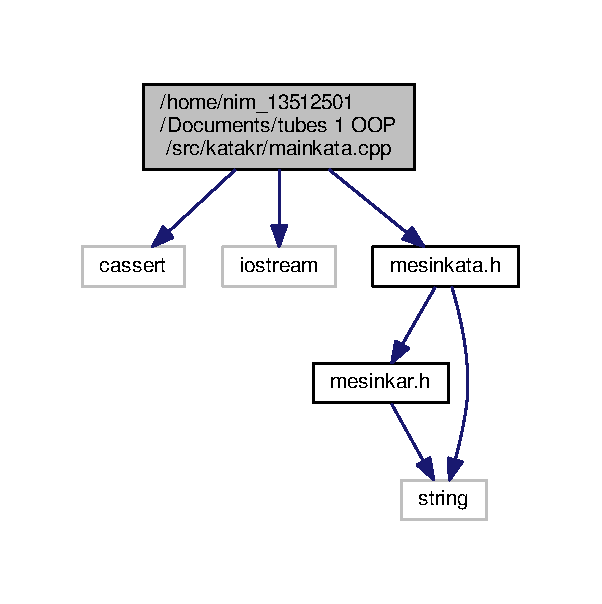
\includegraphics[width=289pt]{mainkata_8cpp__incl}
\end{center}
\end{figure}
\subsection*{Functions}
\begin{DoxyCompactItemize}
\item 
int \hyperlink{mainkata_8cpp_ae66f6b31b5ad750f1fe042a706a4e3d4}{main} ()
\end{DoxyCompactItemize}


\subsection{Function Documentation}
\hypertarget{mainkata_8cpp_ae66f6b31b5ad750f1fe042a706a4e3d4}{\index{mainkata.\-cpp@{mainkata.\-cpp}!main@{main}}
\index{main@{main}!mainkata.cpp@{mainkata.\-cpp}}
\subsubsection[{main}]{\setlength{\rightskip}{0pt plus 5cm}int main (
\begin{DoxyParamCaption}
{}
\end{DoxyParamCaption}
)}}\label{mainkata_8cpp_ae66f6b31b5ad750f1fe042a706a4e3d4}

\hypertarget{mesinkar_8cpp}{\section{/home/nim\-\_\-13512501/\-Documents/tubes 1 O\-O\-P/src/katakr/mesinkar.cpp File Reference}
\label{mesinkar_8cpp}\index{/home/nim\-\_\-13512501/\-Documents/tubes 1 O\-O\-P/src/katakr/mesinkar.\-cpp@{/home/nim\-\_\-13512501/\-Documents/tubes 1 O\-O\-P/src/katakr/mesinkar.\-cpp}}
}
{\ttfamily \#include \char`\"{}mesinkar.\-h\char`\"{}}\\*
{\ttfamily \#include $<$string$>$}\\*
{\ttfamily \#include $<$assert.\-h$>$}\\*
Include dependency graph for mesinkar.\-cpp\-:\nopagebreak
\begin{figure}[H]
\begin{center}
\leavevmode
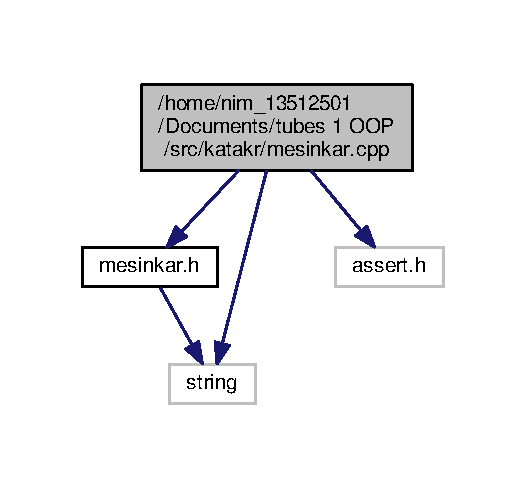
\includegraphics[width=253pt]{mesinkar_8cpp__incl}
\end{center}
\end{figure}

\hypertarget{katakr_2mesinkar_8h}{\section{/home/nim\-\_\-13512501/\-Documents/tubes 1 O\-O\-P/src/katakr/mesinkar.h File Reference}
\label{katakr_2mesinkar_8h}\index{/home/nim\-\_\-13512501/\-Documents/tubes 1 O\-O\-P/src/katakr/mesinkar.\-h@{/home/nim\-\_\-13512501/\-Documents/tubes 1 O\-O\-P/src/katakr/mesinkar.\-h}}
}
{\ttfamily \#include $<$string$>$}\\*
Include dependency graph for mesinkar.\-h\-:\nopagebreak
\begin{figure}[H]
\begin{center}
\leavevmode
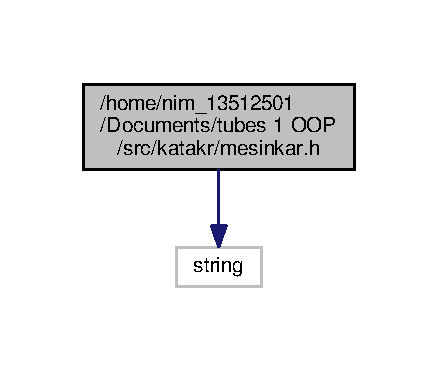
\includegraphics[width=210pt]{katakr_2mesinkar_8h__incl}
\end{center}
\end{figure}
This graph shows which files directly or indirectly include this file\-:\nopagebreak
\begin{figure}[H]
\begin{center}
\leavevmode
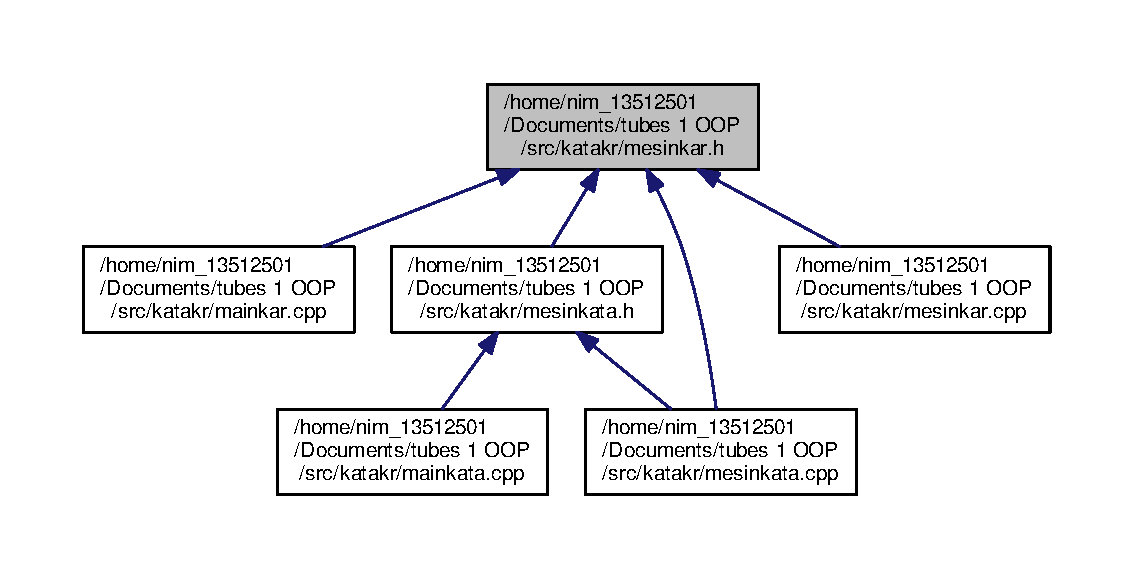
\includegraphics[width=350pt]{katakr_2mesinkar_8h__dep__incl}
\end{center}
\end{figure}
\subsection*{Classes}
\begin{DoxyCompactItemize}
\item 
class \hyperlink{classmesinkar}{mesinkar}
\end{DoxyCompactItemize}

\hypertarget{token_2mesinkar_8h}{\section{/home/nim\-\_\-13512501/\-Documents/tubes 1 O\-O\-P/src/token/mesinkar.h File Reference}
\label{token_2mesinkar_8h}\index{/home/nim\-\_\-13512501/\-Documents/tubes 1 O\-O\-P/src/token/mesinkar.\-h@{/home/nim\-\_\-13512501/\-Documents/tubes 1 O\-O\-P/src/token/mesinkar.\-h}}
}
{\ttfamily \#include $<$string$>$}\\*
Include dependency graph for mesinkar.\-h\-:\nopagebreak
\begin{figure}[H]
\begin{center}
\leavevmode
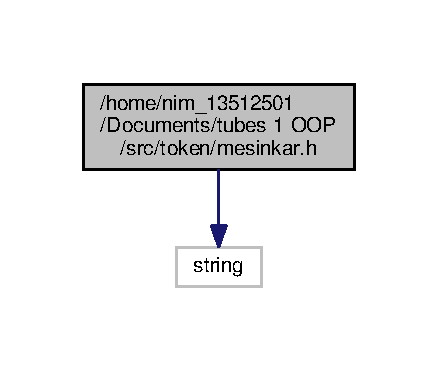
\includegraphics[width=210pt]{token_2mesinkar_8h__incl}
\end{center}
\end{figure}
This graph shows which files directly or indirectly include this file\-:\nopagebreak
\begin{figure}[H]
\begin{center}
\leavevmode
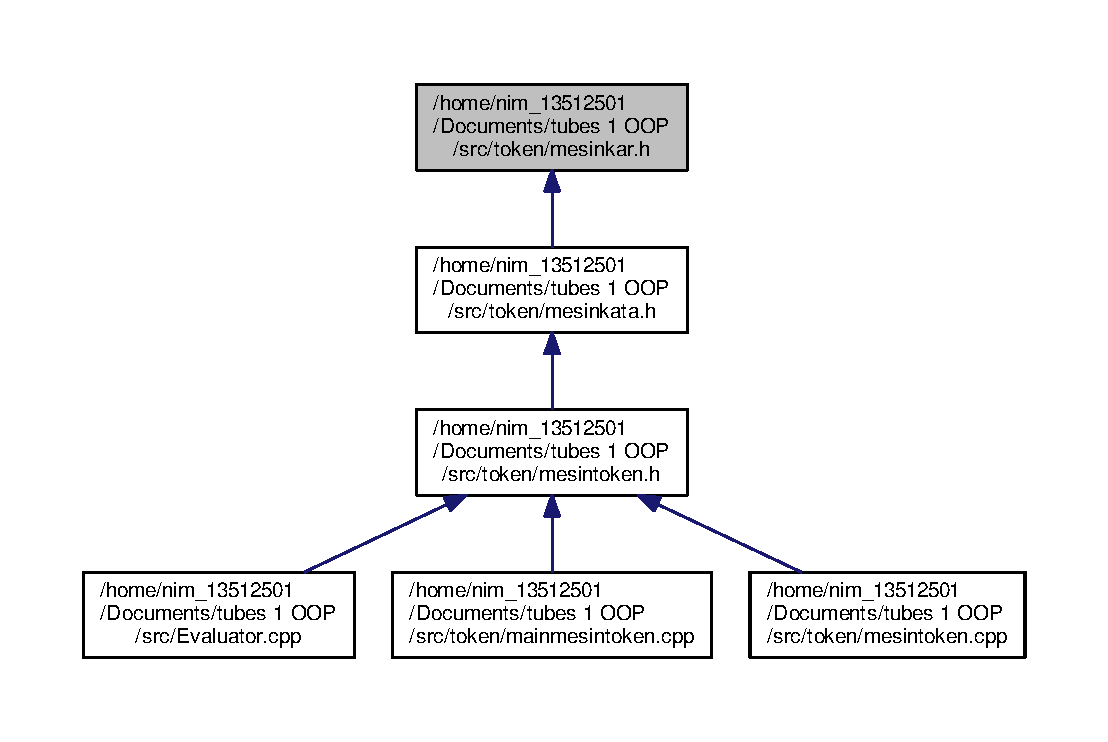
\includegraphics[width=350pt]{token_2mesinkar_8h__dep__incl}
\end{center}
\end{figure}
\subsection*{Classes}
\begin{DoxyCompactItemize}
\item 
class \hyperlink{classmesinkar}{mesinkar}
\end{DoxyCompactItemize}

\hypertarget{mesinkata_8cpp}{\section{/home/nim\-\_\-13512501/\-Documents/tubes 1 O\-O\-P/src/katakr/mesinkata.cpp File Reference}
\label{mesinkata_8cpp}\index{/home/nim\-\_\-13512501/\-Documents/tubes 1 O\-O\-P/src/katakr/mesinkata.\-cpp@{/home/nim\-\_\-13512501/\-Documents/tubes 1 O\-O\-P/src/katakr/mesinkata.\-cpp}}
}
{\ttfamily \#include \char`\"{}mesinkata.\-h\char`\"{}}\\*
{\ttfamily \#include \char`\"{}mesinkar.\-h\char`\"{}}\\*
{\ttfamily \#include $<$string$>$}\\*
{\ttfamily \#include $<$cassert$>$}\\*
Include dependency graph for mesinkata.\-cpp\-:\nopagebreak
\begin{figure}[H]
\begin{center}
\leavevmode
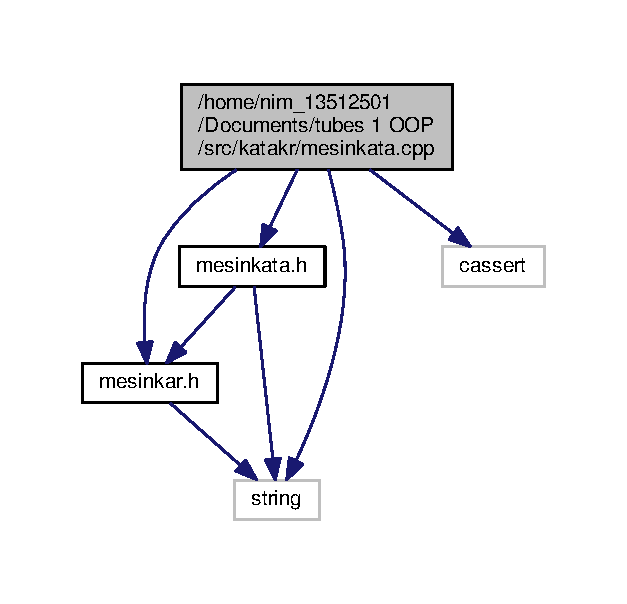
\includegraphics[width=301pt]{mesinkata_8cpp__incl}
\end{center}
\end{figure}
\subsection*{Macros}
\begin{DoxyCompactItemize}
\item 
\#define \hyperlink{mesinkata_8cpp_a5aebfba92373e0dc8a76d272bcd8e85d}{B\-L\-A\-N\-K}~' '
\end{DoxyCompactItemize}
\subsection*{Variables}
\begin{DoxyCompactItemize}
\item 
const int \hyperlink{mesinkata_8cpp_af7dbda7167e22cb3417c16f78061ad80}{M\-A\-X} =10
\end{DoxyCompactItemize}


\subsection{Macro Definition Documentation}
\hypertarget{mesinkata_8cpp_a5aebfba92373e0dc8a76d272bcd8e85d}{\index{mesinkata.\-cpp@{mesinkata.\-cpp}!B\-L\-A\-N\-K@{B\-L\-A\-N\-K}}
\index{B\-L\-A\-N\-K@{B\-L\-A\-N\-K}!mesinkata.cpp@{mesinkata.\-cpp}}
\subsubsection[{B\-L\-A\-N\-K}]{\setlength{\rightskip}{0pt plus 5cm}\#define B\-L\-A\-N\-K~' '}}\label{mesinkata_8cpp_a5aebfba92373e0dc8a76d272bcd8e85d}


\subsection{Variable Documentation}
\hypertarget{mesinkata_8cpp_af7dbda7167e22cb3417c16f78061ad80}{\index{mesinkata.\-cpp@{mesinkata.\-cpp}!M\-A\-X@{M\-A\-X}}
\index{M\-A\-X@{M\-A\-X}!mesinkata.cpp@{mesinkata.\-cpp}}
\subsubsection[{M\-A\-X}]{\setlength{\rightskip}{0pt plus 5cm}const int M\-A\-X =10}}\label{mesinkata_8cpp_af7dbda7167e22cb3417c16f78061ad80}

\hypertarget{katakr_2mesinkata_8h}{\section{/home/nim\-\_\-13512501/\-Documents/tubes 1 O\-O\-P/src/katakr/mesinkata.h File Reference}
\label{katakr_2mesinkata_8h}\index{/home/nim\-\_\-13512501/\-Documents/tubes 1 O\-O\-P/src/katakr/mesinkata.\-h@{/home/nim\-\_\-13512501/\-Documents/tubes 1 O\-O\-P/src/katakr/mesinkata.\-h}}
}
{\ttfamily \#include \char`\"{}mesinkar.\-h\char`\"{}}\\*
{\ttfamily \#include $<$string$>$}\\*
Include dependency graph for mesinkata.\-h\-:\nopagebreak
\begin{figure}[H]
\begin{center}
\leavevmode
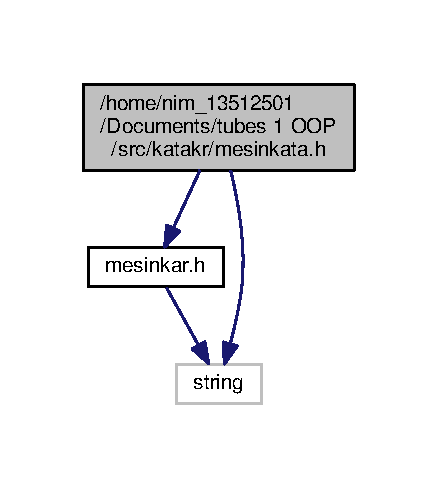
\includegraphics[width=210pt]{katakr_2mesinkata_8h__incl}
\end{center}
\end{figure}
This graph shows which files directly or indirectly include this file\-:\nopagebreak
\begin{figure}[H]
\begin{center}
\leavevmode
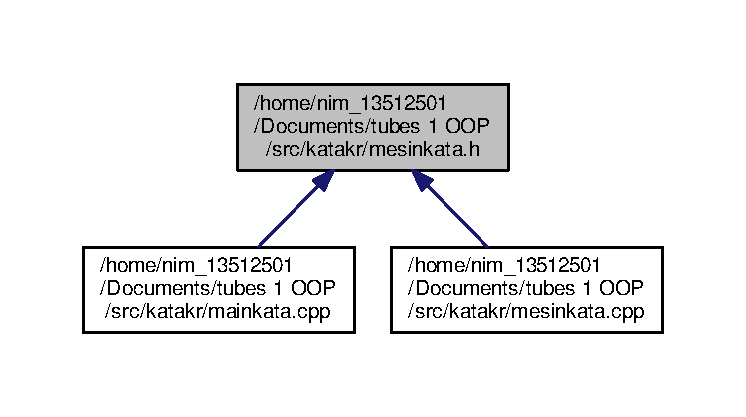
\includegraphics[width=350pt]{katakr_2mesinkata_8h__dep__incl}
\end{center}
\end{figure}
\subsection*{Classes}
\begin{DoxyCompactItemize}
\item 
class \hyperlink{classmesinkata}{mesinkata}
\begin{DoxyCompactList}\small\item\em kelas mesin kata, cara menggunakan\-: konstruksi, set pita karakter, lalu for(start();!\-End();\hyperlink{classmesinkata_aa9d334f1b013d6e2f23f791346561e76}{A\-D\-V()}) \end{DoxyCompactList}\end{DoxyCompactItemize}

\hypertarget{token_2mesinkata_8h}{\section{/home/nim\-\_\-13512501/\-Documents/tubes 1 O\-O\-P/src/token/mesinkata.h File Reference}
\label{token_2mesinkata_8h}\index{/home/nim\-\_\-13512501/\-Documents/tubes 1 O\-O\-P/src/token/mesinkata.\-h@{/home/nim\-\_\-13512501/\-Documents/tubes 1 O\-O\-P/src/token/mesinkata.\-h}}
}
{\ttfamily \#include \char`\"{}mesinkar.\-h\char`\"{}}\\*
{\ttfamily \#include $<$string$>$}\\*
Include dependency graph for mesinkata.\-h\-:\nopagebreak
\begin{figure}[H]
\begin{center}
\leavevmode
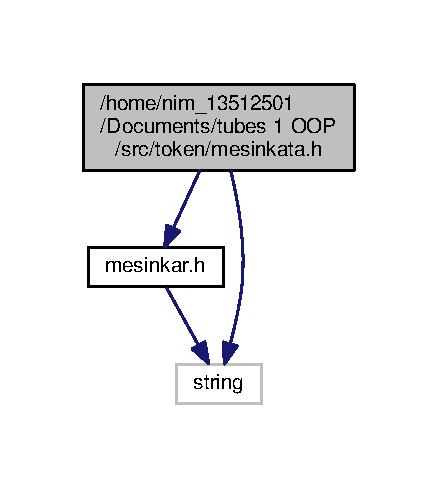
\includegraphics[width=210pt]{token_2mesinkata_8h__incl}
\end{center}
\end{figure}
This graph shows which files directly or indirectly include this file\-:\nopagebreak
\begin{figure}[H]
\begin{center}
\leavevmode
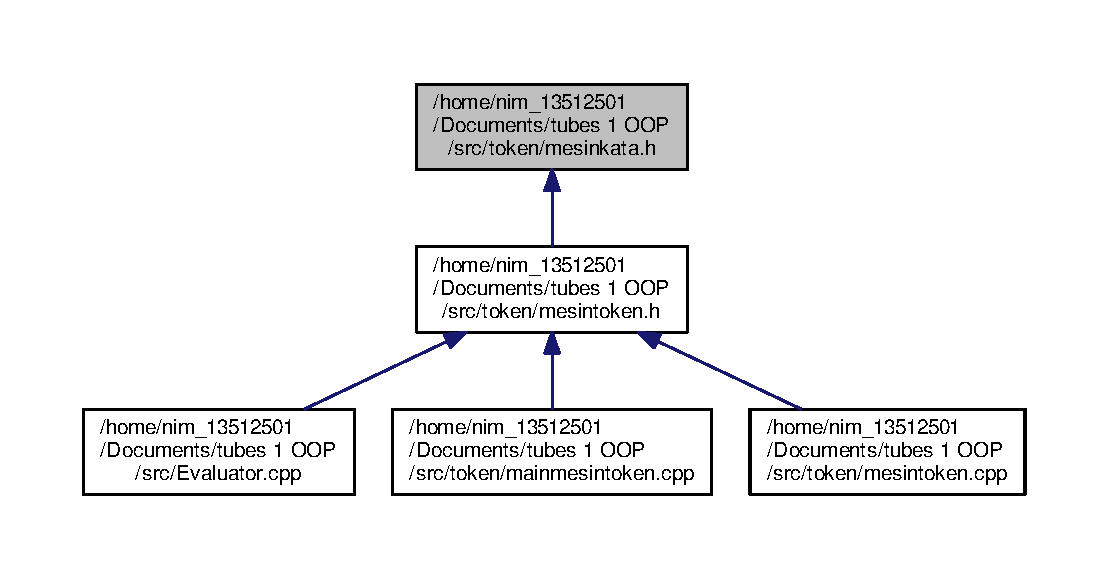
\includegraphics[width=350pt]{token_2mesinkata_8h__dep__incl}
\end{center}
\end{figure}
\subsection*{Classes}
\begin{DoxyCompactItemize}
\item 
class \hyperlink{classmesinkata}{mesinkata}
\begin{DoxyCompactList}\small\item\em kelas mesin kata, cara menggunakan\-: konstruksi, set pita karakter, lalu for(start();!\-End();\hyperlink{classmesinkata_aa9d334f1b013d6e2f23f791346561e76}{A\-D\-V()}) \end{DoxyCompactList}\end{DoxyCompactItemize}

\hypertarget{main_8cpp}{\section{/home/nim\-\_\-13512501/\-Documents/tubes 1 O\-O\-P/src/main.cpp File Reference}
\label{main_8cpp}\index{/home/nim\-\_\-13512501/\-Documents/tubes 1 O\-O\-P/src/main.\-cpp@{/home/nim\-\_\-13512501/\-Documents/tubes 1 O\-O\-P/src/main.\-cpp}}
}
{\ttfamily \#include \char`\"{}Evaluator.\-h\char`\"{}}\\*
{\ttfamily \#include \char`\"{}U\-I.\-h\char`\"{}}\\*
Include dependency graph for main.\-cpp\-:\nopagebreak
\begin{figure}[H]
\begin{center}
\leavevmode
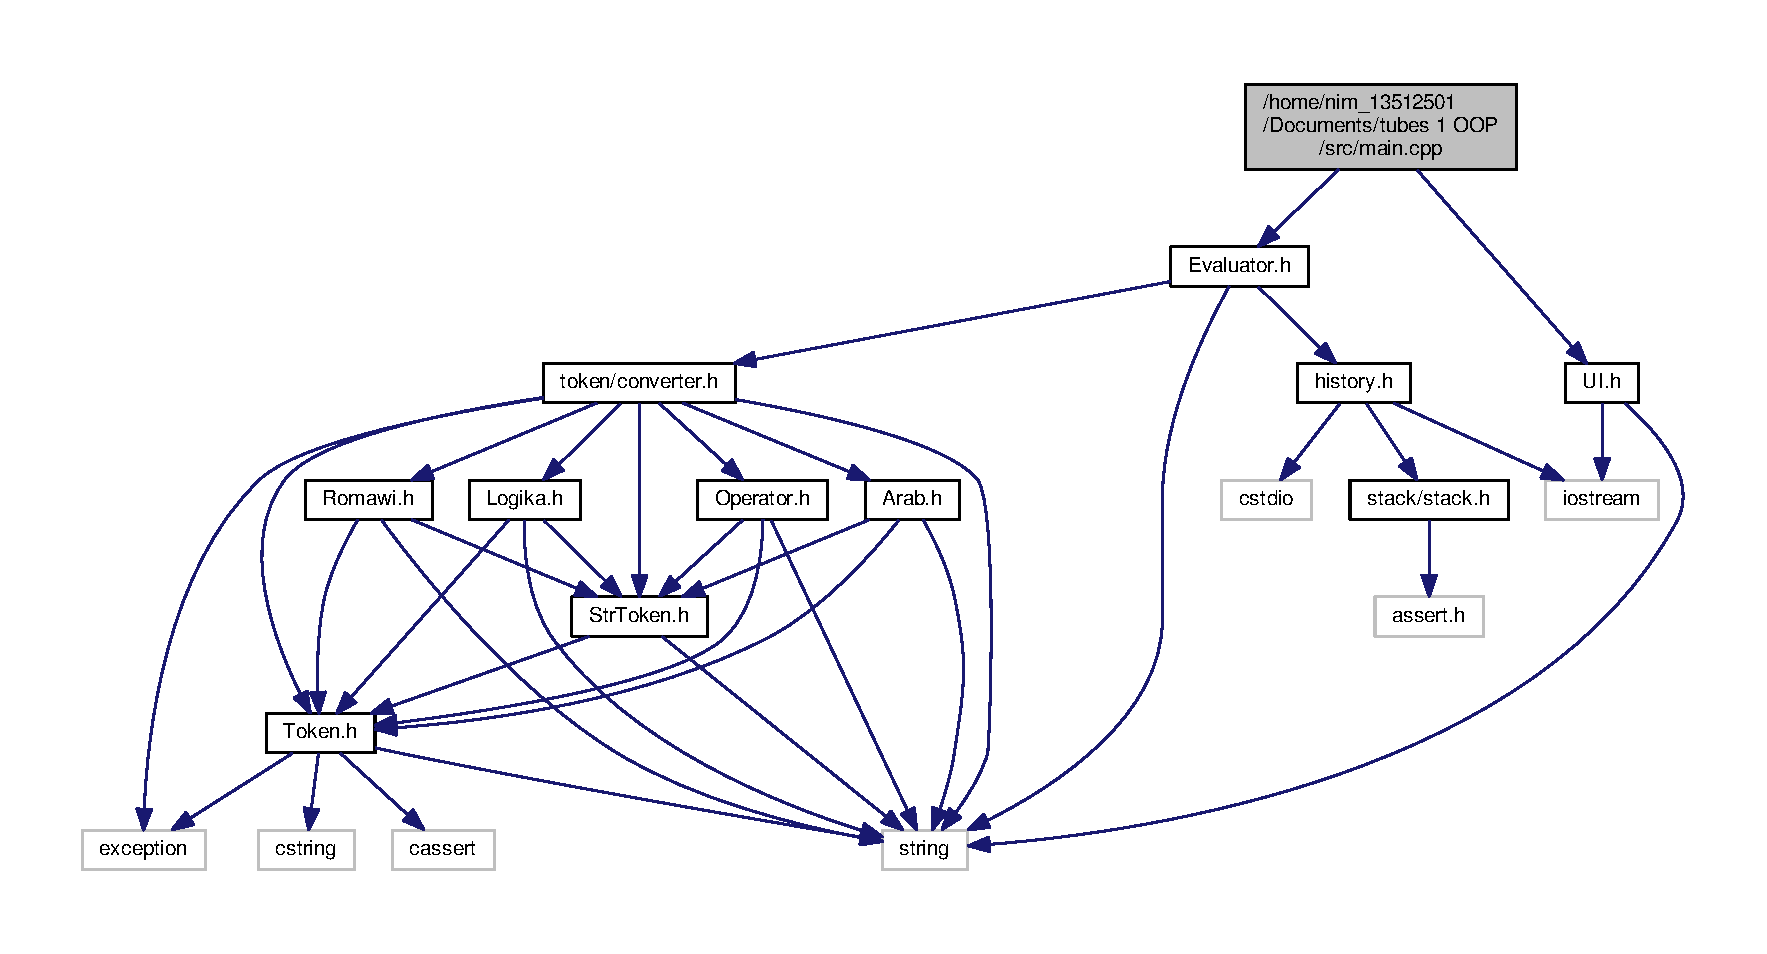
\includegraphics[width=350pt]{main_8cpp__incl}
\end{center}
\end{figure}
\subsection*{Functions}
\begin{DoxyCompactItemize}
\item 
int \hyperlink{main_8cpp_ae66f6b31b5ad750f1fe042a706a4e3d4}{main} ()
\end{DoxyCompactItemize}


\subsection{Function Documentation}
\hypertarget{main_8cpp_ae66f6b31b5ad750f1fe042a706a4e3d4}{\index{main.\-cpp@{main.\-cpp}!main@{main}}
\index{main@{main}!main.cpp@{main.\-cpp}}
\subsubsection[{main}]{\setlength{\rightskip}{0pt plus 5cm}int main (
\begin{DoxyParamCaption}
{}
\end{DoxyParamCaption}
)}}\label{main_8cpp_ae66f6b31b5ad750f1fe042a706a4e3d4}
main program ini yang di-\/compile dan di-\/link saat make memakai kelas \hyperlink{class_evaluator}{Evaluator} dan \hyperlink{class_u_i}{U\-I} 
\hypertarget{m_evaluator_8cpp}{\section{/home/nim\-\_\-13512501/\-Documents/tubes 1 O\-O\-P/src/m\-Evaluator.cpp File Reference}
\label{m_evaluator_8cpp}\index{/home/nim\-\_\-13512501/\-Documents/tubes 1 O\-O\-P/src/m\-Evaluator.\-cpp@{/home/nim\-\_\-13512501/\-Documents/tubes 1 O\-O\-P/src/m\-Evaluator.\-cpp}}
}
{\ttfamily \#include \char`\"{}Evaluator.\-h\char`\"{}}\\*
{\ttfamily \#include $<$iostream$>$}\\*
{\ttfamily \#include $<$string$>$}\\*
Include dependency graph for m\-Evaluator.\-cpp\-:\nopagebreak
\begin{figure}[H]
\begin{center}
\leavevmode
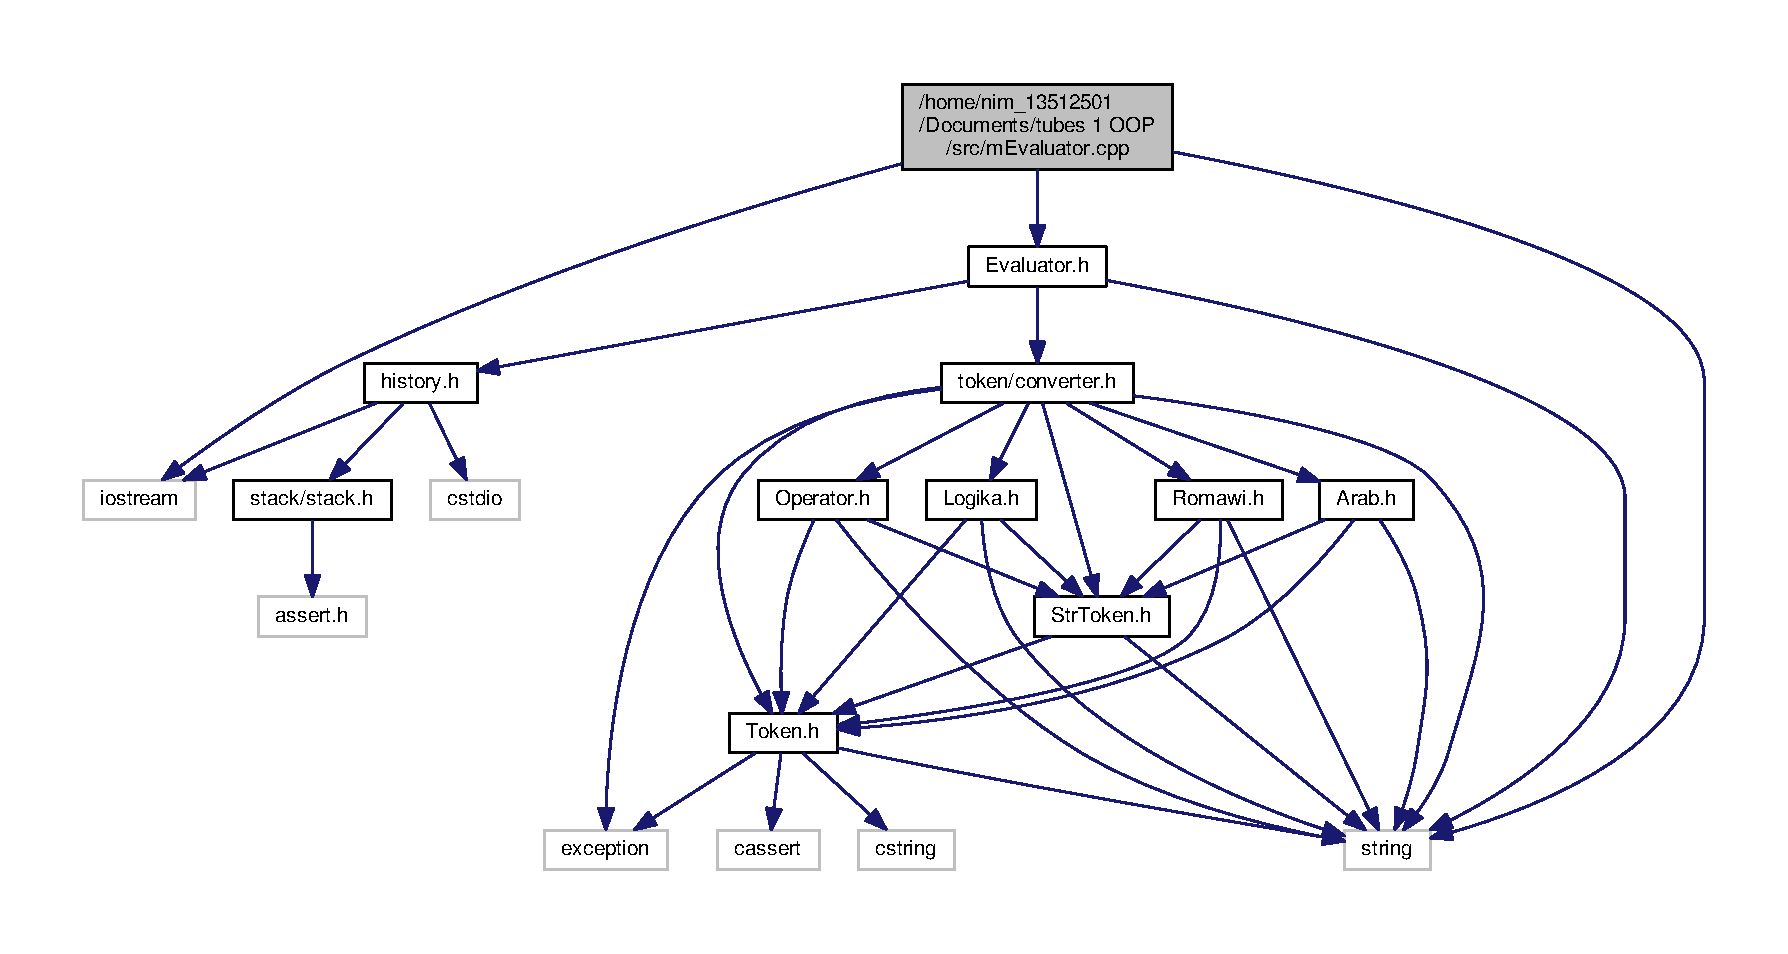
\includegraphics[width=350pt]{m_evaluator_8cpp__incl}
\end{center}
\end{figure}
\subsection*{Functions}
\begin{DoxyCompactItemize}
\item 
int \hyperlink{m_evaluator_8cpp_ae66f6b31b5ad750f1fe042a706a4e3d4}{main} ()
\begin{DoxyCompactList}\small\item\em tes kelas main \end{DoxyCompactList}\end{DoxyCompactItemize}


\subsection{Function Documentation}
\hypertarget{m_evaluator_8cpp_ae66f6b31b5ad750f1fe042a706a4e3d4}{\index{m\-Evaluator.\-cpp@{m\-Evaluator.\-cpp}!main@{main}}
\index{main@{main}!mEvaluator.cpp@{m\-Evaluator.\-cpp}}
\subsubsection[{main}]{\setlength{\rightskip}{0pt plus 5cm}int main (
\begin{DoxyParamCaption}
{}
\end{DoxyParamCaption}
)}}\label{m_evaluator_8cpp_ae66f6b31b5ad750f1fe042a706a4e3d4}


tes kelas main 


\hypertarget{m_filemanager_8cpp}{\section{/home/nim\-\_\-13512501/\-Documents/tubes 1 O\-O\-P/src/m\-Filemanager.cpp File Reference}
\label{m_filemanager_8cpp}\index{/home/nim\-\_\-13512501/\-Documents/tubes 1 O\-O\-P/src/m\-Filemanager.\-cpp@{/home/nim\-\_\-13512501/\-Documents/tubes 1 O\-O\-P/src/m\-Filemanager.\-cpp}}
}
{\ttfamily \#include \char`\"{}File\-Manager.\-h\char`\"{}}\\*
Include dependency graph for m\-Filemanager.\-cpp\-:\nopagebreak
\begin{figure}[H]
\begin{center}
\leavevmode
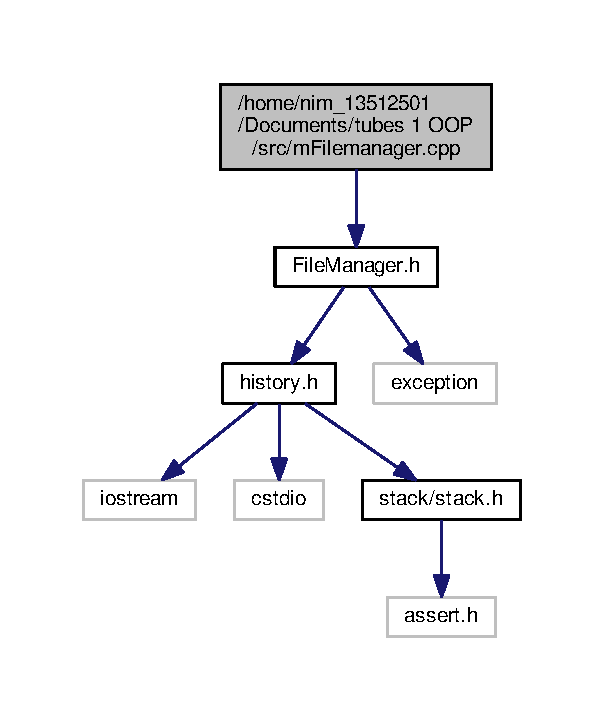
\includegraphics[width=290pt]{m_filemanager_8cpp__incl}
\end{center}
\end{figure}
\subsection*{Functions}
\begin{DoxyCompactItemize}
\item 
int \hyperlink{m_filemanager_8cpp_ae66f6b31b5ad750f1fe042a706a4e3d4}{main} ()
\begin{DoxyCompactList}\small\item\em test kelas \hyperlink{class_file_manager}{File\-Manager} \end{DoxyCompactList}\end{DoxyCompactItemize}


\subsection{Function Documentation}
\hypertarget{m_filemanager_8cpp_ae66f6b31b5ad750f1fe042a706a4e3d4}{\index{m\-Filemanager.\-cpp@{m\-Filemanager.\-cpp}!main@{main}}
\index{main@{main}!mFilemanager.cpp@{m\-Filemanager.\-cpp}}
\subsubsection[{main}]{\setlength{\rightskip}{0pt plus 5cm}int main (
\begin{DoxyParamCaption}
{}
\end{DoxyParamCaption}
)}}\label{m_filemanager_8cpp_ae66f6b31b5ad750f1fe042a706a4e3d4}


test kelas \hyperlink{class_file_manager}{File\-Manager} 


\hypertarget{mhistory_8cpp}{\section{/home/nim\-\_\-13512501/\-Documents/tubes 1 O\-O\-P/src/mhistory.cpp File Reference}
\label{mhistory_8cpp}\index{/home/nim\-\_\-13512501/\-Documents/tubes 1 O\-O\-P/src/mhistory.\-cpp@{/home/nim\-\_\-13512501/\-Documents/tubes 1 O\-O\-P/src/mhistory.\-cpp}}
}
{\ttfamily \#include $<$iostream$>$}\\*
{\ttfamily \#include $<$cstdio$>$}\\*
{\ttfamily \#include $<$cassert$>$}\\*
{\ttfamily \#include \char`\"{}history.\-h\char`\"{}}\\*
Include dependency graph for mhistory.\-cpp\-:\nopagebreak
\begin{figure}[H]
\begin{center}
\leavevmode
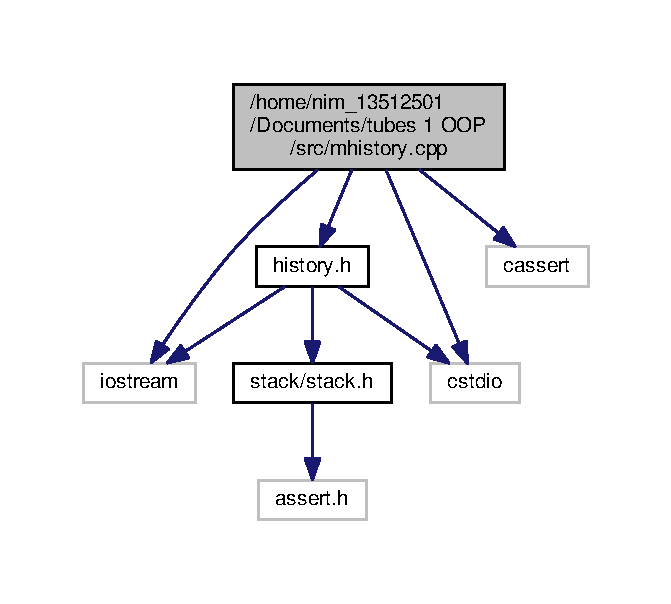
\includegraphics[width=322pt]{mhistory_8cpp__incl}
\end{center}
\end{figure}
\subsection*{Functions}
\begin{DoxyCompactItemize}
\item 
int \hyperlink{mhistory_8cpp_ae66f6b31b5ad750f1fe042a706a4e3d4}{main} ()
\end{DoxyCompactItemize}


\subsection{Function Documentation}
\hypertarget{mhistory_8cpp_ae66f6b31b5ad750f1fe042a706a4e3d4}{\index{mhistory.\-cpp@{mhistory.\-cpp}!main@{main}}
\index{main@{main}!mhistory.cpp@{mhistory.\-cpp}}
\subsubsection[{main}]{\setlength{\rightskip}{0pt plus 5cm}int main (
\begin{DoxyParamCaption}
{}
\end{DoxyParamCaption}
)}}\label{mhistory_8cpp_ae66f6b31b5ad750f1fe042a706a4e3d4}

\hypertarget{m_u_i_8cpp}{\section{/home/nim\-\_\-13512501/\-Documents/tubes 1 O\-O\-P/src/m\-U\-I.cpp File Reference}
\label{m_u_i_8cpp}\index{/home/nim\-\_\-13512501/\-Documents/tubes 1 O\-O\-P/src/m\-U\-I.\-cpp@{/home/nim\-\_\-13512501/\-Documents/tubes 1 O\-O\-P/src/m\-U\-I.\-cpp}}
}
{\ttfamily \#include \char`\"{}U\-I.\-h\char`\"{}}\\*
Include dependency graph for m\-U\-I.\-cpp\-:\nopagebreak
\begin{figure}[H]
\begin{center}
\leavevmode
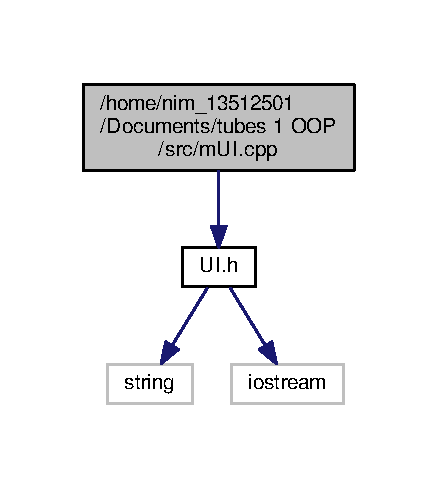
\includegraphics[width=210pt]{m_u_i_8cpp__incl}
\end{center}
\end{figure}
\subsection*{Functions}
\begin{DoxyCompactItemize}
\item 
int \hyperlink{m_u_i_8cpp_ae66f6b31b5ad750f1fe042a706a4e3d4}{main} ()
\begin{DoxyCompactList}\small\item\em test kelas \hyperlink{class_u_i}{U\-I} \end{DoxyCompactList}\end{DoxyCompactItemize}


\subsection{Function Documentation}
\hypertarget{m_u_i_8cpp_ae66f6b31b5ad750f1fe042a706a4e3d4}{\index{m\-U\-I.\-cpp@{m\-U\-I.\-cpp}!main@{main}}
\index{main@{main}!mUI.cpp@{m\-U\-I.\-cpp}}
\subsubsection[{main}]{\setlength{\rightskip}{0pt plus 5cm}int main (
\begin{DoxyParamCaption}
{}
\end{DoxyParamCaption}
)}}\label{m_u_i_8cpp_ae66f6b31b5ad750f1fe042a706a4e3d4}


test kelas \hyperlink{class_u_i}{U\-I} 


\hypertarget{mstack_8cpp}{\section{/home/nim\-\_\-13512501/\-Documents/tubes 1 O\-O\-P/src/stack/mstack.cpp File Reference}
\label{mstack_8cpp}\index{/home/nim\-\_\-13512501/\-Documents/tubes 1 O\-O\-P/src/stack/mstack.\-cpp@{/home/nim\-\_\-13512501/\-Documents/tubes 1 O\-O\-P/src/stack/mstack.\-cpp}}
}
{\ttfamily \#include \char`\"{}stack.\-h\char`\"{}}\\*
{\ttfamily \#include $<$cassert$>$}\\*
{\ttfamily \#include $<$iostream$>$}\\*
Include dependency graph for mstack.\-cpp\-:\nopagebreak
\begin{figure}[H]
\begin{center}
\leavevmode
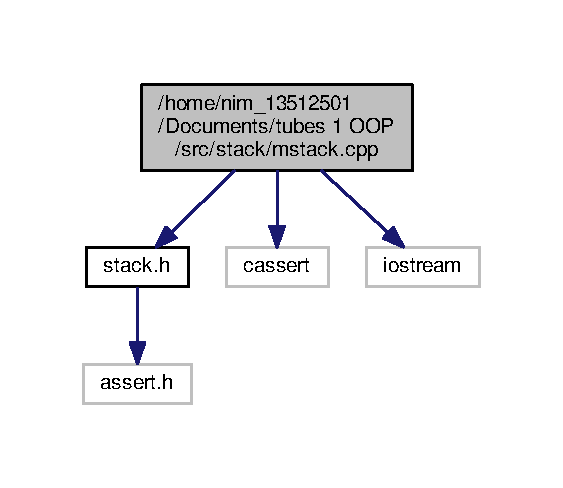
\includegraphics[width=270pt]{mstack_8cpp__incl}
\end{center}
\end{figure}
\subsection*{Functions}
\begin{DoxyCompactItemize}
\item 
int \hyperlink{mstack_8cpp_ae66f6b31b5ad750f1fe042a706a4e3d4}{main} ()
\end{DoxyCompactItemize}


\subsection{Function Documentation}
\hypertarget{mstack_8cpp_ae66f6b31b5ad750f1fe042a706a4e3d4}{\index{mstack.\-cpp@{mstack.\-cpp}!main@{main}}
\index{main@{main}!mstack.cpp@{mstack.\-cpp}}
\subsubsection[{main}]{\setlength{\rightskip}{0pt plus 5cm}int main (
\begin{DoxyParamCaption}
{}
\end{DoxyParamCaption}
)}}\label{mstack_8cpp_ae66f6b31b5ad750f1fe042a706a4e3d4}

\hypertarget{stack_8h}{\section{/home/nim\-\_\-13512501/\-Documents/tubes 1 O\-O\-P/src/stack/stack.h File Reference}
\label{stack_8h}\index{/home/nim\-\_\-13512501/\-Documents/tubes 1 O\-O\-P/src/stack/stack.\-h@{/home/nim\-\_\-13512501/\-Documents/tubes 1 O\-O\-P/src/stack/stack.\-h}}
}
{\ttfamily \#include $<$assert.\-h$>$}\\*
Include dependency graph for stack.\-h\-:\nopagebreak
\begin{figure}[H]
\begin{center}
\leavevmode
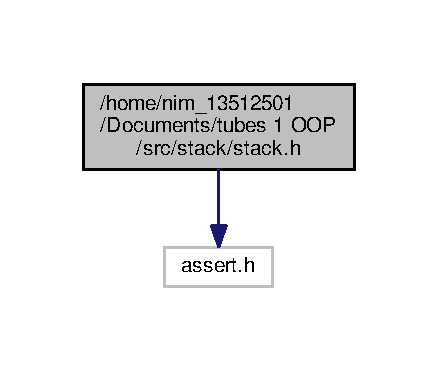
\includegraphics[width=210pt]{stack_8h__incl}
\end{center}
\end{figure}
This graph shows which files directly or indirectly include this file\-:\nopagebreak
\begin{figure}[H]
\begin{center}
\leavevmode
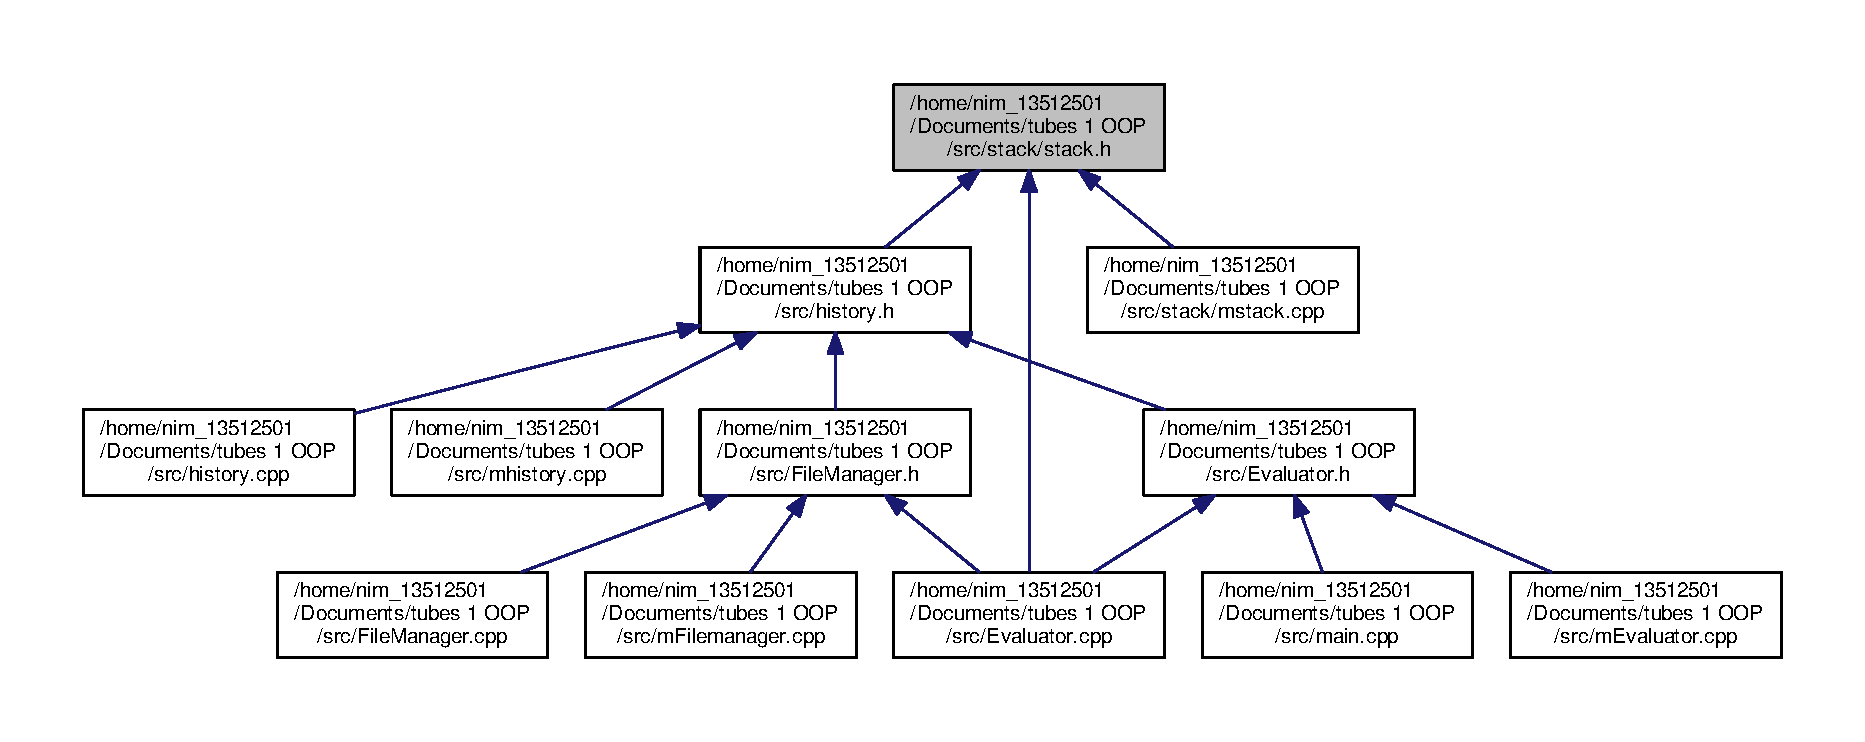
\includegraphics[width=350pt]{stack_8h__dep__incl}
\end{center}
\end{figure}
\subsection*{Classes}
\begin{DoxyCompactItemize}
\item 
class \hyperlink{class_stack}{Stack$<$ T $>$}
\end{DoxyCompactItemize}

\hypertarget{_arab_8cpp}{\section{/home/nim\-\_\-13512501/\-Documents/tubes 1 O\-O\-P/src/token/\-Arab.cpp File Reference}
\label{_arab_8cpp}\index{/home/nim\-\_\-13512501/\-Documents/tubes 1 O\-O\-P/src/token/\-Arab.\-cpp@{/home/nim\-\_\-13512501/\-Documents/tubes 1 O\-O\-P/src/token/\-Arab.\-cpp}}
}
{\ttfamily \#include \char`\"{}Arab.\-h\char`\"{}}\\*
{\ttfamily \#include $<$sstream$>$}\\*
{\ttfamily \#include $<$climits$>$}\\*
{\ttfamily \#include $<$cmath$>$}\\*
Include dependency graph for Arab.\-cpp\-:\nopagebreak
\begin{figure}[H]
\begin{center}
\leavevmode
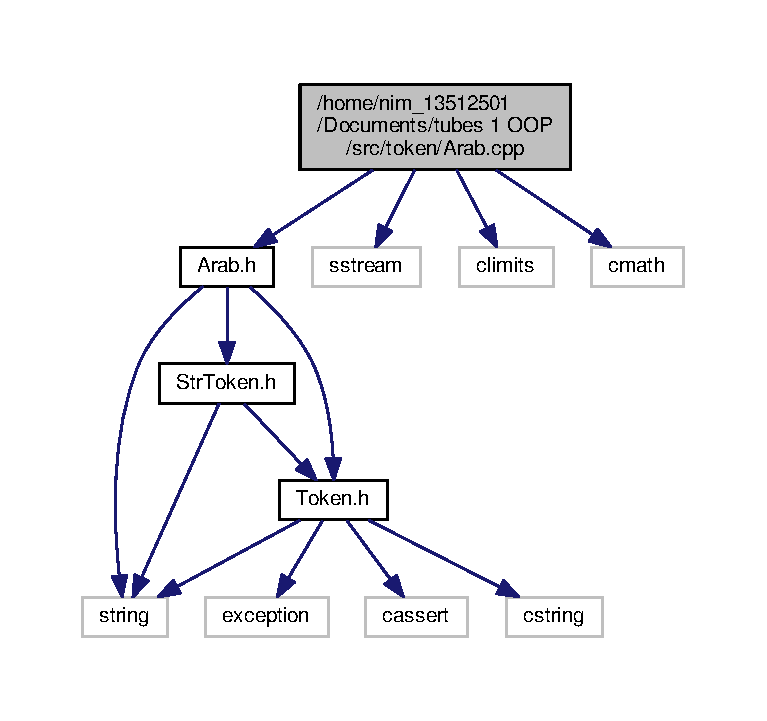
\includegraphics[width=350pt]{_arab_8cpp__incl}
\end{center}
\end{figure}

\hypertarget{_arab_8h}{\section{/home/nim\-\_\-13512501/\-Documents/tubes 1 O\-O\-P/src/token/\-Arab.h File Reference}
\label{_arab_8h}\index{/home/nim\-\_\-13512501/\-Documents/tubes 1 O\-O\-P/src/token/\-Arab.\-h@{/home/nim\-\_\-13512501/\-Documents/tubes 1 O\-O\-P/src/token/\-Arab.\-h}}
}
{\ttfamily \#include $<$string$>$}\\*
{\ttfamily \#include \char`\"{}Token.\-h\char`\"{}}\\*
{\ttfamily \#include \char`\"{}Str\-Token.\-h\char`\"{}}\\*
Include dependency graph for Arab.\-h\-:\nopagebreak
\begin{figure}[H]
\begin{center}
\leavevmode
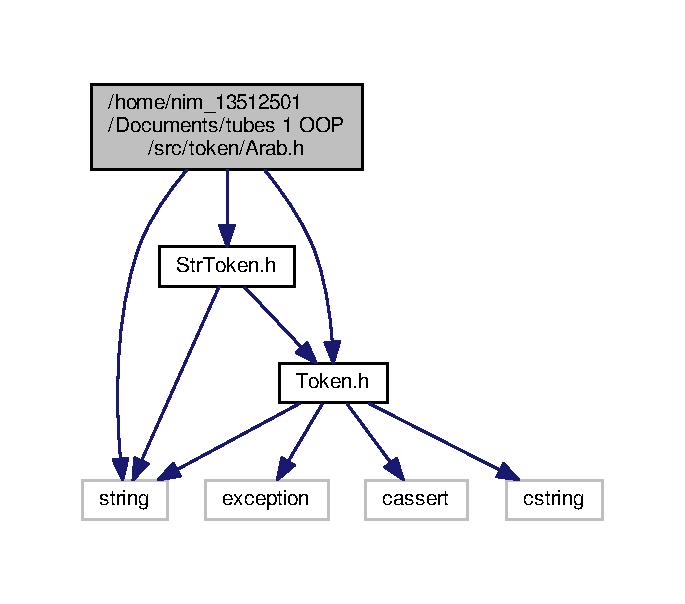
\includegraphics[width=329pt]{_arab_8h__incl}
\end{center}
\end{figure}
This graph shows which files directly or indirectly include this file\-:\nopagebreak
\begin{figure}[H]
\begin{center}
\leavevmode
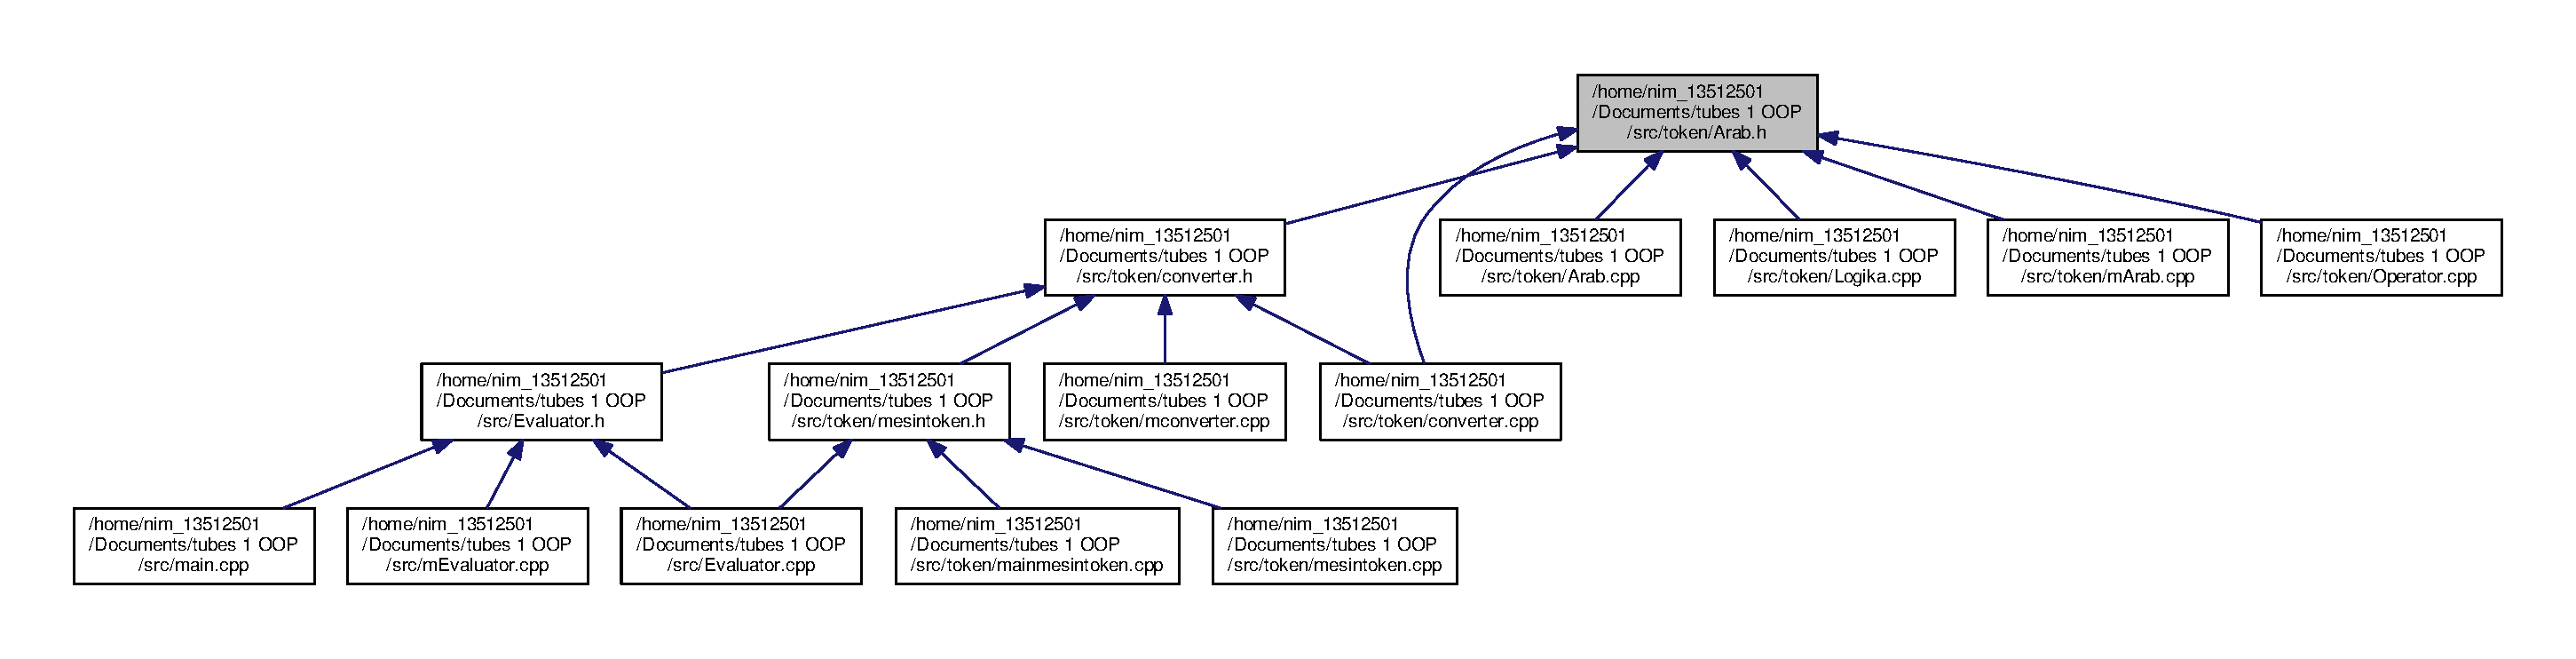
\includegraphics[width=350pt]{_arab_8h__dep__incl}
\end{center}
\end{figure}
\subsection*{Classes}
\begin{DoxyCompactItemize}
\item 
class \hyperlink{class_arab}{Arab}
\end{DoxyCompactItemize}

\hypertarget{converter_8cpp}{\section{/home/nim\-\_\-13512501/\-Documents/tubes 1 O\-O\-P/src/token/converter.cpp File Reference}
\label{converter_8cpp}\index{/home/nim\-\_\-13512501/\-Documents/tubes 1 O\-O\-P/src/token/converter.\-cpp@{/home/nim\-\_\-13512501/\-Documents/tubes 1 O\-O\-P/src/token/converter.\-cpp}}
}
{\ttfamily \#include \char`\"{}converter.\-h\char`\"{}}\\*
{\ttfamily \#include \char`\"{}Arab.\-h\char`\"{}}\\*
{\ttfamily \#include $<$cassert$>$}\\*
Include dependency graph for converter.\-cpp\-:\nopagebreak
\begin{figure}[H]
\begin{center}
\leavevmode
\includegraphics[width=350pt]{converter_8cpp__incl}
\end{center}
\end{figure}

\hypertarget{converter_8h}{\section{/home/nim\-\_\-13512501/\-Documents/tubes 1 O\-O\-P/src/token/converter.h File Reference}
\label{converter_8h}\index{/home/nim\-\_\-13512501/\-Documents/tubes 1 O\-O\-P/src/token/converter.\-h@{/home/nim\-\_\-13512501/\-Documents/tubes 1 O\-O\-P/src/token/converter.\-h}}
}
{\ttfamily \#include $<$exception$>$}\\*
{\ttfamily \#include $<$string$>$}\\*
{\ttfamily \#include \char`\"{}Token.\-h\char`\"{}}\\*
{\ttfamily \#include \char`\"{}Str\-Token.\-h\char`\"{}}\\*
{\ttfamily \#include \char`\"{}Arab.\-h\char`\"{}}\\*
{\ttfamily \#include \char`\"{}Logika.\-h\char`\"{}}\\*
{\ttfamily \#include \char`\"{}Operator.\-h\char`\"{}}\\*
{\ttfamily \#include \char`\"{}Romawi.\-h\char`\"{}}\\*
Include dependency graph for converter.\-h\-:\nopagebreak
\begin{figure}[H]
\begin{center}
\leavevmode
\includegraphics[width=350pt]{converter_8h__incl}
\end{center}
\end{figure}
This graph shows which files directly or indirectly include this file\-:\nopagebreak
\begin{figure}[H]
\begin{center}
\leavevmode
\includegraphics[width=350pt]{converter_8h__dep__incl}
\end{center}
\end{figure}
\subsection*{Classes}
\begin{DoxyCompactItemize}
\item 
class \hyperlink{class_converter}{Converter}
\item 
class \hyperlink{class_converter_exception}{Converter\-Exception}
\end{DoxyCompactItemize}

\hypertarget{_logika_8cpp}{\section{/home/nim\-\_\-13512501/\-Documents/tubes 1 O\-O\-P/src/token/\-Logika.cpp File Reference}
\label{_logika_8cpp}\index{/home/nim\-\_\-13512501/\-Documents/tubes 1 O\-O\-P/src/token/\-Logika.\-cpp@{/home/nim\-\_\-13512501/\-Documents/tubes 1 O\-O\-P/src/token/\-Logika.\-cpp}}
}
{\ttfamily \#include \char`\"{}Logika.\-h\char`\"{}}\\*
{\ttfamily \#include \char`\"{}Arab.\-h\char`\"{}}\\*
{\ttfamily \#include $<$sstream$>$}\\*
Include dependency graph for Logika.\-cpp\-:\nopagebreak
\begin{figure}[H]
\begin{center}
\leavevmode
\includegraphics[width=350pt]{_logika_8cpp__incl}
\end{center}
\end{figure}

\hypertarget{_logika_8h}{\section{/home/nim\-\_\-13512501/\-Documents/tubes 1 O\-O\-P/src/token/\-Logika.h File Reference}
\label{_logika_8h}\index{/home/nim\-\_\-13512501/\-Documents/tubes 1 O\-O\-P/src/token/\-Logika.\-h@{/home/nim\-\_\-13512501/\-Documents/tubes 1 O\-O\-P/src/token/\-Logika.\-h}}
}
{\ttfamily \#include $<$string$>$}\\*
{\ttfamily \#include \char`\"{}Token.\-h\char`\"{}}\\*
{\ttfamily \#include \char`\"{}Str\-Token.\-h\char`\"{}}\\*
Include dependency graph for Logika.\-h\-:\nopagebreak
\begin{figure}[H]
\begin{center}
\leavevmode
\includegraphics[width=329pt]{_logika_8h__incl}
\end{center}
\end{figure}
This graph shows which files directly or indirectly include this file\-:\nopagebreak
\begin{figure}[H]
\begin{center}
\leavevmode
\includegraphics[width=350pt]{_logika_8h__dep__incl}
\end{center}
\end{figure}
\subsection*{Classes}
\begin{DoxyCompactItemize}
\item 
class \hyperlink{class_logika}{Logika}
\end{DoxyCompactItemize}

\hypertarget{mainmesintoken_8cpp}{\section{/home/nim\-\_\-13512501/\-Documents/tubes 1 O\-O\-P/src/token/mainmesintoken.cpp File Reference}
\label{mainmesintoken_8cpp}\index{/home/nim\-\_\-13512501/\-Documents/tubes 1 O\-O\-P/src/token/mainmesintoken.\-cpp@{/home/nim\-\_\-13512501/\-Documents/tubes 1 O\-O\-P/src/token/mainmesintoken.\-cpp}}
}
{\ttfamily \#include \char`\"{}mesintoken.\-h\char`\"{}}\\*
{\ttfamily \#include $<$string$>$}\\*
{\ttfamily \#include $<$iostream$>$}\\*
Include dependency graph for mainmesintoken.\-cpp\-:\nopagebreak
\begin{figure}[H]
\begin{center}
\leavevmode
\includegraphics[width=350pt]{mainmesintoken_8cpp__incl}
\end{center}
\end{figure}
\subsection*{Functions}
\begin{DoxyCompactItemize}
\item 
int \hyperlink{mainmesintoken_8cpp_ae66f6b31b5ad750f1fe042a706a4e3d4}{main} ()
\begin{DoxyCompactList}\small\item\em test mesin token \end{DoxyCompactList}\end{DoxyCompactItemize}


\subsection{Function Documentation}
\hypertarget{mainmesintoken_8cpp_ae66f6b31b5ad750f1fe042a706a4e3d4}{\index{mainmesintoken.\-cpp@{mainmesintoken.\-cpp}!main@{main}}
\index{main@{main}!mainmesintoken.cpp@{mainmesintoken.\-cpp}}
\subsubsection[{main}]{\setlength{\rightskip}{0pt plus 5cm}int main (
\begin{DoxyParamCaption}
{}
\end{DoxyParamCaption}
)}}\label{mainmesintoken_8cpp_ae66f6b31b5ad750f1fe042a706a4e3d4}


test mesin token 


\hypertarget{m_arab_8cpp}{\section{/home/nim\-\_\-13512501/\-Documents/tubes 1 O\-O\-P/src/token/m\-Arab.cpp File Reference}
\label{m_arab_8cpp}\index{/home/nim\-\_\-13512501/\-Documents/tubes 1 O\-O\-P/src/token/m\-Arab.\-cpp@{/home/nim\-\_\-13512501/\-Documents/tubes 1 O\-O\-P/src/token/m\-Arab.\-cpp}}
}
{\ttfamily \#include \char`\"{}Arab.\-h\char`\"{}}\\*
{\ttfamily \#include \char`\"{}Str\-Token.\-h\char`\"{}}\\*
{\ttfamily \#include $<$iostream$>$}\\*
Include dependency graph for m\-Arab.\-cpp\-:\nopagebreak
\begin{figure}[H]
\begin{center}
\leavevmode
\includegraphics[width=329pt]{m_arab_8cpp__incl}
\end{center}
\end{figure}
\subsection*{Functions}
\begin{DoxyCompactItemize}
\item 
int \hyperlink{m_arab_8cpp_ae66f6b31b5ad750f1fe042a706a4e3d4}{main} ()
\end{DoxyCompactItemize}


\subsection{Function Documentation}
\hypertarget{m_arab_8cpp_ae66f6b31b5ad750f1fe042a706a4e3d4}{\index{m\-Arab.\-cpp@{m\-Arab.\-cpp}!main@{main}}
\index{main@{main}!mArab.cpp@{m\-Arab.\-cpp}}
\subsubsection[{main}]{\setlength{\rightskip}{0pt plus 5cm}int main (
\begin{DoxyParamCaption}
{}
\end{DoxyParamCaption}
)}}\label{m_arab_8cpp_ae66f6b31b5ad750f1fe042a706a4e3d4}
test Kelas \hyperlink{class_arab}{Arab} 
\hypertarget{mconverter_8cpp}{\section{/home/nim\-\_\-13512501/\-Documents/tubes 1 O\-O\-P/src/token/mconverter.cpp File Reference}
\label{mconverter_8cpp}\index{/home/nim\-\_\-13512501/\-Documents/tubes 1 O\-O\-P/src/token/mconverter.\-cpp@{/home/nim\-\_\-13512501/\-Documents/tubes 1 O\-O\-P/src/token/mconverter.\-cpp}}
}
{\ttfamily \#include \char`\"{}converter.\-h\char`\"{}}\\*
{\ttfamily \#include $<$iostream$>$}\\*
Include dependency graph for mconverter.\-cpp\-:\nopagebreak
\begin{figure}[H]
\begin{center}
\leavevmode
\includegraphics[width=350pt]{mconverter_8cpp__incl}
\end{center}
\end{figure}
\subsection*{Functions}
\begin{DoxyCompactItemize}
\item 
int \hyperlink{mconverter_8cpp_ae66f6b31b5ad750f1fe042a706a4e3d4}{main} ()
\end{DoxyCompactItemize}


\subsection{Function Documentation}
\hypertarget{mconverter_8cpp_ae66f6b31b5ad750f1fe042a706a4e3d4}{\index{mconverter.\-cpp@{mconverter.\-cpp}!main@{main}}
\index{main@{main}!mconverter.cpp@{mconverter.\-cpp}}
\subsubsection[{main}]{\setlength{\rightskip}{0pt plus 5cm}int main (
\begin{DoxyParamCaption}
{}
\end{DoxyParamCaption}
)}}\label{mconverter_8cpp_ae66f6b31b5ad750f1fe042a706a4e3d4}
test untuk kelas \hyperlink{class_converter}{Converter} 
\hypertarget{mesintoken_8cpp}{\section{/home/nim\-\_\-13512501/\-Documents/tubes 1 O\-O\-P/src/token/mesintoken.cpp File Reference}
\label{mesintoken_8cpp}\index{/home/nim\-\_\-13512501/\-Documents/tubes 1 O\-O\-P/src/token/mesintoken.\-cpp@{/home/nim\-\_\-13512501/\-Documents/tubes 1 O\-O\-P/src/token/mesintoken.\-cpp}}
}
{\ttfamily \#include \char`\"{}mesintoken.\-h\char`\"{}}\\*
{\ttfamily \#include $<$cassert$>$}\\*
Include dependency graph for mesintoken.\-cpp\-:\nopagebreak
\begin{figure}[H]
\begin{center}
\leavevmode
\includegraphics[width=350pt]{mesintoken_8cpp__incl}
\end{center}
\end{figure}

\hypertarget{mesintoken_8h}{\section{/home/nim\-\_\-13512501/\-Documents/tubes 1 O\-O\-P/src/token/mesintoken.h File Reference}
\label{mesintoken_8h}\index{/home/nim\-\_\-13512501/\-Documents/tubes 1 O\-O\-P/src/token/mesintoken.\-h@{/home/nim\-\_\-13512501/\-Documents/tubes 1 O\-O\-P/src/token/mesintoken.\-h}}
}
{\ttfamily \#include \char`\"{}mesinkata.\-h\char`\"{}}\\*
{\ttfamily \#include \char`\"{}Token.\-h\char`\"{}}\\*
{\ttfamily \#include \char`\"{}converter.\-h\char`\"{}}\\*
{\ttfamily \#include $<$string$>$}\\*
Include dependency graph for mesintoken.\-h\-:\nopagebreak
\begin{figure}[H]
\begin{center}
\leavevmode
\includegraphics[width=350pt]{mesintoken_8h__incl}
\end{center}
\end{figure}
This graph shows which files directly or indirectly include this file\-:\nopagebreak
\begin{figure}[H]
\begin{center}
\leavevmode
\includegraphics[width=350pt]{mesintoken_8h__dep__incl}
\end{center}
\end{figure}
\subsection*{Classes}
\begin{DoxyCompactItemize}
\item 
class \hyperlink{classmesintoken}{mesintoken}
\end{DoxyCompactItemize}

\hypertarget{m_logika_8cpp}{\section{/home/nim\-\_\-13512501/\-Documents/tubes 1 O\-O\-P/src/token/m\-Logika.cpp File Reference}
\label{m_logika_8cpp}\index{/home/nim\-\_\-13512501/\-Documents/tubes 1 O\-O\-P/src/token/m\-Logika.\-cpp@{/home/nim\-\_\-13512501/\-Documents/tubes 1 O\-O\-P/src/token/m\-Logika.\-cpp}}
}
{\ttfamily \#include \char`\"{}Logika.\-h\char`\"{}}\\*
{\ttfamily \#include \char`\"{}Str\-Token.\-h\char`\"{}}\\*
{\ttfamily \#include $<$iostream$>$}\\*
Include dependency graph for m\-Logika.\-cpp\-:\nopagebreak
\begin{figure}[H]
\begin{center}
\leavevmode
\includegraphics[width=329pt]{m_logika_8cpp__incl}
\end{center}
\end{figure}
\subsection*{Functions}
\begin{DoxyCompactItemize}
\item 
int \hyperlink{m_logika_8cpp_ae66f6b31b5ad750f1fe042a706a4e3d4}{main} ()
\end{DoxyCompactItemize}


\subsection{Function Documentation}
\hypertarget{m_logika_8cpp_ae66f6b31b5ad750f1fe042a706a4e3d4}{\index{m\-Logika.\-cpp@{m\-Logika.\-cpp}!main@{main}}
\index{main@{main}!mLogika.cpp@{m\-Logika.\-cpp}}
\subsubsection[{main}]{\setlength{\rightskip}{0pt plus 5cm}int main (
\begin{DoxyParamCaption}
{}
\end{DoxyParamCaption}
)}}\label{m_logika_8cpp_ae66f6b31b5ad750f1fe042a706a4e3d4}
test kelas \hyperlink{class_logika}{Logika} 
\hypertarget{m_operator_8cpp}{\section{/home/nim\-\_\-13512501/\-Documents/tubes 1 O\-O\-P/src/token/m\-Operator.cpp File Reference}
\label{m_operator_8cpp}\index{/home/nim\-\_\-13512501/\-Documents/tubes 1 O\-O\-P/src/token/m\-Operator.\-cpp@{/home/nim\-\_\-13512501/\-Documents/tubes 1 O\-O\-P/src/token/m\-Operator.\-cpp}}
}
{\ttfamily \#include \char`\"{}Operator.\-h\char`\"{}}\\*
{\ttfamily \#include $<$iostream$>$}\\*
Include dependency graph for m\-Operator.\-cpp\-:\nopagebreak
\begin{figure}[H]
\begin{center}
\leavevmode
\includegraphics[width=329pt]{m_operator_8cpp__incl}
\end{center}
\end{figure}
\subsection*{Functions}
\begin{DoxyCompactItemize}
\item 
int \hyperlink{m_operator_8cpp_ae66f6b31b5ad750f1fe042a706a4e3d4}{main} ()
\end{DoxyCompactItemize}


\subsection{Function Documentation}
\hypertarget{m_operator_8cpp_ae66f6b31b5ad750f1fe042a706a4e3d4}{\index{m\-Operator.\-cpp@{m\-Operator.\-cpp}!main@{main}}
\index{main@{main}!mOperator.cpp@{m\-Operator.\-cpp}}
\subsubsection[{main}]{\setlength{\rightskip}{0pt plus 5cm}int main (
\begin{DoxyParamCaption}
{}
\end{DoxyParamCaption}
)}}\label{m_operator_8cpp_ae66f6b31b5ad750f1fe042a706a4e3d4}
test kelas \hyperlink{class_operator}{Operator} 
\hypertarget{m_romawi_8cpp}{\section{/home/nim\-\_\-13512501/\-Documents/tubes 1 O\-O\-P/src/token/m\-Romawi.cpp File Reference}
\label{m_romawi_8cpp}\index{/home/nim\-\_\-13512501/\-Documents/tubes 1 O\-O\-P/src/token/m\-Romawi.\-cpp@{/home/nim\-\_\-13512501/\-Documents/tubes 1 O\-O\-P/src/token/m\-Romawi.\-cpp}}
}
{\ttfamily \#include \char`\"{}Romawi.\-h\char`\"{}}\\*
{\ttfamily \#include \char`\"{}Str\-Token.\-h\char`\"{}}\\*
{\ttfamily \#include $<$iostream$>$}\\*
Include dependency graph for m\-Romawi.\-cpp\-:\nopagebreak
\begin{figure}[H]
\begin{center}
\leavevmode
\includegraphics[width=329pt]{m_romawi_8cpp__incl}
\end{center}
\end{figure}
\subsection*{Functions}
\begin{DoxyCompactItemize}
\item 
int \hyperlink{m_romawi_8cpp_ae66f6b31b5ad750f1fe042a706a4e3d4}{main} ()
\begin{DoxyCompactList}\small\item\em test untuk kelas \hyperlink{class_romawi}{Romawi} \end{DoxyCompactList}\end{DoxyCompactItemize}


\subsection{Function Documentation}
\hypertarget{m_romawi_8cpp_ae66f6b31b5ad750f1fe042a706a4e3d4}{\index{m\-Romawi.\-cpp@{m\-Romawi.\-cpp}!main@{main}}
\index{main@{main}!mRomawi.cpp@{m\-Romawi.\-cpp}}
\subsubsection[{main}]{\setlength{\rightskip}{0pt plus 5cm}int main (
\begin{DoxyParamCaption}
{}
\end{DoxyParamCaption}
)}}\label{m_romawi_8cpp_ae66f6b31b5ad750f1fe042a706a4e3d4}


test untuk kelas \hyperlink{class_romawi}{Romawi} 


\hypertarget{m_token_8cpp}{\section{/home/nim\-\_\-13512501/\-Documents/tubes 1 O\-O\-P/src/token/m\-Token.cpp File Reference}
\label{m_token_8cpp}\index{/home/nim\-\_\-13512501/\-Documents/tubes 1 O\-O\-P/src/token/m\-Token.\-cpp@{/home/nim\-\_\-13512501/\-Documents/tubes 1 O\-O\-P/src/token/m\-Token.\-cpp}}
}
{\ttfamily \#include \char`\"{}Token.\-h\char`\"{}}\\*
{\ttfamily \#include $<$iostream$>$}\\*
{\ttfamily \#include $<$limits$>$}\\*
{\ttfamily \#include $<$climits$>$}\\*
{\ttfamily \#include $<$cfloat$>$}\\*
{\ttfamily \#include $<$cstdlib$>$}\\*
{\ttfamily \#include $<$ctime$>$}\\*
Include dependency graph for m\-Token.\-cpp\-:\nopagebreak
\begin{figure}[H]
\begin{center}
\leavevmode
\includegraphics[width=350pt]{m_token_8cpp__incl}
\end{center}
\end{figure}
\subsection*{Functions}
\begin{DoxyCompactItemize}
\item 
int \hyperlink{m_token_8cpp_ae66f6b31b5ad750f1fe042a706a4e3d4}{main} ()
\begin{DoxyCompactList}\small\item\em test untuk kelas \hyperlink{class_token}{Token} \end{DoxyCompactList}\end{DoxyCompactItemize}


\subsection{Function Documentation}
\hypertarget{m_token_8cpp_ae66f6b31b5ad750f1fe042a706a4e3d4}{\index{m\-Token.\-cpp@{m\-Token.\-cpp}!main@{main}}
\index{main@{main}!mToken.cpp@{m\-Token.\-cpp}}
\subsubsection[{main}]{\setlength{\rightskip}{0pt plus 5cm}int main (
\begin{DoxyParamCaption}
{}
\end{DoxyParamCaption}
)}}\label{m_token_8cpp_ae66f6b31b5ad750f1fe042a706a4e3d4}


test untuk kelas \hyperlink{class_token}{Token} 


\hypertarget{_operator_8cpp}{\section{/home/nim\-\_\-13512501/\-Documents/tubes 1 O\-O\-P/src/token/\-Operator.cpp File Reference}
\label{_operator_8cpp}\index{/home/nim\-\_\-13512501/\-Documents/tubes 1 O\-O\-P/src/token/\-Operator.\-cpp@{/home/nim\-\_\-13512501/\-Documents/tubes 1 O\-O\-P/src/token/\-Operator.\-cpp}}
}
{\ttfamily \#include \char`\"{}Logika.\-h\char`\"{}}\\*
{\ttfamily \#include \char`\"{}Arab.\-h\char`\"{}}\\*
{\ttfamily \#include \char`\"{}Romawi.\-h\char`\"{}}\\*
{\ttfamily \#include \char`\"{}Operator.\-h\char`\"{}}\\*
{\ttfamily \#include $<$sstream$>$}\\*
{\ttfamily \#include $<$cassert$>$}\\*
Include dependency graph for Operator.\-cpp\-:\nopagebreak
\begin{figure}[H]
\begin{center}
\leavevmode
\includegraphics[width=350pt]{_operator_8cpp__incl}
\end{center}
\end{figure}

\hypertarget{_operator_8h}{\section{/home/nim\-\_\-13512501/\-Documents/tubes 1 O\-O\-P/src/token/\-Operator.h File Reference}
\label{_operator_8h}\index{/home/nim\-\_\-13512501/\-Documents/tubes 1 O\-O\-P/src/token/\-Operator.\-h@{/home/nim\-\_\-13512501/\-Documents/tubes 1 O\-O\-P/src/token/\-Operator.\-h}}
}
{\ttfamily \#include $<$string$>$}\\*
{\ttfamily \#include \char`\"{}Token.\-h\char`\"{}}\\*
{\ttfamily \#include \char`\"{}Str\-Token.\-h\char`\"{}}\\*
Include dependency graph for Operator.\-h\-:\nopagebreak
\begin{figure}[H]
\begin{center}
\leavevmode
\includegraphics[width=329pt]{_operator_8h__incl}
\end{center}
\end{figure}
This graph shows which files directly or indirectly include this file\-:\nopagebreak
\begin{figure}[H]
\begin{center}
\leavevmode
\includegraphics[width=350pt]{_operator_8h__dep__incl}
\end{center}
\end{figure}
\subsection*{Classes}
\begin{DoxyCompactItemize}
\item 
class \hyperlink{class_operator}{Operator}
\end{DoxyCompactItemize}
\subsection*{Macros}
\begin{DoxyCompactItemize}
\item 
\#define \hyperlink{_operator_8h_a8fe3adeb30ba32978aabe9d2ea870ef3}{T\-I\-P\-E\-T\-O\-K\-E\-N\-\_\-\-C\-O\-U\-N\-T}~12
\end{DoxyCompactItemize}


\subsection{Macro Definition Documentation}
\hypertarget{_operator_8h_a8fe3adeb30ba32978aabe9d2ea870ef3}{\index{Operator.\-h@{Operator.\-h}!T\-I\-P\-E\-T\-O\-K\-E\-N\-\_\-\-C\-O\-U\-N\-T@{T\-I\-P\-E\-T\-O\-K\-E\-N\-\_\-\-C\-O\-U\-N\-T}}
\index{T\-I\-P\-E\-T\-O\-K\-E\-N\-\_\-\-C\-O\-U\-N\-T@{T\-I\-P\-E\-T\-O\-K\-E\-N\-\_\-\-C\-O\-U\-N\-T}!Operator.h@{Operator.\-h}}
\subsubsection[{T\-I\-P\-E\-T\-O\-K\-E\-N\-\_\-\-C\-O\-U\-N\-T}]{\setlength{\rightskip}{0pt plus 5cm}\#define T\-I\-P\-E\-T\-O\-K\-E\-N\-\_\-\-C\-O\-U\-N\-T~12}}\label{_operator_8h_a8fe3adeb30ba32978aabe9d2ea870ef3}

\hypertarget{_romawi_8cpp}{\section{/home/nim\-\_\-13512501/\-Documents/tubes 1 O\-O\-P/src/token/\-Romawi.cpp File Reference}
\label{_romawi_8cpp}\index{/home/nim\-\_\-13512501/\-Documents/tubes 1 O\-O\-P/src/token/\-Romawi.\-cpp@{/home/nim\-\_\-13512501/\-Documents/tubes 1 O\-O\-P/src/token/\-Romawi.\-cpp}}
}
{\ttfamily \#include \char`\"{}Romawi.\-h\char`\"{}}\\*
{\ttfamily \#include $<$sstream$>$}\\*
{\ttfamily \#include $<$cmath$>$}\\*
{\ttfamily \#include $<$climits$>$}\\*
Include dependency graph for Romawi.\-cpp\-:\nopagebreak
\begin{figure}[H]
\begin{center}
\leavevmode
\includegraphics[width=350pt]{_romawi_8cpp__incl}
\end{center}
\end{figure}

\hypertarget{_romawi_8h}{\section{/home/nim\-\_\-13512501/\-Documents/tubes 1 O\-O\-P/src/token/\-Romawi.h File Reference}
\label{_romawi_8h}\index{/home/nim\-\_\-13512501/\-Documents/tubes 1 O\-O\-P/src/token/\-Romawi.\-h@{/home/nim\-\_\-13512501/\-Documents/tubes 1 O\-O\-P/src/token/\-Romawi.\-h}}
}
{\ttfamily \#include $<$string$>$}\\*
{\ttfamily \#include \char`\"{}Token.\-h\char`\"{}}\\*
{\ttfamily \#include \char`\"{}Str\-Token.\-h\char`\"{}}\\*
Include dependency graph for Romawi.\-h\-:\nopagebreak
\begin{figure}[H]
\begin{center}
\leavevmode
\includegraphics[width=329pt]{_romawi_8h__incl}
\end{center}
\end{figure}
This graph shows which files directly or indirectly include this file\-:\nopagebreak
\begin{figure}[H]
\begin{center}
\leavevmode
\includegraphics[width=350pt]{_romawi_8h__dep__incl}
\end{center}
\end{figure}
\subsection*{Classes}
\begin{DoxyCompactItemize}
\item 
class \hyperlink{class_romawi}{Romawi}
\begin{DoxyCompactList}\small\item\em kelas implementasi \hyperlink{class_str_token}{Str\-Token} dengan aturan representasi bilangan romawi \end{DoxyCompactList}\end{DoxyCompactItemize}

\hypertarget{_str_token_8h}{\section{/home/nim\-\_\-13512501/\-Documents/tubes 1 O\-O\-P/src/token/\-Str\-Token.h File Reference}
\label{_str_token_8h}\index{/home/nim\-\_\-13512501/\-Documents/tubes 1 O\-O\-P/src/token/\-Str\-Token.\-h@{/home/nim\-\_\-13512501/\-Documents/tubes 1 O\-O\-P/src/token/\-Str\-Token.\-h}}
}
{\ttfamily \#include $<$string$>$}\\*
{\ttfamily \#include \char`\"{}Token.\-h\char`\"{}}\\*
Include dependency graph for Str\-Token.\-h\-:\nopagebreak
\begin{figure}[H]
\begin{center}
\leavevmode
\includegraphics[width=333pt]{_str_token_8h__incl}
\end{center}
\end{figure}
This graph shows which files directly or indirectly include this file\-:\nopagebreak
\begin{figure}[H]
\begin{center}
\leavevmode
\includegraphics[width=350pt]{_str_token_8h__dep__incl}
\end{center}
\end{figure}
\subsection*{Classes}
\begin{DoxyCompactItemize}
\item 
class \hyperlink{class_str_token}{Str\-Token}
\end{DoxyCompactItemize}

\hypertarget{_token_8cpp}{\section{/home/nim\-\_\-13512501/\-Documents/tubes 1 O\-O\-P/src/token/\-Token.cpp File Reference}
\label{_token_8cpp}\index{/home/nim\-\_\-13512501/\-Documents/tubes 1 O\-O\-P/src/token/\-Token.\-cpp@{/home/nim\-\_\-13512501/\-Documents/tubes 1 O\-O\-P/src/token/\-Token.\-cpp}}
}
{\ttfamily \#include \char`\"{}Token.\-h\char`\"{}}\\*
{\ttfamily \#include $<$cassert$>$}\\*
{\ttfamily \#include $<$climits$>$}\\*
{\ttfamily \#include $<$cmath$>$}\\*
{\ttfamily \#include $<$iostream$>$}\\*
{\ttfamily \#include $<$cstring$>$}\\*
{\ttfamily \#include $<$sstream$>$}\\*
Include dependency graph for Token.\-cpp\-:\nopagebreak
\begin{figure}[H]
\begin{center}
\leavevmode
\includegraphics[width=350pt]{_token_8cpp__incl}
\end{center}
\end{figure}

\hypertarget{_token_8h}{\section{/home/nim\-\_\-13512501/\-Documents/tubes 1 O\-O\-P/src/token/\-Token.h File Reference}
\label{_token_8h}\index{/home/nim\-\_\-13512501/\-Documents/tubes 1 O\-O\-P/src/token/\-Token.\-h@{/home/nim\-\_\-13512501/\-Documents/tubes 1 O\-O\-P/src/token/\-Token.\-h}}
}
{\ttfamily \#include $<$string$>$}\\*
{\ttfamily \#include $<$exception$>$}\\*
{\ttfamily \#include $<$cassert$>$}\\*
{\ttfamily \#include $<$cstring$>$}\\*
Include dependency graph for Token.\-h\-:\nopagebreak
\begin{figure}[H]
\begin{center}
\leavevmode
\includegraphics[width=329pt]{_token_8h__incl}
\end{center}
\end{figure}
This graph shows which files directly or indirectly include this file\-:\nopagebreak
\begin{figure}[H]
\begin{center}
\leavevmode
\includegraphics[width=350pt]{_token_8h__dep__incl}
\end{center}
\end{figure}
\subsection*{Classes}
\begin{DoxyCompactItemize}
\item 
class \hyperlink{class_token}{Token}
\item 
class \hyperlink{class_token_exception}{Token\-Exception}
\end{DoxyCompactItemize}
\subsection*{Enumerations}
\begin{DoxyCompactItemize}
\item 
enum \hyperlink{_token_8h_a29ea73031d51befacf649fa6af865e30}{Tipe\-Token} \{ \\*
\hyperlink{_token_8h_a29ea73031d51befacf649fa6af865e30ac81f835bf8ff78b7a9057198c13a0614}{Kali}, 
\hyperlink{_token_8h_a29ea73031d51befacf649fa6af865e30a496e53e4414f86be15b33646c2239575}{Bagi}, 
\hyperlink{_token_8h_a29ea73031d51befacf649fa6af865e30af8a422934e5f1fb7651b81fc0693648c}{Tambah}, 
\hyperlink{_token_8h_a29ea73031d51befacf649fa6af865e30a3b838967b6091702ffe978675fce0cc6}{Kurang}, 
\\*
\hyperlink{_token_8h_a29ea73031d51befacf649fa6af865e30ae6fac012a9b23f2f87d8094e349e4418}{Div}, 
\hyperlink{_token_8h_a29ea73031d51befacf649fa6af865e30a6265a10e42e4cfbf0c109d1685551e38}{Mod}, 
\hyperlink{_token_8h_a29ea73031d51befacf649fa6af865e30a68a4e1b7240c2549f862bc0bbeadd13f}{Kurungbuka}, 
\hyperlink{_token_8h_a29ea73031d51befacf649fa6af865e30aa4bab5df91578b528627ef4a8595da2d}{Kurungtutup}, 
\\*
\hyperlink{_token_8h_a29ea73031d51befacf649fa6af865e30a60b042c2c7da21af2ed42f8cc27e7ff8}{And}, 
\hyperlink{_token_8h_a29ea73031d51befacf649fa6af865e30a5d66935f41f1e80990e8bf3349074fe1}{Or}, 
\hyperlink{_token_8h_a29ea73031d51befacf649fa6af865e30aa60891460e284e663f5060208f72870b}{Not}, 
\hyperlink{_token_8h_a29ea73031d51befacf649fa6af865e30af15a709ca87737e0d95665f835abff39}{Bilangan}
 \}
\item 
enum \hyperlink{_token_8h_a074bf6c0d33845f3d36e457b9243dcfb}{Tipe} \{ \hyperlink{_token_8h_a074bf6c0d33845f3d36e457b9243dcfba59315ee32e9fbac70206f7605f1d7480}{\-\_\-int}, 
\hyperlink{_token_8h_a074bf6c0d33845f3d36e457b9243dcfba2a1587ebe072179f69009a368e250e38}{\-\_\-float}, 
\hyperlink{_token_8h_a074bf6c0d33845f3d36e457b9243dcfba388b8ef3508d638e4edc58078f9f8251}{\-\_\-bool}
 \}
\end{DoxyCompactItemize}


\subsection{Enumeration Type Documentation}
\hypertarget{_token_8h_a074bf6c0d33845f3d36e457b9243dcfb}{\index{Token.\-h@{Token.\-h}!Tipe@{Tipe}}
\index{Tipe@{Tipe}!Token.h@{Token.\-h}}
\subsubsection[{Tipe}]{\setlength{\rightskip}{0pt plus 5cm}enum {\bf Tipe}}}\label{_token_8h_a074bf6c0d33845f3d36e457b9243dcfb}
\begin{Desc}
\item[Enumerator]\par
\begin{description}
\index{\-\_\-int@{\-\_\-int}!Token.\-h@{Token.\-h}}\index{Token.\-h@{Token.\-h}!\-\_\-int@{\-\_\-int}}\item[{\em 
\hypertarget{_token_8h_a074bf6c0d33845f3d36e457b9243dcfba59315ee32e9fbac70206f7605f1d7480}{\-\_\-int}\label{_token_8h_a074bf6c0d33845f3d36e457b9243dcfba59315ee32e9fbac70206f7605f1d7480}
}]\index{\-\_\-float@{\-\_\-float}!Token.\-h@{Token.\-h}}\index{Token.\-h@{Token.\-h}!\-\_\-float@{\-\_\-float}}\item[{\em 
\hypertarget{_token_8h_a074bf6c0d33845f3d36e457b9243dcfba2a1587ebe072179f69009a368e250e38}{\-\_\-float}\label{_token_8h_a074bf6c0d33845f3d36e457b9243dcfba2a1587ebe072179f69009a368e250e38}
}]\index{\-\_\-bool@{\-\_\-bool}!Token.\-h@{Token.\-h}}\index{Token.\-h@{Token.\-h}!\-\_\-bool@{\-\_\-bool}}\item[{\em 
\hypertarget{_token_8h_a074bf6c0d33845f3d36e457b9243dcfba388b8ef3508d638e4edc58078f9f8251}{\-\_\-bool}\label{_token_8h_a074bf6c0d33845f3d36e457b9243dcfba388b8ef3508d638e4edc58078f9f8251}
}]\end{description}
\end{Desc}
\hypertarget{_token_8h_a29ea73031d51befacf649fa6af865e30}{\index{Token.\-h@{Token.\-h}!Tipe\-Token@{Tipe\-Token}}
\index{Tipe\-Token@{Tipe\-Token}!Token.h@{Token.\-h}}
\subsubsection[{Tipe\-Token}]{\setlength{\rightskip}{0pt plus 5cm}enum {\bf Tipe\-Token}}}\label{_token_8h_a29ea73031d51befacf649fa6af865e30}
\begin{Desc}
\item[Enumerator]\par
\begin{description}
\index{Kali@{Kali}!Token.\-h@{Token.\-h}}\index{Token.\-h@{Token.\-h}!Kali@{Kali}}\item[{\em 
\hypertarget{_token_8h_a29ea73031d51befacf649fa6af865e30ac81f835bf8ff78b7a9057198c13a0614}{Kali}\label{_token_8h_a29ea73031d51befacf649fa6af865e30ac81f835bf8ff78b7a9057198c13a0614}
}]Tipe \hyperlink{class_token}{Token} menyatakan apakah token merupakan suatu operator atau bilangan \index{Bagi@{Bagi}!Token.\-h@{Token.\-h}}\index{Token.\-h@{Token.\-h}!Bagi@{Bagi}}\item[{\em 
\hypertarget{_token_8h_a29ea73031d51befacf649fa6af865e30a496e53e4414f86be15b33646c2239575}{Bagi}\label{_token_8h_a29ea73031d51befacf649fa6af865e30a496e53e4414f86be15b33646c2239575}
}]\index{Tambah@{Tambah}!Token.\-h@{Token.\-h}}\index{Token.\-h@{Token.\-h}!Tambah@{Tambah}}\item[{\em 
\hypertarget{_token_8h_a29ea73031d51befacf649fa6af865e30af8a422934e5f1fb7651b81fc0693648c}{Tambah}\label{_token_8h_a29ea73031d51befacf649fa6af865e30af8a422934e5f1fb7651b81fc0693648c}
}]\index{Kurang@{Kurang}!Token.\-h@{Token.\-h}}\index{Token.\-h@{Token.\-h}!Kurang@{Kurang}}\item[{\em 
\hypertarget{_token_8h_a29ea73031d51befacf649fa6af865e30a3b838967b6091702ffe978675fce0cc6}{Kurang}\label{_token_8h_a29ea73031d51befacf649fa6af865e30a3b838967b6091702ffe978675fce0cc6}
}]\index{Div@{Div}!Token.\-h@{Token.\-h}}\index{Token.\-h@{Token.\-h}!Div@{Div}}\item[{\em 
\hypertarget{_token_8h_a29ea73031d51befacf649fa6af865e30ae6fac012a9b23f2f87d8094e349e4418}{Div}\label{_token_8h_a29ea73031d51befacf649fa6af865e30ae6fac012a9b23f2f87d8094e349e4418}
}]\index{Mod@{Mod}!Token.\-h@{Token.\-h}}\index{Token.\-h@{Token.\-h}!Mod@{Mod}}\item[{\em 
\hypertarget{_token_8h_a29ea73031d51befacf649fa6af865e30a6265a10e42e4cfbf0c109d1685551e38}{Mod}\label{_token_8h_a29ea73031d51befacf649fa6af865e30a6265a10e42e4cfbf0c109d1685551e38}
}]\index{Kurungbuka@{Kurungbuka}!Token.\-h@{Token.\-h}}\index{Token.\-h@{Token.\-h}!Kurungbuka@{Kurungbuka}}\item[{\em 
\hypertarget{_token_8h_a29ea73031d51befacf649fa6af865e30a68a4e1b7240c2549f862bc0bbeadd13f}{Kurungbuka}\label{_token_8h_a29ea73031d51befacf649fa6af865e30a68a4e1b7240c2549f862bc0bbeadd13f}
}]\index{Kurungtutup@{Kurungtutup}!Token.\-h@{Token.\-h}}\index{Token.\-h@{Token.\-h}!Kurungtutup@{Kurungtutup}}\item[{\em 
\hypertarget{_token_8h_a29ea73031d51befacf649fa6af865e30aa4bab5df91578b528627ef4a8595da2d}{Kurungtutup}\label{_token_8h_a29ea73031d51befacf649fa6af865e30aa4bab5df91578b528627ef4a8595da2d}
}]\index{And@{And}!Token.\-h@{Token.\-h}}\index{Token.\-h@{Token.\-h}!And@{And}}\item[{\em 
\hypertarget{_token_8h_a29ea73031d51befacf649fa6af865e30a60b042c2c7da21af2ed42f8cc27e7ff8}{And}\label{_token_8h_a29ea73031d51befacf649fa6af865e30a60b042c2c7da21af2ed42f8cc27e7ff8}
}]\index{Or@{Or}!Token.\-h@{Token.\-h}}\index{Token.\-h@{Token.\-h}!Or@{Or}}\item[{\em 
\hypertarget{_token_8h_a29ea73031d51befacf649fa6af865e30a5d66935f41f1e80990e8bf3349074fe1}{Or}\label{_token_8h_a29ea73031d51befacf649fa6af865e30a5d66935f41f1e80990e8bf3349074fe1}
}]\index{Not@{Not}!Token.\-h@{Token.\-h}}\index{Token.\-h@{Token.\-h}!Not@{Not}}\item[{\em 
\hypertarget{_token_8h_a29ea73031d51befacf649fa6af865e30aa60891460e284e663f5060208f72870b}{Not}\label{_token_8h_a29ea73031d51befacf649fa6af865e30aa60891460e284e663f5060208f72870b}
}]\index{Bilangan@{Bilangan}!Token.\-h@{Token.\-h}}\index{Token.\-h@{Token.\-h}!Bilangan@{Bilangan}}\item[{\em 
\hypertarget{_token_8h_a29ea73031d51befacf649fa6af865e30af15a709ca87737e0d95665f835abff39}{Bilangan}\label{_token_8h_a29ea73031d51befacf649fa6af865e30af15a709ca87737e0d95665f835abff39}
}]\end{description}
\end{Desc}

\hypertarget{_u_i_8h}{\section{/home/nim\-\_\-13512501/\-Documents/tubes 1 O\-O\-P/src/\-U\-I.h File Reference}
\label{_u_i_8h}\index{/home/nim\-\_\-13512501/\-Documents/tubes 1 O\-O\-P/src/\-U\-I.\-h@{/home/nim\-\_\-13512501/\-Documents/tubes 1 O\-O\-P/src/\-U\-I.\-h}}
}
{\ttfamily \#include $<$string$>$}\\*
{\ttfamily \#include $<$iostream$>$}\\*
Include dependency graph for U\-I.\-h\-:\nopagebreak
\begin{figure}[H]
\begin{center}
\leavevmode
\includegraphics[width=210pt]{_u_i_8h__incl}
\end{center}
\end{figure}
This graph shows which files directly or indirectly include this file\-:\nopagebreak
\begin{figure}[H]
\begin{center}
\leavevmode
\includegraphics[width=350pt]{_u_i_8h__dep__incl}
\end{center}
\end{figure}
\subsection*{Classes}
\begin{DoxyCompactItemize}
\item 
class \hyperlink{class_u_i}{U\-I}
\end{DoxyCompactItemize}

%--- End generated contents ---

% Index
\newpage
\phantomsection
\addcontentsline{toc}{chapter}{Index}
\printindex

\end{document}
